\documentclass[review]{elsarticle}

\usepackage{lineno}
\modulolinenumbers[5]

\usepackage[UKenglish]{babel}
\usepackage[reqno,fleqn]{amsmath}	% erweiteter Formelsatz und zus�tzliche Mathe-Symbole
\usepackage{breqn}
\usepackage{amssymb}
\usepackage{amsfonts}
\usepackage[mathcal]{euscript} % For caligraphy fonts
\usepackage{dsfont}
\usepackage{makeidx}
\usepackage{tabularx}
\usepackage{longtable}

\usepackage{graphicx}
%\usepackage[pdftex]{graphicx}
% declare the path(s) where your graphic files are
%\graphicspath{{.},{./publishImages/}}
\graphicspath{{.},{./images/}}
\DeclareGraphicsExtensions{.pdf,.jpeg,.png,.tif,.jpg}
\usepackage[center,tight,footnotesize]{subfigure}

%\usepackage{lipsum}
%\usepackage{xcolor,colortbl,moreverb}
%\usepackage{color}
\usepackage[dvipsnames]{xcolor}
%\usepackage{shortvrb}
%\usepackage{url}
\usepackage[hidelinks]{hyperref}
\usepackage{booktabs}
%\usepackage[hidelinks,bookmarks=true]{hyperref}
%\usepackage{bookmark}
\usepackage[normalem]{ulem}

%\usepackage[pdftex,
%			backref,         % List citing occurences in the References
%			colorlinks,      % Colored links
%			citecolor=black,  % Color of cite links
%			linkcolor=black,  % Color of links
%			urlcolor=blue   % Color of urls
%			]{hyperref}

%\usepackage{ctable}
%\usepackage{gensymb}
%\usepackage{textcomp}
\usepackage{pdfpages}
%\usepackage{cite}
\usepackage{footnote}

\usepackage{lscape} % or {pdflscape}
\usepackage{longtable}
\usepackage{multirow}
\usepackage{color, colortbl}

%\definecolor{LinkColor}{rgb}{0,0,0.5}
%\definecolor{orange}{rgb}{1.0,0.5,0}
%\definecolor{ORANGE}{RGB}{255,165,0}
%\definecolor{green}{rgb}{0,0.61,0.33}
%\definecolor{blue}{rgb}{0,0.3,0.65}
%\definecolor{red}{RGB}{255,99,71}

%\usepackage{xargs}
%\newcommandx{\chris}[1]{{\color{blue} \textit{(C)} #1}}
%\newcommandx{\sophie}[1]{{\color{purple} \textit{(J)} #1}}
%\newcommandx{\change}[1]{{\color{orange} #1}}
%\newcommandx{\strike}[1]{\change{\sout{#1}}}

%\newcommandx{\chris}[1]{#1}
%\newcommandx{\sophie}[1]{#1}
%\newcommandx{\change}[1]{#1}
%\newcommandx{\strike}[1]{}

%\hyphenpenalty=0
%\usepackage[acronyms,shortcuts,automake]{glossaries}
\usepackage{glossaries}
\renewcommand*{\acronymfont}[1]{\mbox{#1}}
\hyphenpenalty=1
\tolerance=1000
%\let\oldnewacronym\newacronym
%\renewcommand\newacronym[3]{\hyphenation{#2}\oldnewacronym{#1}{#2}{#3}}

\hyphenation{Li-dar Map-ping and In-ter-pre-ta-tion En-vi-ron-ment}
\hyphenation{Dis-crete}
\hyphenation{In-ter-po-la-tion}
\hyphenation{di-gi-tal}
\hyphenation{ele-va-tion}
\hyphenation{mo-del}
\makeglossaries

\newacronym{CT}{CT}{computed tomography}
\newacronym{MRI}{MRI}{Magnet Resonance Imaging}
\newacronym{DTI}{DTI}{Diffusion Tensor Imaging}
\newacronym{DSI}{DSI}{Dis\-crete Smooth In\-ter\-po\-la\-tion}
\newacronym{CAD}{CAD}{computer-aided design}
\newacronym{CFD}{CFD}{computational fluid dynamics}
\newacronym{DEM}{DEM}{digital elevation model}
\newacronym{DSM}{DSM}{digital surface model}
\newacronym{DTM}{DTM}{digital terrain model}
%\newacronym{LiDAR}{LiDAR}{light detection and range}
\newacronym{LiDAR}{lidar}{light detection and range}
\newacronym{VOM}{VOM}{virtual outcrop model}
\newacronym{DOM}{DOM}{digital outcrop model}
\newacronym{FDM}{FDM}{facies distribution map}
\newacronym{GRIT}{GRIT}{Geological Registration and Interpretation Toolset}
\newacronym{LIME}{LIME}{Lidar Interpretation Mapping Environment}
\newacronym{VRGS}{VRGS}{Virtual Reality Geological Studio}
\newacronym[\glsshortpluralkey={LoD's},\glslongpluralkey={Levels-of-Detail}]{LoD}{LoD}{Level-of-Detail}
\newacronym{KML}{KML}{Keyhole Markup Language}
\newacronym{PID}{PID}{Proportional-Integral-Differential}
\newacronym{PBR}{PBR}{Point-based Rendering}
\newacronym{SVM}{SVM}{Support Vector Machine}
\newacronym{RLE}{RLE}{Runlength Encoding}
\newacronym{VDB}{VDB}{Volumetric Dynamic Grid B+Tree}
\newacronym[\glsshortpluralkey={LoA's},\glslongpluralkey={Levels-of-Abstraction}]{LoA}{LoA}{Level-of-Abstraction}
\newacronym[\glsshortpluralkey={GPUs},\glslongpluralkey={graphics processing units}]{GPU}{GPU}{graphics processing unit}
\newacronym{CPU}{CPU}{central processing unit}
\newacronym[\glsshortpluralkey={SDIs},\glslongpluralkey={spatial data infrastructures}]{SDI}{SDI}{spatial data infrastructure}
\newacronym[\glsshortpluralkey={TINs},\glslongpluralkey={triangulated irregular networks}]{TIN}{TIN}{triangulated irregular network}
\newacronym{GML}{GML}{Geography Markup Language}
\newacronym{XML}{XML}{Extensible Markup Language}
\newacronym{VRML}{VRML}{Virtual Reality Markup Language}
\newacronym[\glsshortpluralkey={GIS},\glslongpluralkey={geographic information systems}]{GIS}{GIS}{geographic information system}
\newacronym{OGR}{OGR}{OGR Simple Features Library}
\newacronym{GDAL}{GDAL}{Geospatial Data Abstraction Library}
\newacronym{GNSS}{GNSS}{global navigation satellite system}
\newacronym{GPS}{GPS}{global positioning system}
\newacronym{dGPS}{dGPS}{differential GPS}
\newacronym{OSM}{OSM}{Open Street Map}
\newacronym{SLR}{SLR}{single-lens reflex}
\newacronym{DSLR}{DSLR}{digital single lens reflex}
\newacronym{SBA}{SBA}{Sparse Bundle Adjustment}
\newacronym{MPS}{MPS}{multiple point statistics}
\newacronym{DLT}{DLT}{Direct Linear Transform}
\newacronym{MPCD}{MPCD}{Mobile Personal Communication Device}
\newacronym{MI}{MI}{Mutual Information}
\newacronym{SLAM}{SLAM}{simultaneous localisation and mapping}
\newacronym{SIFT}{SIFT}{Scale-Invariant Feature Transform}
\newacronym{SURF}{SURF}{Speeded-Up Robust Features}
\newacronym{MSER}{MSER}{Maximally Stable Extremal Regions}
\newacronym{MSCR}{MSCR}{Maximally Stable Colour Regions}
\newacronym{SfM}{SfM}{structure from motion}
\newacronym{RANSAC}{RANSAC}{Random Sampling Consensus}
%\newacronym{EPnP}{EPnP}{Efficient Perspective-n-Point}
\newacronym{EPnP}{EPnP}{Efficient PnP}
\newacronym{ICP}{ICP}{Iterative Closest Point}
\newacronym{VGI}{VGI}{Volunteered Geographic Information}
\newacronym{UAV}{UAV}{unmanned aerial vehicle}
\newacronym{TLS}{TLS}{terrestrial laser scanning}
\newacronym{ToF}{ToF}{time-of-flight}
\newacronym{TI}{TI}{training image}
\newacronym{LM}{LM}{Levenberg-Marquardt}
\newacronym{PnP}{PnP}{Point-n-Perspective}
\newacronym{AR}{AR}{augmented reality}
\newacronym{VR}{VR}{virtual reality}
%\newacronym{PLS}{PLS}{piecewise-linear simplex}
\newacronym[\glsshortpluralkey={PLSs},longplural={piecewise-linear simplices}]{PLS}{PLS}{piecewise-linear simplex}
%\newacronym{PLC}{PLC}{piecewise-linear complex}
\newacronym[\glsshortpluralkey={PLCs},longplural={piecewise-linear complices}]{PLC}{PLC}{piecewise-linear complex}
\newacronym{CG}{CG}{computer graphics}
\newacronym{CGI}{CGI}{computer-generated imagery}
\newacronym{CV}{CV}{computer vision}
\newacronym{CDT}{CDT}{constrained Delaunay triangulation}
\newacronym{FEA}{FEA}{finite-element analysis}
\newacronym{CGAL}{CGAL}{Computational Geometry Algorithms Library}
\newacronym{THMC}{THMC}{thermal, hydraulic, mechanical and chemical}
\newacronym{DCT}{DCT}{discrete cosine transform}
\newacronym{PSS}{PSS}{point set surface}
\newacronym{WYSIWYG}{WYSIWYG}{what-you-see-is-what-you-get}
\newacronym{MLS}{MLS}{moving least squares}
\newacronym{SSE}{SSE}{streaming SIMD extensions}
\newacronym{GLES}{GLES}{graphics library for embedded systems}
\newacronym{CEREGE}{CEREGE}{Centre Europ\'{e}en de Recherche et d'Enseignement des G\'{e}osciences de l'Environnement}
\newacronym[\glsshortpluralkey={IMUs},longplural={initial measurement units}]{IMU}{IMU}{initial measurement unit}
\newacronym[\glsshortpluralkey={INSs},longplural={initial navigation systems}]{INS}{INS}{initial navigation system}
\newacronym[\glsshortpluralkey={RMSEs},longplural={root mean square errors}]{RMSE}{RMSE}{root mean square error}

%
%\newglossaryentry{CT}
%{
%	type=\acronymtype, 
%	name={CT}, 
%	description={computer tomography}, 
%	text={CT}, 
%	first={computer tomography (CT)},
%}

%\newglossaryentry{MRI}
%{ 
%	type=\acronymtype, 
%	name={MRI}, 
%	description={magnet resonance imaging}, 
%	text={MRI}, 
%	first={magnet resonance imaging (MRI)},
%}

\journal{Computers \& Geosciences}

%%%%%%%%%%%%%%%%%%%%%%%
%% Elsevier bibliography styles
%%%%%%%%%%%%%%%%%%%%%%%
%% To change the style, put a % in front of the second line of the current style and
%% remove the % from the second line of the style you would like to use.
%%%%%%%%%%%%%%%%%%%%%%%

%% Numbered
\bibliographystyle{model1-num-names}

%% Numbered without titles
%\bibliographystyle{model1a-num-names}

%% Harvard
%\bibliographystyle{model2-names.bst}\biboptions{authoryear}

%% Vancouver numbered
%\usepackage{numcompress}\bibliographystyle{model3-num-names}

%% Vancouver name/year
%\usepackage{numcompress}\bibliographystyle{model4-names}\biboptions{authoryear}

%% APA style
%\bibliographystyle{model5-names}\biboptions{authoryear}

%% AMA style
%\usepackage{numcompress}\bibliographystyle{model6-num-names}

%% `Elsevier LaTeX' style
%\bibliographystyle{elsarticle-num}
%%%%%%%%%%%%%%%%%%%%%%%

\begin{document}\setlength\emergencystretch{1.5em}

\begin{frontmatter}

\title{Interactive interpretation of 3D surfaces in field-based geosciences using mobile devices - concepts, challenges and applications}
%\title{Digital Geosciences on Mobile Devices - Concepts, Challenges and Applications}
%\tnotetext[mytitlenote]{Fully documented templates are available in the elsarticle package on \href{http://www.ctan.org/tex-archive/macros/latex/contrib/elsarticle}{CTAN}.}

%% Group authors per affiliation:
%\author{Elsevier\fnref{myfootnote}}
%\address{Radarweg 29, Amsterdam}
%\fntext[myfootnote]{Since 1880.}
%\ead[url]{www.elsevier.com}

%% or include affiliations in footnotes:
%\author[anonymous]{Anonymous\corref{correspondence}}
%\cortext[correspondence]{Corresponding author}
%\ead{anonymous}

\author[tudresden]{Melanie Kr\"{o}hnert\corref{correspondence}}
\cortext[correspondence]{Corresponding author}
\ead{melanie.kroehnert@tu-dresden.de}

\author[dtu]{Christian Kehl}
\ead{chke@dtu.dk}


\author[cerege]{Sophie Viseur}
\ead{viseur@cerege.fr}

\author[uniresearch,uib]{Simon J. Buckley}
\ead{Simon.Buckley@uni.no}

%\address[anonymous]{anonymous}
\address[tudresden]{Institute for Photogrammetry \& Remote Sensing, TU Dresden, Helmholtzstr. 10, 01069 Dresden, Germany}
\address[cerege]{Aix Marseille Universit\'{e}, CNRS, IRD, \gls{CEREGE} UM 34, Dept. Sedimentary and Reservoir Systems, 13001 Marseille, France}
\address[uniresearch]{Uni Research AS -- CIPR, Nyg{\aa}rdsgaten 112, 5008 Bergen, Norway}
\address[uib]{Department of Earth Science, University of Bergen, All\'{e}gaten 41, 5007 Bergen, Norway}
\address[dtu]{Danmarks Tekniske Universitet, DTU Compute, Richard Petersens Plads, Building 321/208, 2800 Kongens Lyngby, Denmark}


\begin{abstract}

\end{abstract}



\begin{keyword}
discrete geometry\sep surface reconstruction\sep volume reconstruction\sep surface parameterization\sep digital outcrops
\MSC[2010] 00-01\sep  99-00
\end{keyword}

\end{frontmatter}

\linenumbers

\section{Introduction}
\label{sec:introduction}

A considerable number of domains within the geosciences rely on digitised natural observations and their interpretation to steer and constrain numerical models. Published (semi-)automatic interpretation methods \cite{Nyberg2015,Ruiu2015} emerged within the past decade that support the digital documentation of observations and interpretations. These advanced interpretation techniques require increasingly complex computing that is restricted to office-based work environments, which poses a problem for field-based studies. Domains such as hydrology, geology or glaciology (as illustrated in fig. \ref{fig:intro:interpretation}) hence established multi-stage procedures where observations are taken manually in the field and later digitised in the office. This is disadvantageous and within the referred domains and there is an increasing desire to facilitate digital interpretations in the field at the study location. Mobile computing equipment (e.g. smartphones and tablets) are one technological option to facilitate such digital field-based workflows, as shown in fig. \ref{fig:intro:mobileInterpretationInField}. These devices are nowadays ubiquitous and can easily be equipped in field-based research. Also, as seen in technical magazines and the general media, the range of available devices continuously increases, which allows to find a ''fit-for-purpose`` device to each specific situation. New application cases, which are demonstrated and discussed in this article, and commitment within geoscience- and computer technology industry lead to an increasing interest in this cross-disciplinary domain between mobile computing and geoscientific interpretation.

%\textcolor{red}{[BIG IMAGE OF EXAMPLE INTERPRETATION AND ANNOTATION - possibly even two pictures, one from Chris, one from Melanie} \textcolor{purple}{\\Mel: do you like sketches like this one sketched by myself? maybe those pictures can act as eye catchers in our introduction?}]


\begin{figure}[htb!]
\begin{center}
	 	\begin{minipage}{\columnwidth}
	 		\centering
			\subfigure[]
			{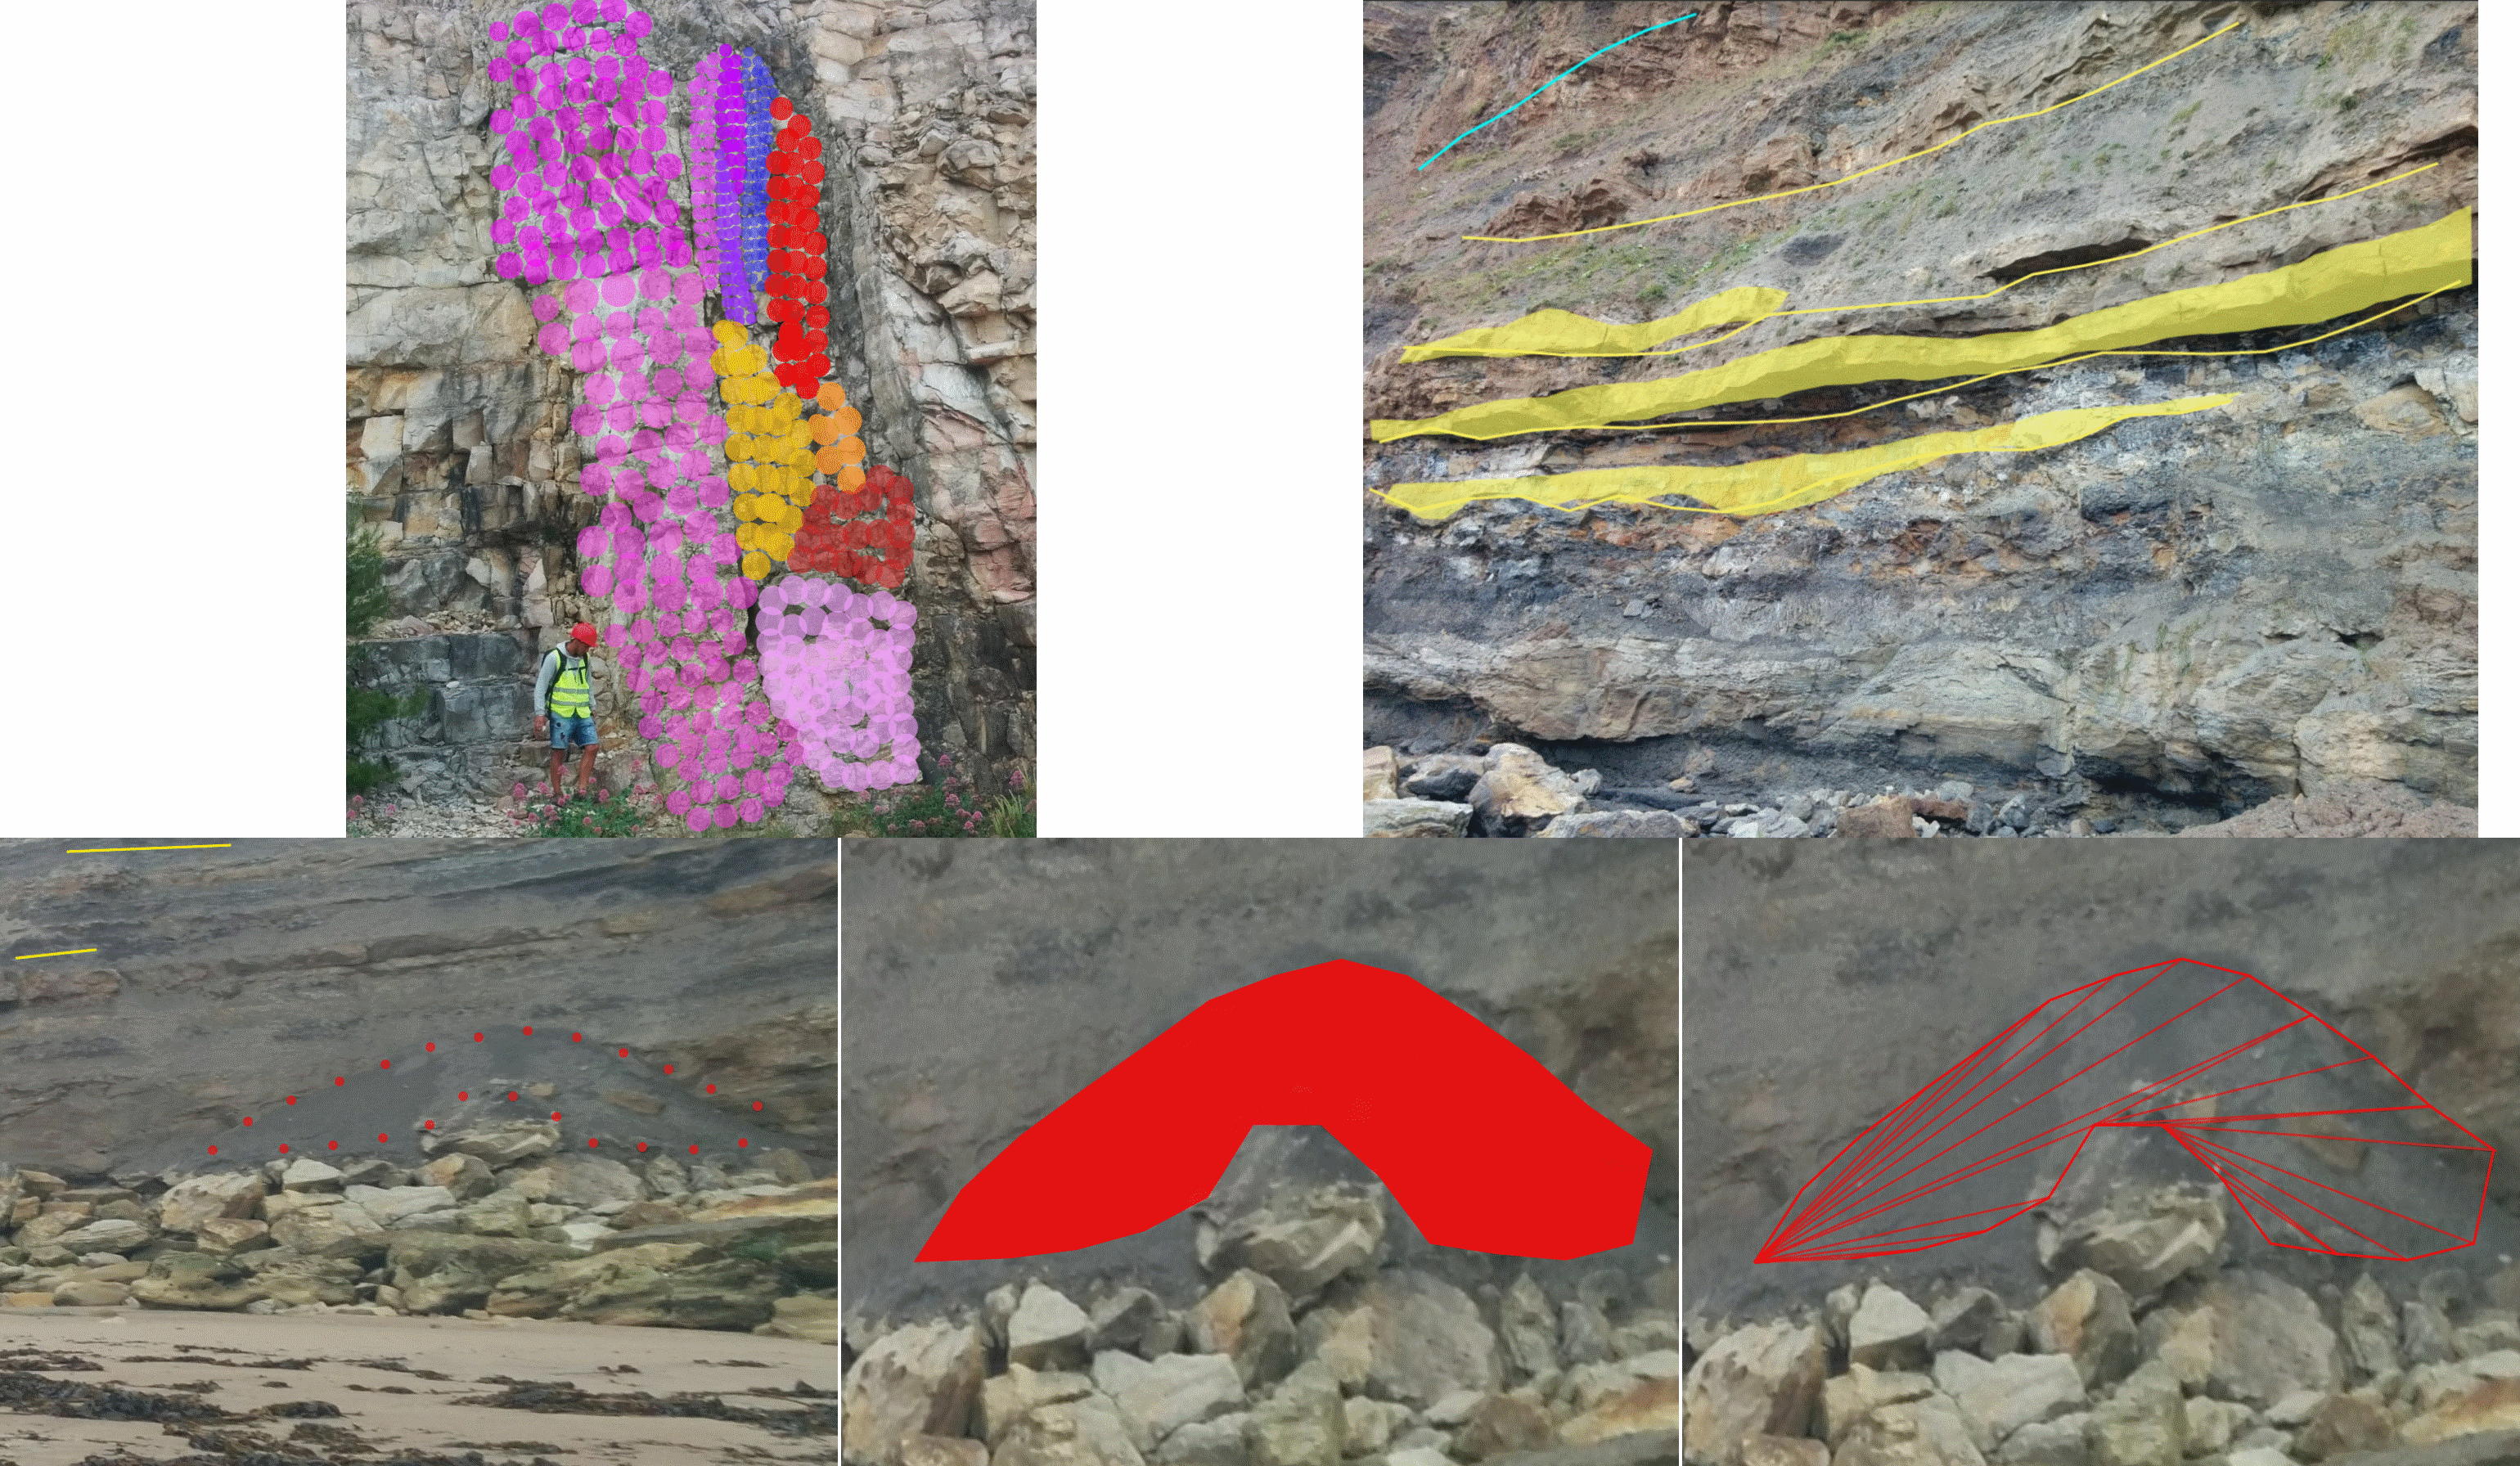
\includegraphics[keepaspectratio, width=0.95\columnwidth, height=6.5cm]{graphics/GRIT_interpretationTools_new}\label{fig:intro:geologicalInterpretationPanel}}
	 	\end{minipage}
	 	\begin{minipage}{\columnwidth}
	 		\centering
			\subfigure[]
			{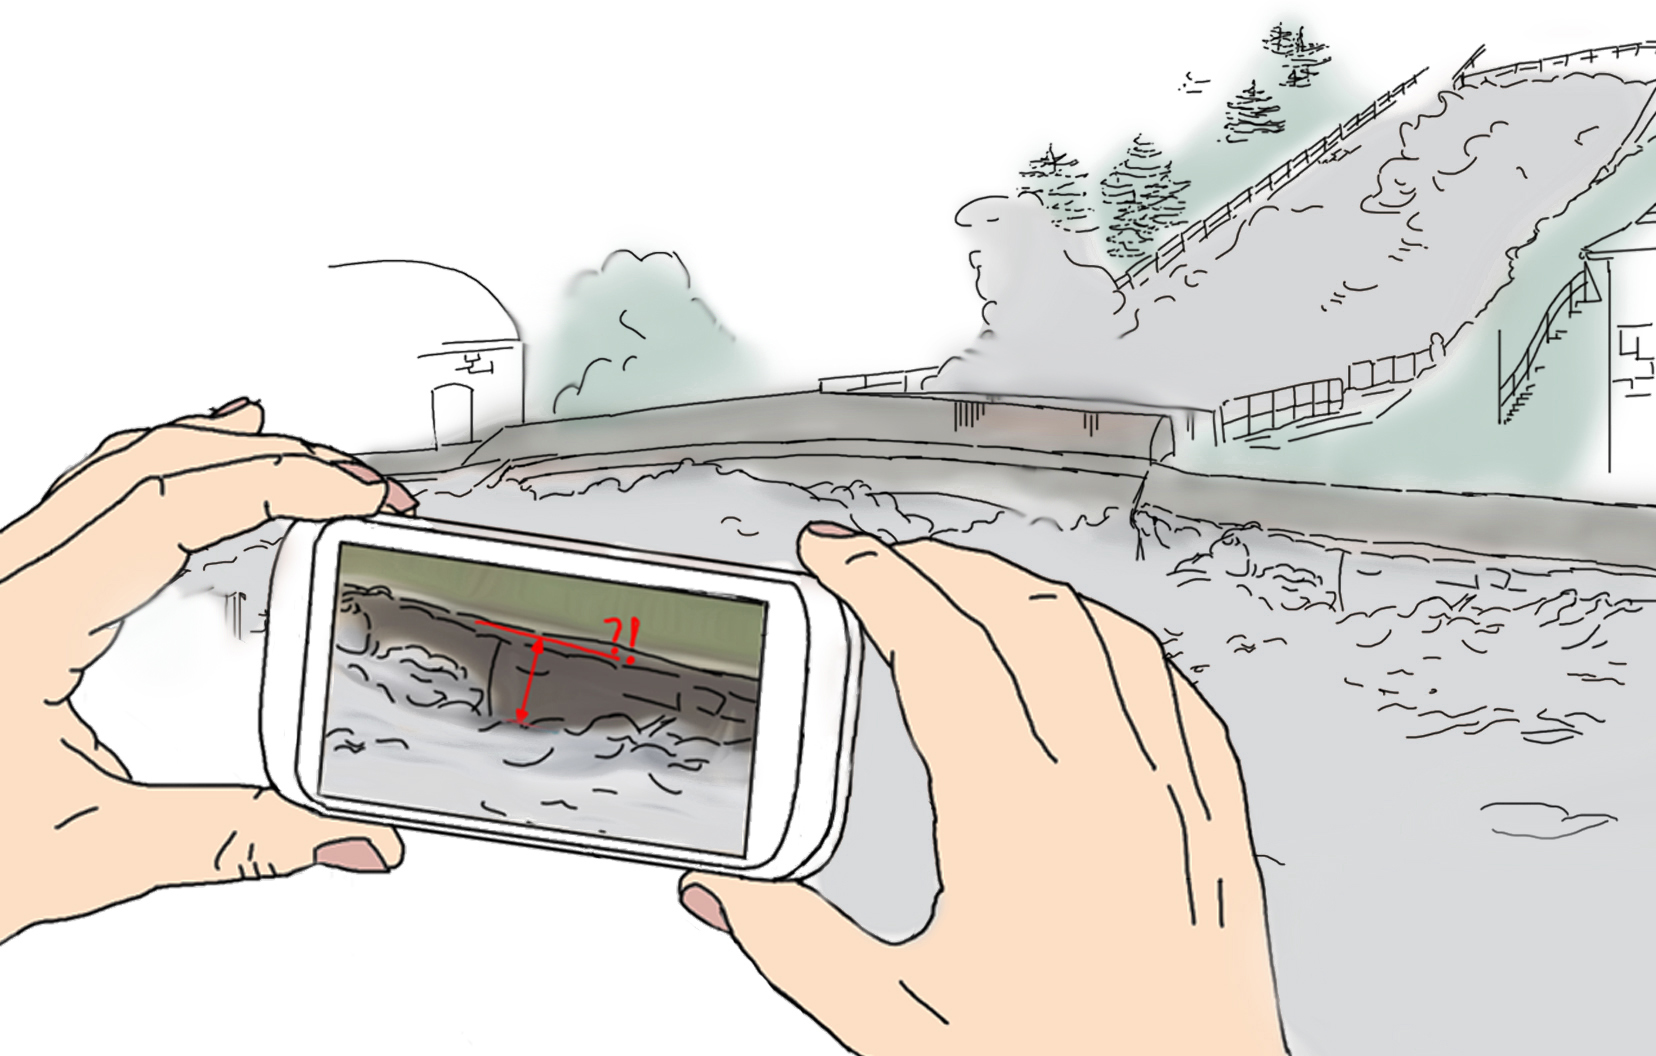
\includegraphics[keepaspectratio, width=0.95\columnwidth, height=6.5cm]{graphics/sketch_water_level_detection}\label{fig:intro:hydrologicalAnnotationPanel}}
	 	\end{minipage}
	\caption{Illustrative examples for geological interpretation (a) and hydrological annotation (b).}
	\label{fig:intro:interpretation}
\end{center}
\end{figure}

\begin{figure}[htbp]
\begin{center}
	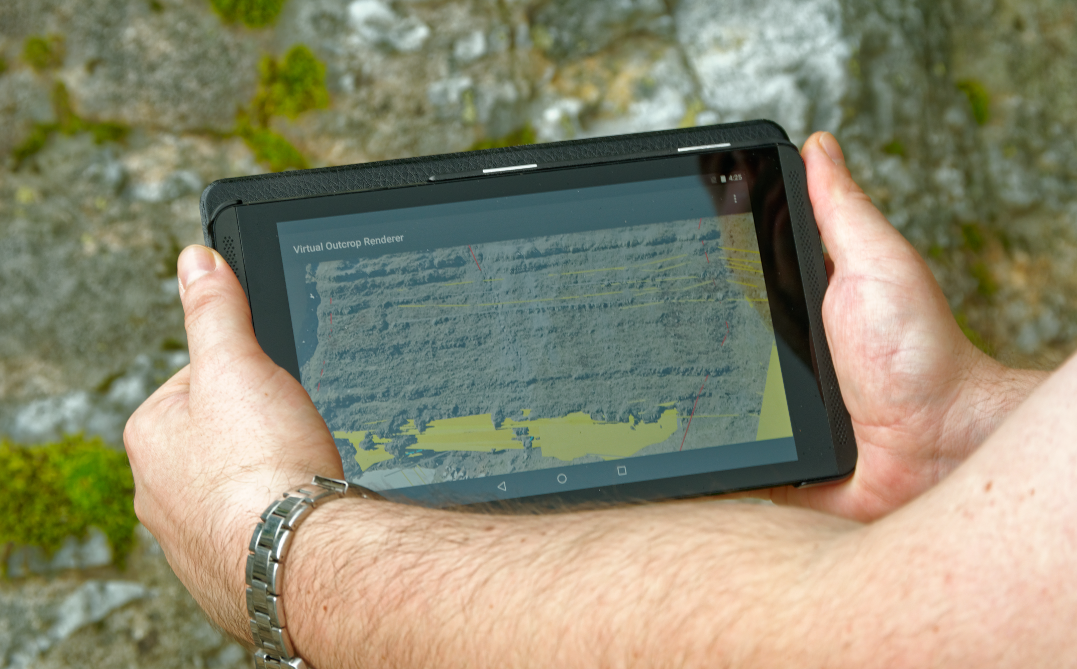
\includegraphics[width=0.95\linewidth]{graphics/GRIT_overhands}
	\caption{Target application of field-based interpretation and annotation on mobile devices.}
	\label{fig:intro:mobileInterpretationInField}
\end{center}
\end{figure}

%\begin{itemize}
%\item Many geosciences domains rely on natural observations and digitised interpretations thereof to steer and constrain numerical models
%\item many semi-automatic interpretation methods have emerged over the years that support digital documentation of observations and interpretations
%\item drawback of existing methods: reliance on computing equipment; the more powerful it is, the more stationary it is
%\item observations within hydrology, geology or glaciology are done outdoor experiments, which prohibit the use of bulky equipment
%\item the advent of mobile computing equipment, such as smartphones and tablets, enable digital interpretations being carried out in the field
%\item smart mobile devices are ubiquitous and easy to equip in field-based research
%\item as seen in technical magazines and the media, the range of available devices increases, which allows to find a device fit-for-purpose to each situation
%\end{itemize}

Next to easily available, pocket-format computing devices, the required three-dimensional base data for modern applications also need to be available and being processed in a ''mobile-ready`` manner. The availability of topographic 3D surface data is steadily increasing due to easy-to-use software and instrumentation for surface generation (e.g. drones, \gls{SfM} \cite{Wu2013} and multi-view geometry \cite{Goesele2007}, satellite \glspl{DEM}). Furthermore, crowdsourced data and \gls{VGI} contribute to the geoscience data inventory, being acquired by citizen scientists. %amateur scientists and domain enthusiasts.

%\begin{itemize}
%\item availability of small form factor devices is only on part contribution to making digital geosciences more ''mobile``
%\item appropriate 3D data needs to be available on these mobile devices to perform interpretations
%\item availability of 3D surface models increases, due to easy-to-use software and instrumentation (e.g. drones, \gls{SfM}, satellite \glspl{DEM})
%\item crowdsourced data and \gls{VGI} constitute to the geoscience data arsenal, being acquired from amateur scientists and novices interested in a particular domain
%\end{itemize}

Domain-specific mobile software is required in order allow for data interaction on the available mobile devices. Specific challenges such as power consumption, multi-manufacturer support, smart sensor utilisation and device intercommunication distinguish mobile software from common desktop software. This leads to a very different electronics design of tablets and smartphones compared to desktop PCs and laptops. In return, this means that existing approaches for digital data processing and interpretation are not transferable as--is to this new computing domain. Even when considering the fast technological development, there are some challenges within mobile device software development that are rooted in the technology itself: user interfaces need to be designed specifically for touch screen interfaces, natural language interfaces and gesture interaction (e.g. ''swipe`` and ''optical lens`` motions). \Gls{GNSS}-based localisation accuracy, as delivered by the integrated-circuit sensor of mobile devices, is inferior to common user expectations and requirements in geoscientific studies. The modalities of sensor data delivery (be it hardware sensor or software emulation), photo capturing and processing, and the computational capabilities of mobile devices differ significantly between each vendors. Short-comings, such as inappropriate data structuring, visual object correlation and registration, increasing data volumes and the unavailability of off-the-shelf program codes, further complicate the technological development. Addressing the demonstrated challenges distinguishes the mobile application development and common desktop software development for geoscience purposes. \textcolor{red}{[...] You agree? Mel: got it! yes, totally agree and very good point!}

%\begin{itemize}
%\item In order to connect data and devices in the field, domain-specific mobile software is required
%\item specific demands and challenges, such as energy efficiency, multi-manufacturer support, smart sensor utilisation and device communication, distinguish mobile software from common desktop software
%\item existing approaches for data interpretation are not transferable as--is to mobile devices
%\item new application cases, which are demonstrated and discussed in this article, and an increasing interest from geoscience- and computer technology industry lead to an increasing interest in this cross-disciplinary domain between mobile computing and geoscientific interpretation
%\item Even considering the fast technological development, some challenges around mobile device development exists that are rooted in the technology itself
%\item user interfaces need to be specifically designed for mobile devices, utilising touch interfaces, natural language interfaces and gestures (e.g. ''swipe´´ motions)
%\item short-comings in geo-localization accuracy, object matching- and registration accuracy, geometric- and photometric data processing, data volumes and the availability of off-the-shelf program codes further complicate mobile device development
%\item technical details such as device variability, power consumption and computing efficiency (i.e. fast calculations with drastically limited computing capabilities) also need to be address during software development
%\item addressing the demonstrated challenges distinguish the complications domain-specific mobile application development pose in comparison to common desktop software
%\end{itemize}

This article demonstrates how the above-listed challenges can be addressed to provide, in the end, the desired added value for field-based research. This demonstration addresses the 3D data annotation and interpretation for two use cases within the domains of surface hydrology and (petroleum) geology. The content covered in the article is a detail-driven extension of earlier published research \cite{Kroehnert2017b}, focussing on extensive measurements to verify the reasoning and statements of previous studies.

%\begin{itemize}
%\item this article demonstrates how the above-listed challenges can be address on two use cases within the domains of hydrology and geology, adding the desired value to digital field-based observation and interpretation
%\item the content covered in the article is an detail-driven extension of earlier published research \cite{Kroehnert2017b}, focussing on extensive measurements to verify previous studies on a more general level
%\end{itemize}

The sections within this article adhere to the following structure: First, the use cases are presented as opening statements to introduce field-related tasks that are to be addressed with mobile device technology. Secondly, different 3D surface data representations are introduced that employed within this technical research. Thirdly, algorithmic baseline concepts that are key for interpreting 3D data on mobile devices are introduced, summarising project-internal development by the authors as well as referencing key literature on the subject. Fourth, the algorithms are mapped to the specific mobile technologies and components. The technologies and major parameters that impact the target use case applications are highlighted. Finally, we showcase and discuss how available mobile systems are used in application scenarios from hydrology and petroleum geology to improve data analysis and integrate outdoor measurements in digital workflows. Then, the article is finalized with some concluding remarks and a discussion for future developments in this research trajectory.

%\begin{itemize}
%\item For the following sections, the article adheres to following structure:
%\item First, use cases are presented as opening statements to introduce task that are exclusively addressed by mobile devices in the digital geosciences
%\item Secondly, the different forms of 3D surface data representations are introduced that are in use within the digital processing presented in this article
%\item Thirdly, algorithmic baseline concepts that are key for interpreting 3D data on mobile devices are introduced, summarising project-internal development by the authors as well as referencing key literature on the subject
%\item Fourth, the algorithms are mapped to the specific mobile technologies and components. The technologies and major parameters that impact the target use case application are highlighted.
%\item Finally, we showcase and discuss how available mobile systems are used in application scenarios from hydrology and petroleum geology to improve data analysis and integrate outdoor measurements in digital workflows
%\item Then, the article is finalized with some concluding remarks and a discussion for future developments in this research trajectory
%\end{itemize}

\section{Target case studies}
\label{sec:case_studies}

The focus in this study is to assess the applicability of mobile devices and the operational metrics impacting their application in scenarios that annotate or interpreted 3D surface data (common capturing surface topography) that are impacted by certain processes, such as surface fluid flow and sedimentary deposition. Other processes to which this scenario extends are erosional processes (e.g. coastal monitoring \cite{Letortu2017, Medjkane2018}), glacialogical processes (e.g. glacial motion and monitoring \cite{Schwalbe2017b}) and landslides.

The case studies feature common challenges and tasks: Given a 3D surface model being observed from a given viewpoint (combining observation position and three-dimensional view direction), features in the topography are to be delineated  in a pre-defined geo-referencing context. The delineation can be approximately horizontal to the average surface, as being the case for water level gauging, diagonal, as the case for tracking the moving front of glaciers relative to the embedding landscape, or embedded as free forms within the topography, such as for landslide boundaries as well as geological element boundaries. The delineations document observations or interpretations relative to the topography.

In a traditional perspective, a key metric for the documentation quality is the metric accuracy of the digitised line delineation relative to the actual real-world position of the observation, e.g. the average distance in real-world metrics. The required metric accuracy can vary between the different application purposes. This can be expressed also in the difference between observation and interpretation: observations target the documentation of an actually visible feature, and thus usually requires higher accuracy than interpretation documentation, as the interpretation itself is a synthesis of direct observation and its interpolation due to domain-specific knowledge.

In relation to mobile technology and mobile-assisted mapping, this traditional metric is difficult to assess. In such application setting, the achievable accuracy depends largely on the accuracy, the georeferencing and the sample resolution of the underlying 3D model that has been formerly acquired. In modern scenarios, there is an increasing demand of making use of existing, freely available topographic models for comparability and cost reduction, which therefore the mobile application has no influence on. An even larger degree of influence is exerted on the other end of the observation -- specifically: the view point. Using mobile devices, the accuracy of the view point directly depends on the accuracy of the delivered sensor information (e.g. magnetic orientation, \gls{GNSS} localisation). Furthermore, as shown below and previously assessed in the literature \cite{Meek2012,Blum2013,Kehl2015c,Novakova2017},  the accuracy range of these sensor information is very broad, it depends on the environment circumstances and even on the assembly of a specific mobile device. Furthermore, the raw signal is processed by dedicated hardware drivers in the operation system by non-transparent and possibly statistical methods and stochastic sampling. Based on these information, it is questionable and problematic to give a fixed measure on the accuracy of such measurements.

Mobile devices, their casual use and their ability to capture new measurements, pictures and digital interpretations and annotations provides a user-driven solution in this case. It appears that letting the domain expert verify the quality of a specific mapping as being ''good enough`` or discard the mapping and redo the measurement- and interpretation process is a viable strategy to achieve the desired quality. The strategy is an option that is prohibited for previous, highly professional mapping products due to their considerable time expense in the creation process.

The specific case studies covered in this article cover surface hydrology and field geology. The former application attempts to document horizontal water level gauge observations for free surface flow hydrology in river catchments with a high degree of mapping accuracy. In order to feasibly achieve this accuracy in the mapping, the presented \textit{Open Water Level} software makes use of temporally correlated image sequences from time lapse series. The latter application maps user-defined free form interpretations on the rock face of an outcrop to delineate geological element boundaries, facies, and supplementary depositional information. Time lapse series acquisition requires multiple camera shots to be captured which draws extra power. Power consumption is a major concern for field geology, therefore reducing the mapping basis to single shots and short-term sensor interpolations. Due to the documentation of interpretations, the hard power requirement and the free form of the delineating without easy constraint formulation, the final line mapping accuracy is necessarily relaxed compared to water level gauging.

\section{Representation basis -- Geometry and Radiometry}
\label{sec:representations}

Various representation forms for 3D terrain data are available. While early digital systems used gridded \glspl{DEM} for their simplicity and compact storage \cite{Trinks2005,McCaffrey2005}, \glspl{DSM} and \glspl{TIN} are dominating most terrain-based systems for application-specific analysis \cite{Buckley2008a,Caumon2013}. A useful example can be seen in \cite{Schwalbe2017b} for glaciology, where the authors use a  triangulated digital surface model to represent a Patagonian glacier front.
%Examples can be seen computing the impact of solar shade on glacial mass loss \cite{Marsh2012}, where the authors use high-quality Delaunay-\glspl{TIN} \cite{Shewchuk1996} as terrain representation. 
For triangular surfaces, it is important to distinguish geometrically valid \glspl{TIN} from polygon soup surfaces (fig. \ref{fig:representations:meshDistinction}). While the latter is often employed in early stages of mesh-based software systems due to its simplicity and ease of implementation, valid \glspl{TIN} are employed in mature stages of the analysis. This is because some automated analysis (e.g. auto-interpretation, volume derivation) require clean surfaces with coherently outward-oriented surface normals.

\begin{figure}[htbp]
\begin{center}
	 	\begin{minipage}{\columnwidth}
	 		\centering
			\subfigure[piecewise-linear complex (PLC)]
			{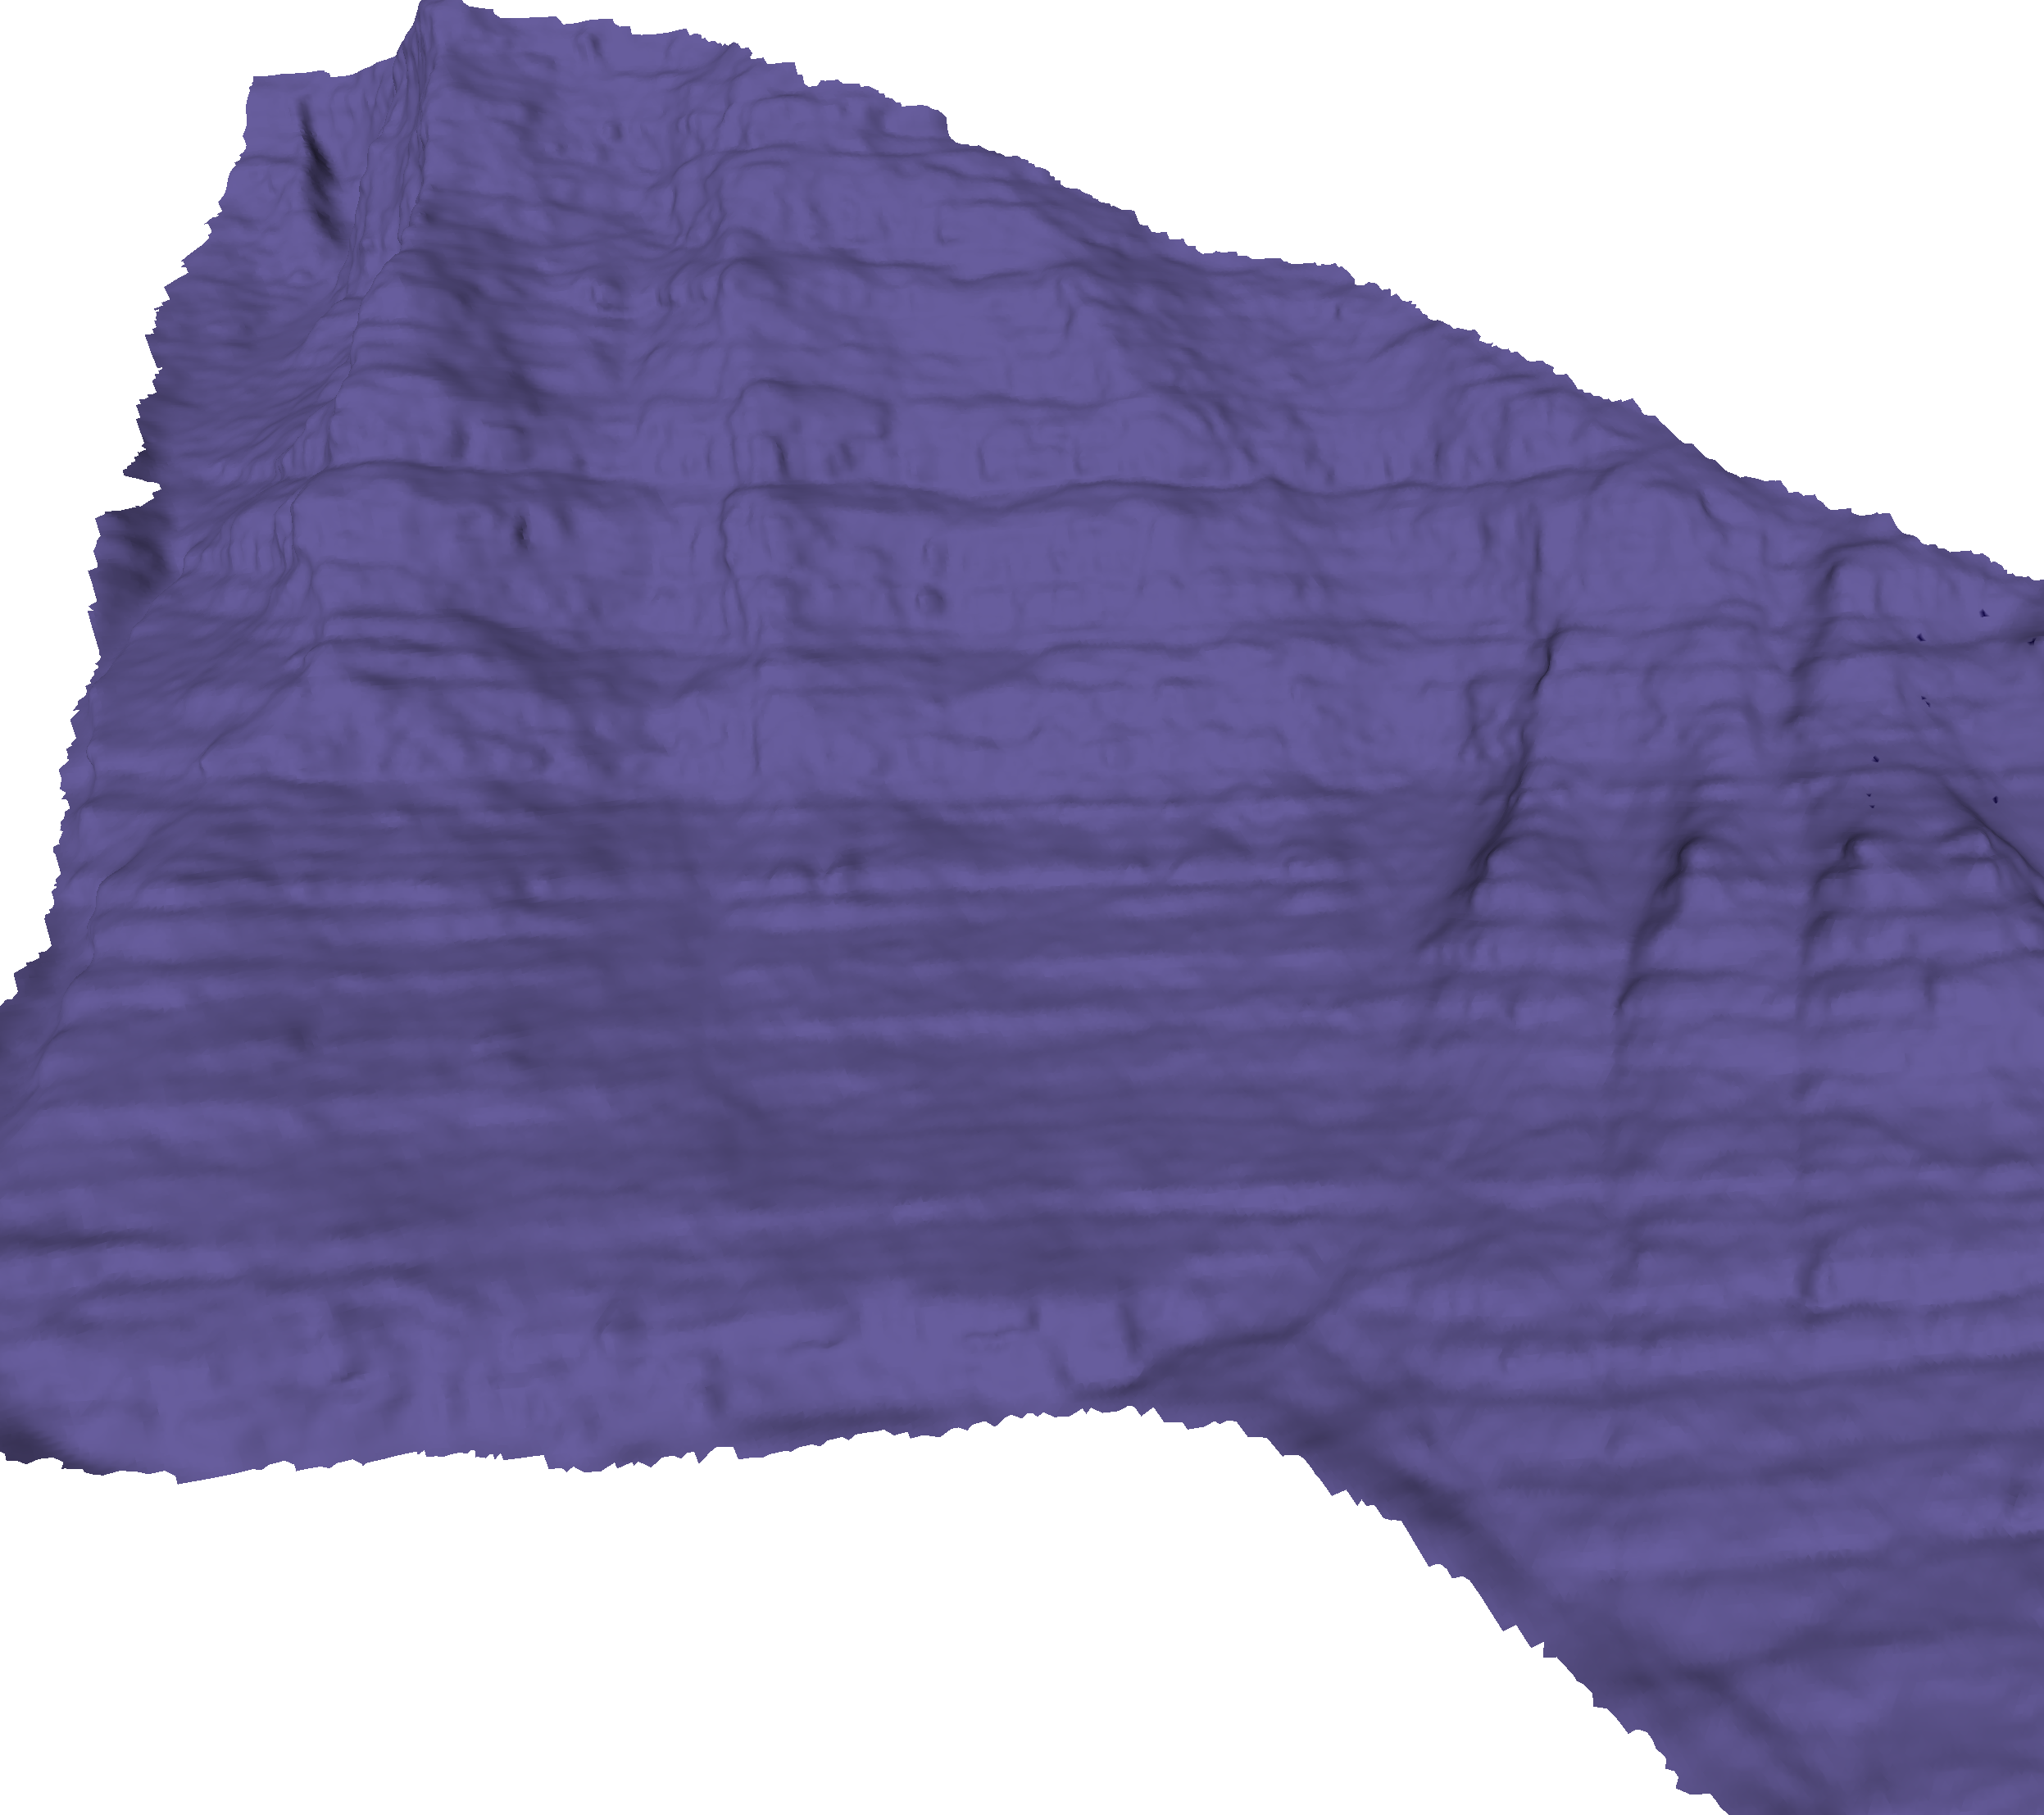
\includegraphics[keepaspectratio, width=0.44\columnwidth]{graphics/MamTor_PLC_MeshLab}\label{fig:representations:PLC}}
			\subfigure[polygonal soup]
			{\includegraphics[keepaspectratio, width=0.44\columnwidth]{graphics/MamTor_TexSurf_composed}\label{fig:representations:polygonSoup}}
	 	\end{minipage}
	\caption{Illustrative distinction between valid \glspl{TIN} (consisting of one exclusive, smooth, closed surface) and polygonal soups. Non-textured model parts are coloured with respect to their actual segment number. Images taken from \cite{Kehl2017_PhDThesis}}
	\label{fig:representations:meshDistinction}
\end{center}
\end{figure}

In geoscience domains such as petroleum geology, texture- and color information are vital for interpretation- and analysis tasks. In these cases, as demonstrated by Buckley et. al \cite{Buckley2008a} and Caumon et. al \cite{Caumon2013}, the \gls{TIN} is supplemented with photographic information that is projected on the surface as textures. The models are referred to as \glspl{DOM} (see fig. \ref{fig:representations:DOM} as reference depiction).% As it is also possible to project textures from outside the visible spectrum as supplementary information on the surface \cite{Kurz2011}, we generalize for the remainder of the article that the model in question consists of its geometric and radiometric information.


%[ASK SIMON FOR USAGE OF IMAGES FROM VOG - use own reconstruction of Whitby cliffs for nice TINs]
\begin{figure}[htbp]
\begin{center}
	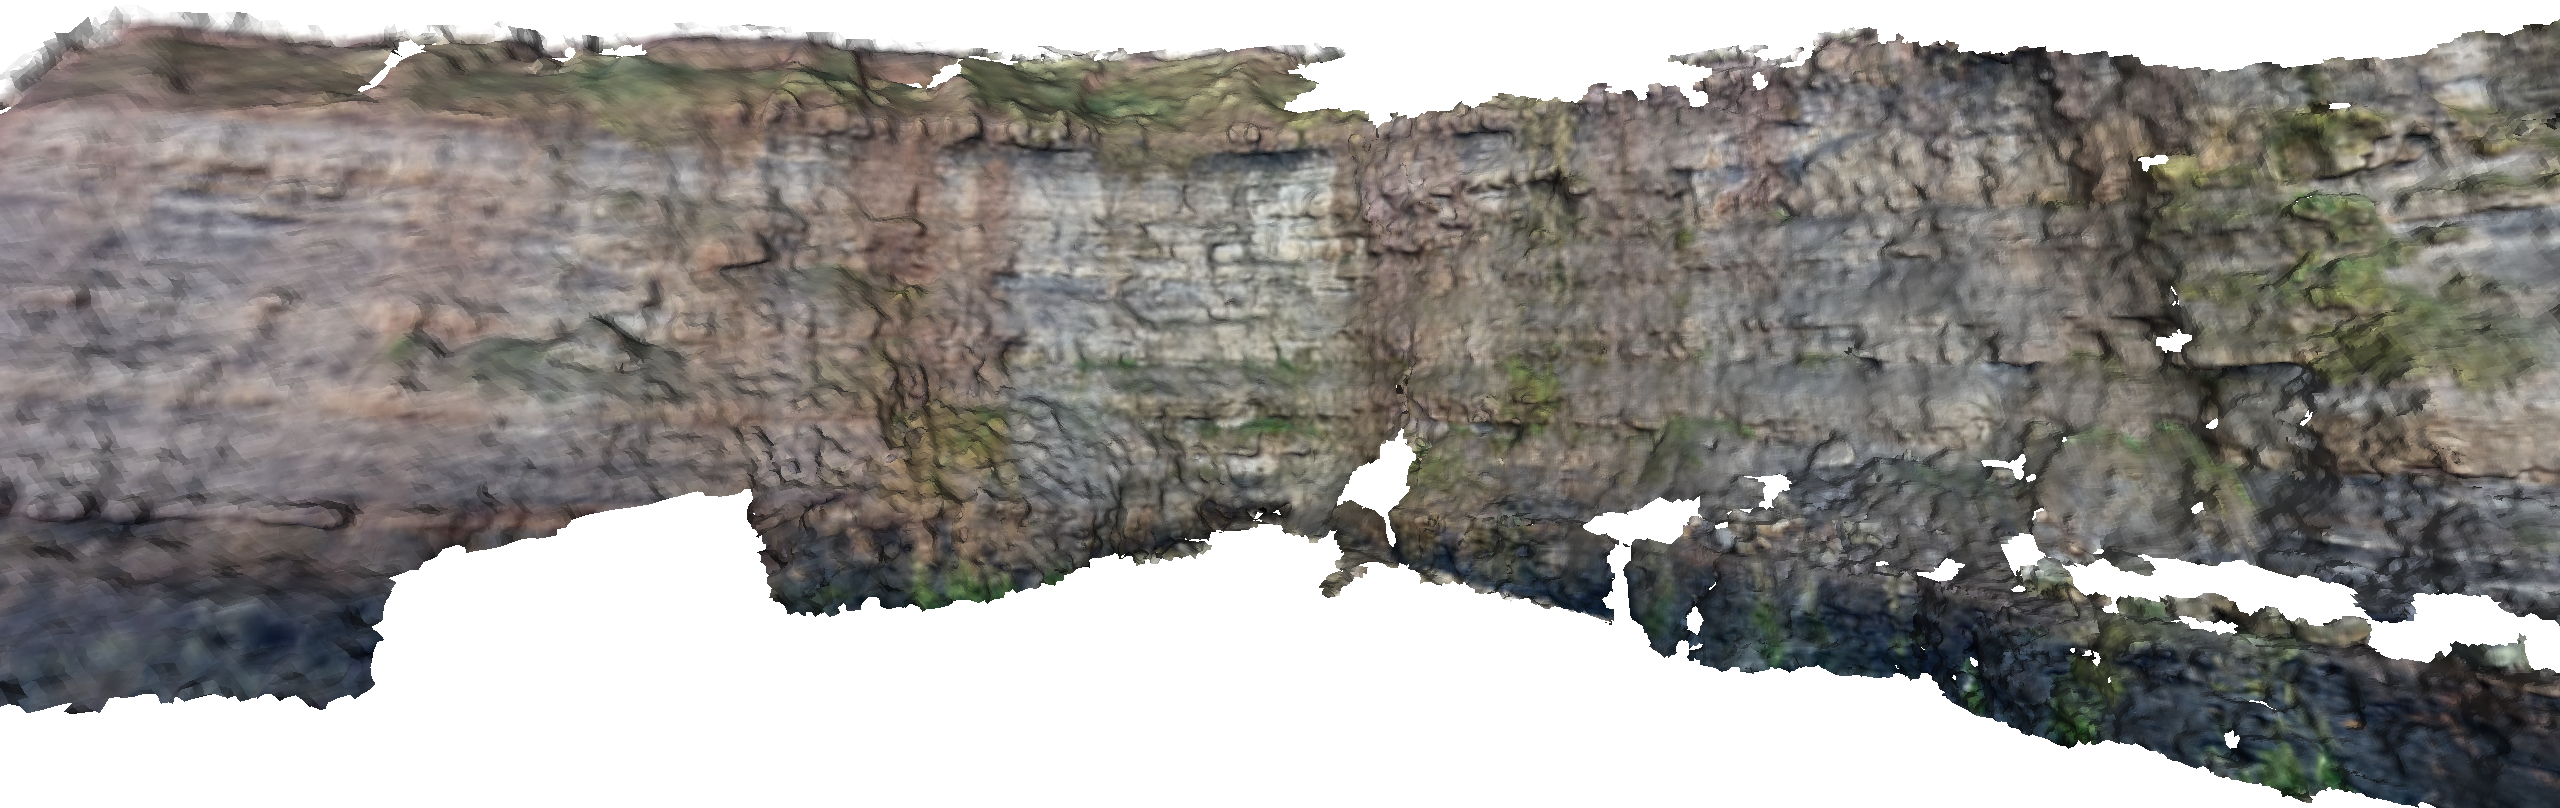
\includegraphics[width=0.95\linewidth]{graphics/DOM00}
	\caption{Example of a \gls{DOM} as textured triangular surface.}
	\label{fig:representations:DOM}
\end{center}
\end{figure}

In contrast, other geoscience domains, such as hydrology and free surface flow management, georeferenced laser scanner point clouds and coloured point data streams provided by terrestrial photogrammetry for small- or \gls{UAV} for large-scale use cases%, both processed by application of \gls{SfM},
 are used. The point set surface data support tasks like coastal monitoring \cite{Letortu2017, Medjkane2018}, soil erosion and rain-induced landslide observation, even monitoring river's topography \cite{Watanabe2016} and even flood protection management \cite{Leskens2015}. Nevertheless, new approaches for low-cost and on-the-fly river monitoring \cite{Kroehnert2017a} arise due to globally increasing flash flood events after heavy rainfalls \cite{Mueller2011} that are further addressed in section \ref{sec:water_level_gauging_intro}.
 
Since \gls{SfM} became state of the art in geosciences, the acquisition of (true-)coloured ''point cloud`` models is not that difficult and commonly employed because of its rapid processing (compared to conventional approaches like \gls{TLS}). Regarding 3D annotation, nearest neighbour analysis provides an opportunity whereby surface triangulation can be avoided.

%%\sout{... colored point data streams are used as models, which are provided by \gls{UAV} and \gls{SfM} Presentation techniques (i.e. rendering) are in these cases adapted versions of \gls{PBR} \cite{Rusinkiewicz2000}. Examples of point-based surface analysis in hydrology can be found in Leskens et. al \cite{Leskens2015}, whereas \gls{VRGS} is an example software for petroleum geology that employs similar techniques (see Rarity et. al \cite{Rarity2014}).} \textbf{HERE MELANIE'S PASSAGE}

The stated base concepts of geometric representation and radiometric texture information are also valid for mobile device software. Because of the limited processing speed of mobile chipsets, the usage of point cloud appears most common within the graphics literature (e.g. Garcia et. al \cite{Garcia2015}). The sparse vertex distribution in point clouds causes problems in the data analysis, which is why \glspl{DEM} have seen a revival in the mobile computing domain. \Glspl{DEM} provide dense, closed geometric models that can be rendered and processed efficiently. Furthermore, with the inferior memory capacity of mobile devices in comparison to laptops and workstations, the possible compression options for point clouds and \glspl{DEM} are advantageous. Base mapping applications such as Google Maps use \glspl{DEM}, derived from \gls{LiDAR} or satellite data \cite{Farr2007}, as their main topographic data representation. Other 3D processing systems on mobile devices within the geosciences, such as ''Outcrop`` and \gls{GRIT}, employ genuine textured triangulated \gls{DSM}.% from \gls{LiDAR}, drone or \gls{SfM} sources.

The chosen form of model representation significantly impacts the algorithms and analytical capabilities employed on the mobile device. Although all algorithms presented in this article work on either form of representation, some of the algorithms favour the treatment of triangulated surfaces (e.g. image-to-geometry registration, guided interpretation), while others clearly favour point-based representations (e.g. rendering).

\section{Algorithms}
\label{sec:algorithms}

This section demonstrates novel- as well as existing algorithms and methods on mobile devices that provide the basis for case-specific field-based annotation, interpretation and analysis shown in section \ref{sec:case_studies}. As mentioned before, the effectiveness of each algorithm depends on the applied model representation.

%\subsection{Structure-from-Motion (SfM) and  Visual Simultaneous Localization and Mapping (Visual SLAM)}
%
%\begin{itemize}
%\item \sout{short description what it does}
%\item \sout{how is it generally employed}
%\item \sout{relation to mobile devices}
%\item \sout{approaches and implementation known on mobile devices}
%\item integration to the above-mentioned use cases
%\end{itemize}

%\gls{SfM} and visual \gls{SLAM} aim at automatically reconstructing a 3D environment from a stream of images \cite{Snavely2006}. The output of these 3D reconstruction methods are colored point sets (i.e. point clouds). The technique is employed in the geosciences to acquire and measure 3D surfaces and terrain either via a manually collected photo set, or by using drones \cite{Dewez}. The large potential for these algorithms on mobile devices being used directly in the field is that no other equipment was needed the generation of the digital 3D data used for analysis. A powerful mobile devices, such as the Project Tango\footnote{•} or NVIDIA Shield\footnote{•}, is capable of 3D terrain data collection in realtime directly in the field.

%Because of the large potential to all branches in the geosciences to deliver on-spot data acquisition, several research groups have conducted research into that topic. \textbf{FILL IN PARTS FROM THE THESIS HERE!}

%A problem with the listed approaches is their lack of maintenance. There is no readily-available software to this date in the mobile app stores that allows real-time SLAM or SfM. Reasons for the disappearance on previous prototypes can vary, but a major problem is the speed of development for mobile devices. As new operation system versions are published on a half-year to yearly basis, it means that software gets deprecated very rapidly. If no industrial partner cares to maintain and market a given research prototype, then that is vanishing from the mobile software market quickly.

\subsection{Image-to-geometry registration}
\label{sec:algorithms:I2G}

%\begin{itemize}
%\item \sout{short description what it does}
%\item \sout{how is it generally employed}
%\item \sout{relation to mobile devices}
%\item \sout{approaches and implementation known on mobile devices}
%\item integration to the above-mentioned use cases
%\end{itemize}

Image-to-geometry algorithms aim at registering 2D images to a given 3D surface, providing a transformation from the 2D image coordinate system to 3D model coordinate system as follows:

\begin{eqnarray}
\label{eq:i2g:projection}
P' &= \begin{pmatrix}
u \\ v \\ w
\end{pmatrix} &= [ R_{3,3} | T_{1,3} ] \cdot P \\
P &= \begin{pmatrix}
x \\ y \\ z
\end{pmatrix} & \\
P' &\in \mathds{R}^2 &= \frac{P'}{w}
\end{eqnarray}

\begin{center}
$R_{3,3}$.. rotation matrix, $T_{1,3}$.. translation vector, $P$.. 3D point in object space, $P'$.. 2D projected point in image space, $(u,v,w)$.. 2D image coordinates, $(x,y,z)$.. 3D world coordinates
\end{center}


Using this coordinate system transformation in combination with a known interior camera orientation, it is possible to project each image on the surface. Specific objects outlined in the image, such as image-based interpretations, can also be mapped on the surface. In the geosciences, these algorithms are employed to create a direct correlation between 3D model and the screen- or image space on which annotations and interpretations are based on \cite{Kehl2016_ISPRS}.

% POSSIBILITY TO CUT HERE IF NEEDED
Amongst the published literature, feature-based registration algorithms are most common. Here, salient points (e.g. SIFT, SURF, Harris corners) or edges within the photograph and rendered image of the target 3D model are used to establish an image-to-image correlation. 

In order to establish a 2D--3D correlation, there are two prevalent approaches available: for triangle mesh models, the 2D feature locations within the rendered image are raycasted using the virtual camera's vanishing point, the imaging plane, and the 3D surface model (see fig. 2 in \cite{Kehl2016_ISPRS}). The intersection between the ray and a triangle within the mesh results in the correlated 3D coordinate of the 2D feature. An alternative approach is needed for point-based models because the raycasting does not apply to point representations (i.e. points cannot be intersected directly due to their zero-extent). The alternative approach often applied (see \cite{Sibbing2013,Sattler2011,Rodriguez2012,Garcia2015}) employs smart rendering techniques that virtually expand the point into an area feature (e.g. blob, disk or sphere), which is subsequently rendered into a depth map. Afterwards, the 3D coordinate of a 2D feature can be inferred directly from the depth map. Though cleverly utilising graphics technology, this approach is limited by an accuracy-to-speed trade-off: low-resolution and low-quantisation depth maps introduce artificial accuracy errors in the registration process, whereas high-resolution depth maps (above $512^2$ pixels) cost considerable performance in the image generation. This last point is particularly important when employing depth map algorithms on mobile devices.

When 2D--3D point pairs are established, the coordinates are normalized and put into a least-squares optimization system, where the target is to determine the exterior camera parameters ($t_x,t_y,t_z,\psi,\varphi,\theta$) from the 2D--3D point-based equation system. Non-linear optimisation systems (e.g. Levenberg-Marquardt) are applied to estimate the desired parameter set \cite{Torr2000}. The whole process can easily be executed on mobile devices \cite{Kehl2016_ISPRS}. One of the prevalent practical challenges when employing feature-based image-to-geometry registration is to achieve a reliable feature correlation, which is often achieved by introducing application-specific constraints (e.g. horizon alignment, straight-edge enforcement or object outlines).
% END OF CUTTING POSSIBILITY


%\begin{itemize}
%\item feature-based registration: detect prominent points or edges in the input 2D images and a rendered representation of the 3D model
%\item different concept for registration: 
%\begin{itemize}
%\item for mesh models, 2D feature locations are raycasted using camera projection and the 3D model in background; 3D feature location determined upon ray-plane intersection
%\item for point-based models, raycasting doesn't directly work as point cannot be intersected; prominent solution is employing a smart rendering technique that expands the point into an area, and generate a depth map; after depth map generation, the 3D coordinate of a 2D feature map can be read directly from the depth map; drawback of the method / offset for speed: accuracy limitation of depth maps; high-resolution depthmaps (above $512^2$) cost a lot of performance
%\end{itemize}
%\item registration then has source- and target 2D-3D point pairs (in a normalized manner) that are put into a least-squares optimization system (give math here)
%\item optimization system usually non-linear, usually employing Levenberg-Marquardt optimization schemes \cite{Kehl2015c}
%\item largest challenges for feature-based registration: (a) reliable feature correlation and (b) optimization stability; useful constraints can employed in both cases -- such as horizon information, building edges, object outlines -- to increase the registration reliability and accuracy
%\item employing constraints is highly application-dependent
%\end{itemize}

Feature-based registration is the most common approach for establishing image-to-geometry correlation on mobile devices due to its implementation simplicity, its rapid execution speed, its option for application-specific constraints and the wealth of available code that can be used. Examples for the application of the technique are ample within the literature, ranging from augmented reality \cite{Gauglitz2014,Sweeney2015} over field geology \cite{Kehl2016_ISPRS,Kehl2017_VGC} to surface hydrology \cite{Kroehnert2017a,Boerner2016}. These mobile apps utilize the open-source library \textit{OpenCV4Android}\footnote{OpenCV4Android 2.4.10 - \url{https://opencv.org/platforms/android/}}, which is also employed in this work\footnote{OpenCV4Android extensions at \url{https://github.com/CKehl/opencv4Android_extension}}. Problems in real-world cases are posed to this technique from imaging variances, resulting in reduced reliability (i.e. failing to determine any camera parameters) and stability (i.e. determining different parameters for the same sets of images) \cite{Kehl2017_PHOR}. A completely alternative technique to feature-based methods is \gls{MI} \cite{Viola1997,Corsini2013}. \Gls{MI} performs a pixel-wise comparison between the photo $I_{2D}$ and the 2D rendering of the 3D scene $I_{3D}'$ and aims at minimizing the image discrepancies (i.e. $argmin \Delta(I_{2D}, I_{3D}')$). The technique uses information theory quantities such as self-information and entropy in order to compare the similarity of both image (see \cite{Bonaventura2017} for further applications of \gls{MI} within the geosciences). In contrast to feature-based techniques, \gls{MI} faces challenges in the optimization process: the optimization of a 7 degree-of-freedom equation system ($t_x,t_y,t_z,\psi,\varphi,\theta,f$, for $f$ being the focal length) is unstable and prone to rest in local function minima. Only few optimisation solvers are known that can solve such equation systems reliably and provide stable results - most notably NEWUOA (i.e. Powell's method\cite{Powell2006}) used by Corsini et al. \cite{Corsini2013}. As these stable solvers are not available in modern- and mobile-device programming languages, the use of \gls{MI} is currently prohibited for mobile platforms.

%\begin{itemize}
%\item feature-based registration techniques most prevalent on mobile devices due to execution speed, implementation ease and so forth
%\item examples of mobile implementation: \cite{Gauglitz2014,Sweeney2015,Kehl2017_PHOR,KroehnertXYZ}; utilize open source library \textit{OpenCV4Android}\footnote{OpenCV4Android - \url{https://opencv.org/platforms/android/}}, also employed in this work\footnote{OpenCV4Android extensions at \url{https://github.com/CKehl/opencv4Android_extension} and \url{}}
%\item drawback of feature-based methods: reliability and instability to imaging variances (discussed later in this article)
%\item a contrasting technique commonly achieving more accurate results: mutual information
%\item idea: pixel-wise comparison between 2D input image and 2D rendering of 3D scene; if both images match (meaning: $argmin \delta(I_{2D}, I_{3D}')$), then registration is completed
%\item mutual information \cite{Viola1997} use notion of self-information and entropy to measure $\delta(I_{2D}, I_{3D}')$
%\item challenge: optimization of 7 degree-of-freedom system over such overdetermined system (i.e. each image pixel results in 2 equations for the optimization scheme) unstable and prone to local minima
%\item only optimization known to provide stable results is NEWUOA (i.e. Powell's method) \cite{Corsini2013}; 
%\item has recently been employed in an earth science case for \gls{LiDAR} registration \cite{Guislain2016}
%\item not available for mobile devices until now
%\end{itemize}

While the task of image-to-geometry registration can be offloaded to remote computers in the network, it is advantageous to perform the registration on the mobile device itself. This is because, in the overall target of model interpretation, the interaction and actual interpretation (as explained in section \ref{sec:algorithms:interpretation}) is more intuitive for the user when being performed on photos and images. If the registration of the images is done on the mobile device, it allows for direct feedback and ad-hoc visual quality checks of the interpretations on the underlying 3D surface model (see fig. 7 in \cite{Kehl2017_VGC}). Furthermore, as shown by measurements in section \ref{sec:technology:power}, it can be argued that 2D interpretation more energy efficient than direct 3D interpretations. Lastly, in settings where network access and offline processing is prohibited, an on-device registration procedure is without alternatives.

%\begin{itemize}
%\item in terms of usability on mobile devices (why should we want to have that on mobile devices), projection of image-based information is vital on mobile devices
%\item because of interaction difficulty, image-based interpretations on 3D surface data is preferable
%\item it is potentially advantageous, in terms of power consumption, to implement data interaction in 2D rather than 3D; a hypothesis proven by experiment in this article
%\item as it directly relates to the interactive component of the geoscience app, it has to be executed in real-time on the device instead of an offline process
%\end{itemize}

%\subsection{Data presentation and rendering}

%\begin{itemize}
%\item \sout{short description what it does}
%\item \sout{how is it generally employed}
%\item \sout{relation to mobile devices}
%\item \sout{approaches and implementation known on mobile devices}
%\item integration to the above-mentioned use cases
%\end{itemize}

%\begin{itemize}
%\item rendering the 3D model in this context refers to generation of image generation of 3D model by projective rasterization of model data to 2D imaging plane of a virtual camera
%\item rendering is performed to view the 3D model on the mobile device
%\item also employed to generate a reference image used in the image-to-geometry registration and the annotation and interpretation of the data
%\item major concepts: mesh-based rendering and \gls{PBR}
%\item technical details on how this is done covered in the technology section \ref{}
%\end{itemize}

%Rendering a surface model in this context refers to the image generation of the 3D data by projective rasterization to the 2D image plane of a virtual camera. This process is performed on mobile devices for the purpose of model presentation as well as for the generation of a synthetic reference image for image-to-geometry registration. Furthermore, it can be used to synthesize an image from available 3D data for interpretation and annotation in 2D. A common distinction relative to the geometry representation is done between mesh-based rendering and \gls{PBR}. The presented algorithms are also closely linked to the details of the technological implementation of 3D graphics on mobile devices via the \gls{GLES}, referred in more detail in section \ref{}.

\subsection{Mesh-based rendering}
\label{sec:algorithms:mesh_rendering}

Rendering a surface model in this context refers to the image generation of the 3D data by projective rasterization to the 2D image plane of a virtual camera. This process is performed on mobile devices for the purpose of model presentation as well as for the generation of a synthetic reference image for image-to-geometry registration. Furthermore, it can be used to synthesize an image from available 3D data for interpretation and annotation in 2D.

Algorithms for rendering textured triangulated surfaces are well-known amongst technology-affine personnel. In the common rendering pipeline, the textured mesh is transferred as a set of (attributed) vertices and primitive sets (e.g. triangles, polygons) to the \gls{GPU}. The virtual camera is set up using the pre-defined view projection matrix while the graphics primitives are repositioned using the model-related transformation matrix. The rasterizer projects the available 3D information into the camera plane and performs hidden-surface removal. The result is a discrete-space pixel representation. Modern programmable shaders allow in-time vertex decompression (see \cite{Ponchio2016}) as well as texture decompression (see section \ref{sec:technology:graphics}). Available textures are mapped as images on the surface using the texture coordinate vertex attributes. The mesh-based rendering algorithms employed on desktop computers are analogous to mobile devices, whereas the technological details are posing the actual challenges.

%\begin{itemize}
%\item well-known concept
%\item mesh is transferred as vertex set and primitive set (i.e. triangles or polygons, depending on employing \gls{TIN} or polygonal soup geometry) to graphics processor
%\item virtual camera is set up as projective view matrix
%\item primitives are positions in 3D scene via model transformation matrix
%\item rasterizer projects information to camera plane and transforms continuous data into discrete pixel-based representation
%\item in-time decompression can be optionally employed (see \cite{Ponchio2016})
%\item texturing is employed to map image information on the surface; correlation between surface patches and texture images established explicitly beforehand or implicitly defined by geographic coordinate systems (e.g. WGS84 or UTM) for georeferenced surface
%\end{itemize}

\subsection{A novel approach to mobile point-based rendering}
\label{sec:algorithms:pbr}
In comparison to mesh-based rendering, simple point projection seems to be a nice alternative saving computational resources and efforts for post-processing concerning outlier removal due to falsely surface reconstruction (e.g. blobs due to critic point normals) \textcolor{blue}{Chris: what do you refer to as ''critic point normals`` ?}. Thus, we simply project object points onto an image plane using perspetive projection, assuming a distortion-free ideal camera with centred principle point. Thus, the camera matrix $\bf K$ equals identity matrix $\bf I$ and can be neglected in the following equations (based on Szeliski(2010) \textcolor{blue}{please insert proper reference here to avoid confusion}). 

First, applying a six-parameter transformation transfers three-dimensional object points from world reference frame $\vec{X}_W$ into a 3D camera system $\vec{X}_c $ using
\begin{equation}
\vec{X}_c = {\bf R} \left( \vec{X}_W - \vec{X}_0 \right) 
\label{eq:projection_simple}
\end{equation} 

where $\bf R$ is a $3x3$ orthonormal rotation matrix and $\vec{X}_0 $ the translation vector to camera's projection center. For simplicity, the usage of the planar Cartesian UTM system with $x$ pointing to the east and $y$ pointing to the north with respect to the prevalent zone number. For $z$ component, the height over the Earth Gravitational Model 1996 (EGM96) is advisable to use. 

Counting for homogeneous coordinates, we can describe the relation between camera $\vec{X}_c$ and image coordinates $\tilde{x}$ involving their depth components. 
\begin{equation}
\begin{pmatrix}
\tilde{u} \\
\tilde{v} \\
c_c
\end{pmatrix} =
\begin{pmatrix}
x_c \\
y_c \\
z_c
\end{pmatrix}
\end{equation}

For camera's imaging plane, we introduce the constant $c_c$ that defines the distance between camera's sensor and projection center in $[mm]$, which equals focal length $f$. To separate camera sensor system and image system, we use the term $c_c$ when talking about sensor $[mm]$, and $f$ for digital image coordinates $[px]$. For conversion, $c_c$ must be divided by the sensor's pixel pitch. \textcolor{blue}{Chris: The normalization of the projected points to homogeneous coordinates is key in the further processing. This is analogous to the image-to-geometry project in eq. \ref{eq:i2g:projection}, where the projection variable $w$ is replaced with the camera constant $c_c$.}

\textcolor{blue}{Chris:
\sout{For 3D to 2D projection, homogeneous coordinates must be divided by their depth components resulting in inhomogeneous coordinates. [remove following equations,as we have them already.]}
}

\begin{equation}
\vec{X}_{Cam} =
\begin{pmatrix}
\frac{\tilde{u}}{c_c} \\
\frac{\tilde{v}}{c_c} \\
1
\end{pmatrix} = \begin{pmatrix}
\frac{x_c}{z_c} \\
\frac{y_c}{z_c} \\
1
\end{pmatrix}
\end{equation}

\textcolor{blue}{
\sout{Thus, two-dimensional coordinates can be described with}
}
\begin{equation}
\begin{pmatrix}
\tilde{u}\\
\tilde{v}\\
\end{pmatrix}
= \begin{pmatrix}
\frac{x_c}{z_c} \cdot c_c \\
\frac{y_c}{z_c}\cdot c_c
\end{pmatrix}
\label{eq:ut_vt}
\end{equation}

For a final transformation of 2D sensor coordinates into image pixels, we need to shift the image coordinate system to the origin to left upper corner and scale the coordinates from global units in meters per pixel using $p_s$. Thus, we derive image coordinates $(u,v)$ for an ideal camera using

\begin{equation}
\begin{pmatrix}
u\\
v\\
\end{pmatrix}
= \frac{1}{p_s}
\begin{pmatrix}
\frac{x_c}{z_c} \cdot c_c  - {u}_0 \\
\frac{y_c}{z_c}\cdot c_c  - {v}_0 
\end{pmatrix}
\label{eq:final_ps}
\end{equation}

%\textcolor{blue}{Chris: end of current check-read - looks good so far.}

\subsubsection{Calculation of 3D bounding box of interest and image plane}
\textcolor{blue}{\sout{Referring to the described use case of situation-based water level determination using a smartphone-camera based gauge (\ref{sec:water_level_gauging_intro})} In the mobile rendering scenario}, we need to define a region of interest regarding 3D point projection \textcolor{blue}{\sout{to render only}to cull the render content of the virtual camera to the} user's field of view (figure \ref{fig:4_3_bounding_box}). The view frustum's bounding box corner points are calculated using the position and orientation from fused smartphone sensors. Thereby it must be noted, that the heading is used for viewing direction only, tilt and roll are excluded. Because of uncertainties regarding exterior information (section \ref{sec:technology:sensors}), the bounding box must be expanded to cover more object space than described by sensors as well as the camera's field of view. Because of possible noise due to positioning, constants $r$ and $dh$ describe the domain of projection center's uncertainties parallel to image plane. For errors in depth, we define the correction $c = \frac{r}{tan(H)}$ for shifting the projection center along camera axis. 

\begin{figure}[h]
\centering
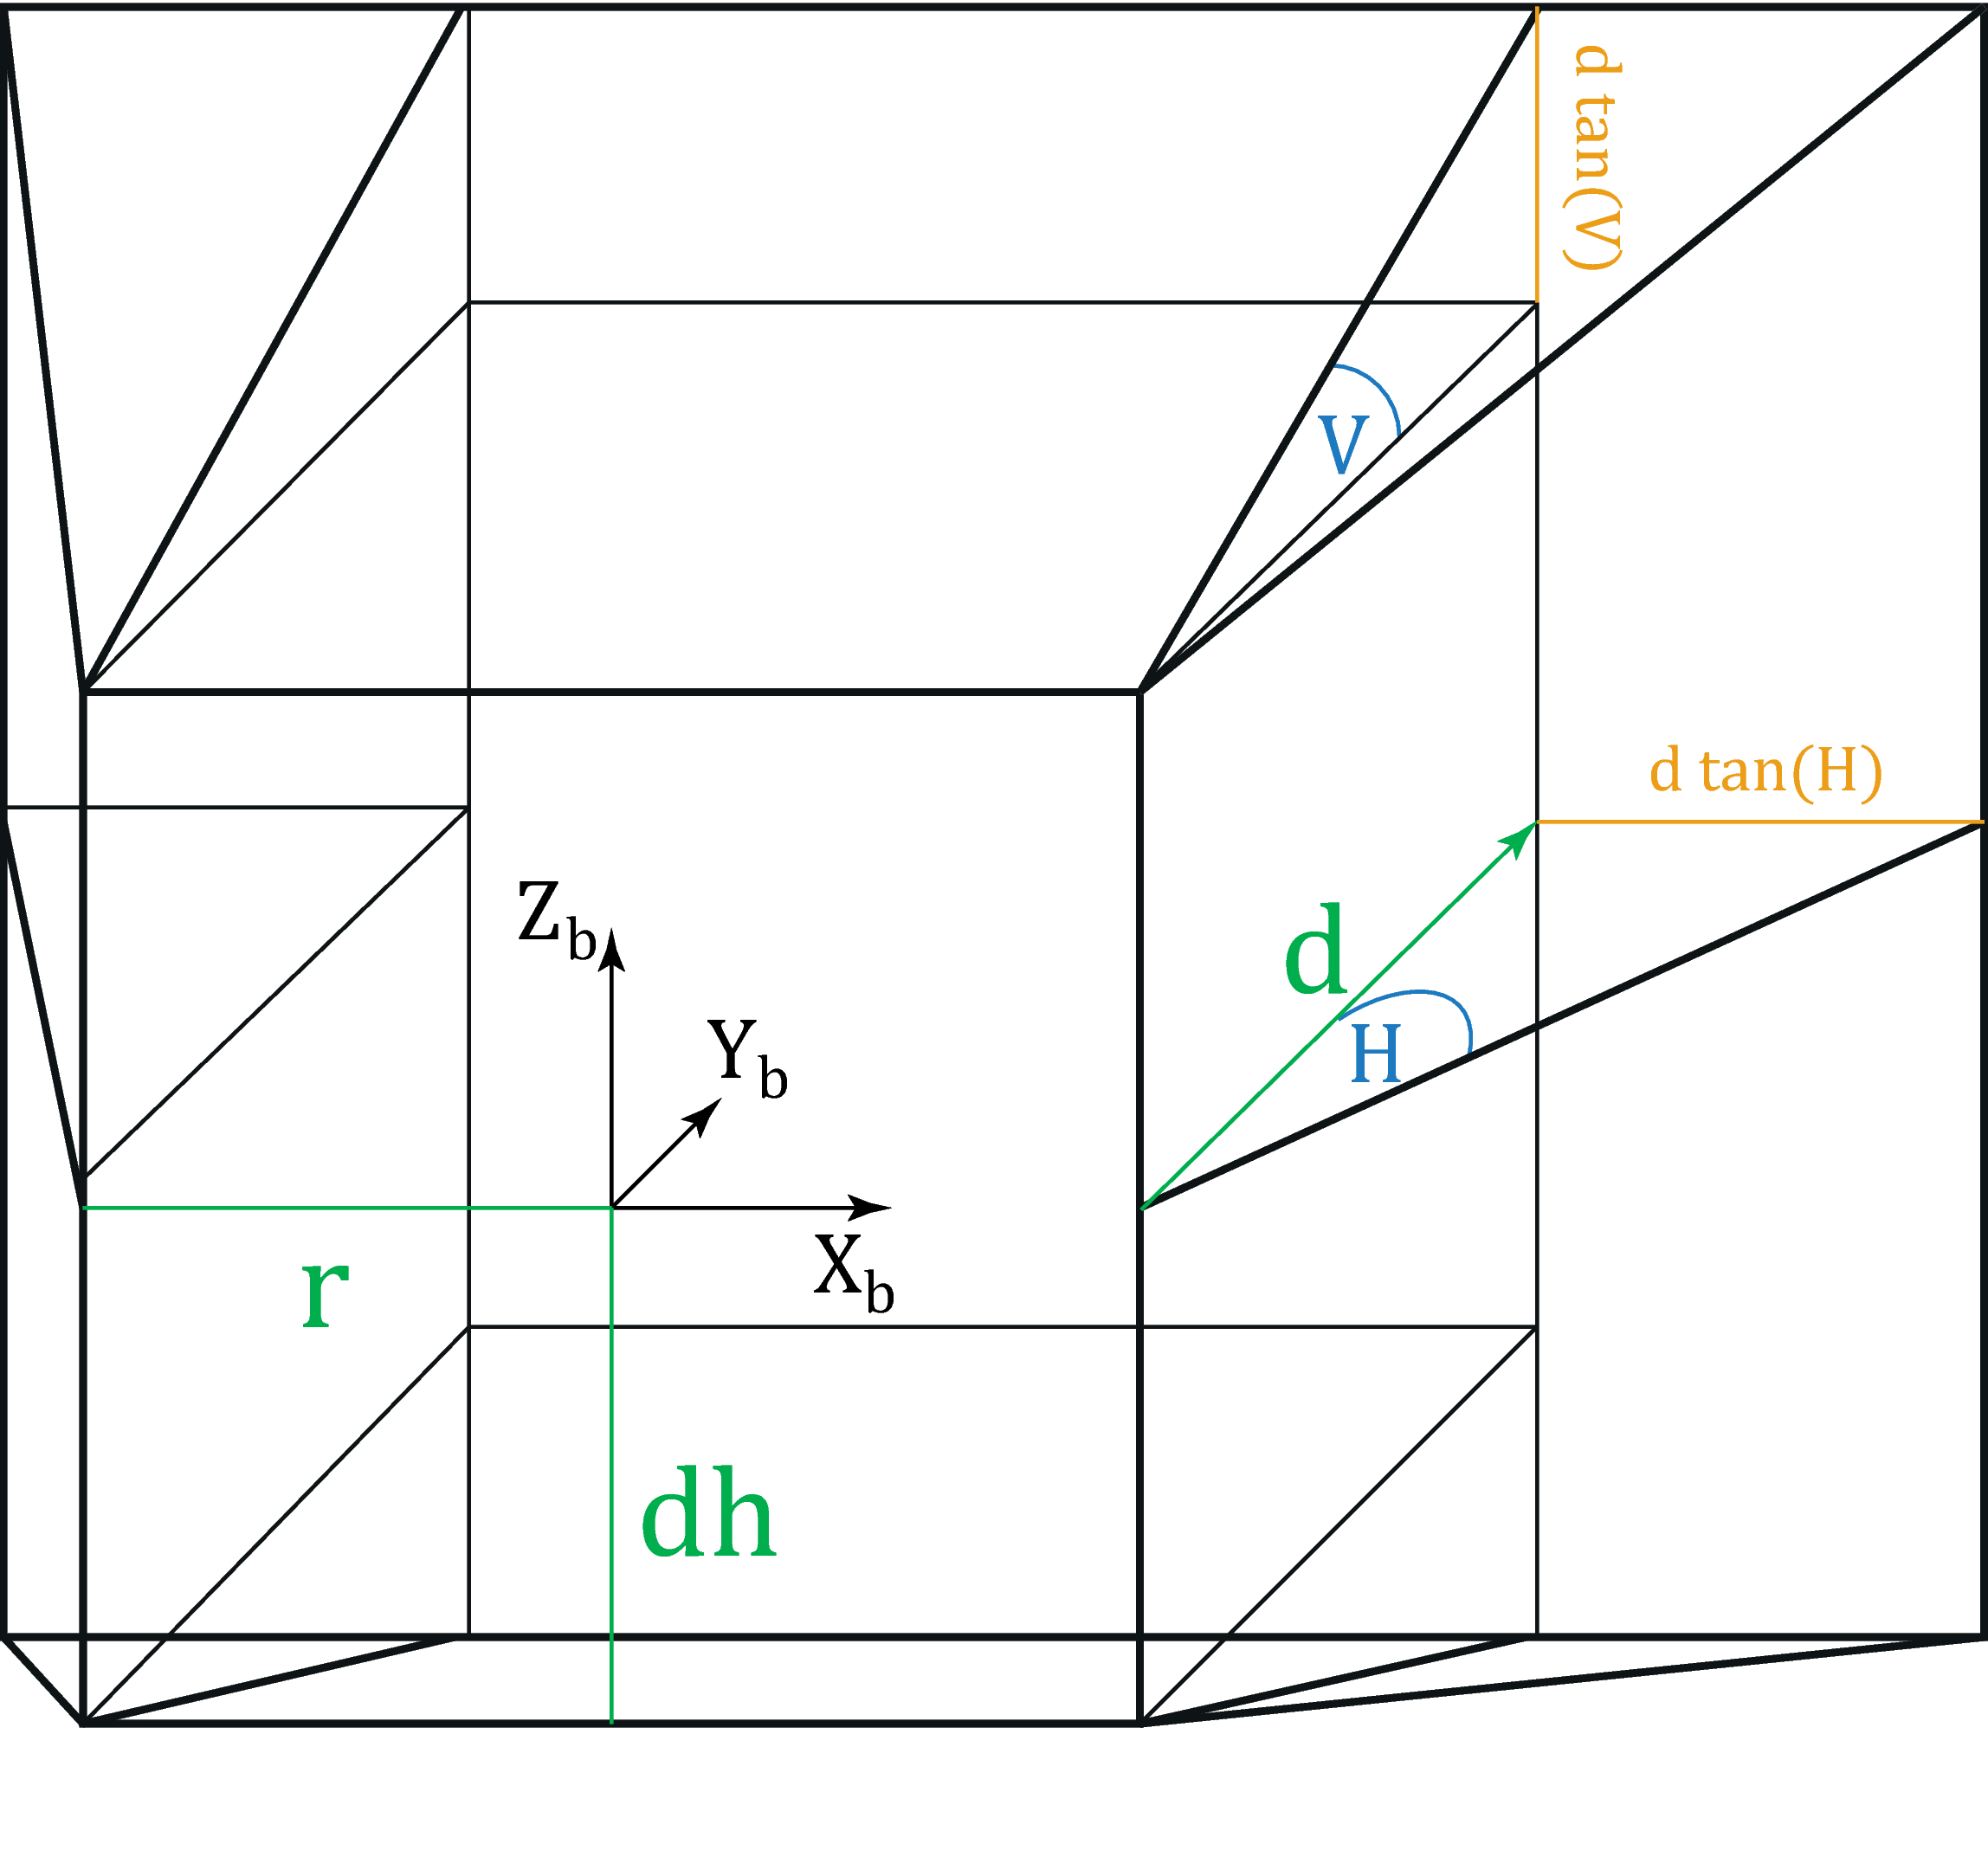
\includegraphics[width=8cm]{graphics/4_3_Bounding_Box}
\caption{Bounding box definition.}
\label{fig:4_3_bounding_box}
\end{figure}

The box is widened by the horizontal $H$ and vertical $V$ opening angles with a fixed depth $d$. In order to generate reference data for image-to-geometry \sout{intersection}registration to annotate 3D data by mobile imagery, the lateral accuracy given by the mobile positioning system as well as the prevalent camera characteristics solve for the mentioned parameters. For camera based gauging, we set $d = 200 [m]$. \sout{Regarding 3D point projection, each potential point will be checked laying in the box. Therefore, additional tiling of the 3D data set is advisable.}Additional tiling of the 3D base data is advisable for a rapid geometry-in-frustum containment check.
Using the defined frustum of a pyramid as region of interest with a local reference system, the image plane for 3D point rendering can be defined by perspective projection of the remote $xz$ plane (\ref{fig:4_3_bounding_box}) with 

\begin{equation}
\vec{X}_b = \begin{pmatrix}
-r - d \tan H \\
d \\
dh + d \tan V
\end{pmatrix}
\notag
\end{equation} 

for bounding box' background plane upper left and 

\begin{equation}
\vec{X}_b =\begin{pmatrix}
r + d \tan H\\
d\\
-dh - d \tan V
\end{pmatrix}
\notag
\end{equation} 

lower right corner. Its height equals the height component in world reference frame $z_w$. Because of pyramid frustum, we have to eliminate outer points between the near- and far clipping plane. \textcolor{red}{workflow for outer point removal necessary?}\textcolor{red}{probably not, unless its deviated from common normal-to-point angular evaluations of the bounding planes or an in-box check per point.}

\subsubsection{Pyramid approach for depth filtering}
Because of a limited range of pixels with defined size inside a image plane it seems to be obvious that in most cases more than one 3D object points corresponds to the same image pixel. Due to inhomogeneous coordinates it is not possible to figure out afterwards which points are in foreground compared to the camera distances and which ones are behind and thus not visible. This problem can easily be solved during point cloud projection described above by a simple camera-to-object distance check. However, one problem still remains in case of e.g. glass fronts with lacking information (in \gls{TLS} due to deflected lidar or \gls{SfM} when having homogeneous surfaces) or small archs (see figure \ref{fig:4_3_dist_images}) Then, points might be visible pointing away from camera projection center. On the one hand, point normals may solve the problem but due to the data acquisition technique and the model's complexity, they are more or less easy to derive \cite{Sattler2011}.

Remedying image pyramids are a nice alternative approach used in this case. Therefore, multiple synthetic images are generated with step-by-step adjustment of $p_s$ (see eq. \ref{eq:final_ps}), commonly by doubling which resulting in halve numbers of image rows and columns per layer. Then, the algorithm verifies if two pixels corresponds in two subsequent layers, preserving edges (figure \ref{fig:4_3_point_filtering},\ref{fig:4_3_dist_images}). \textcolor{blue}{Chris: this sounds a LOT like scale-space image pyramids ... correct ?}

\begin{figure}[h]
\centering
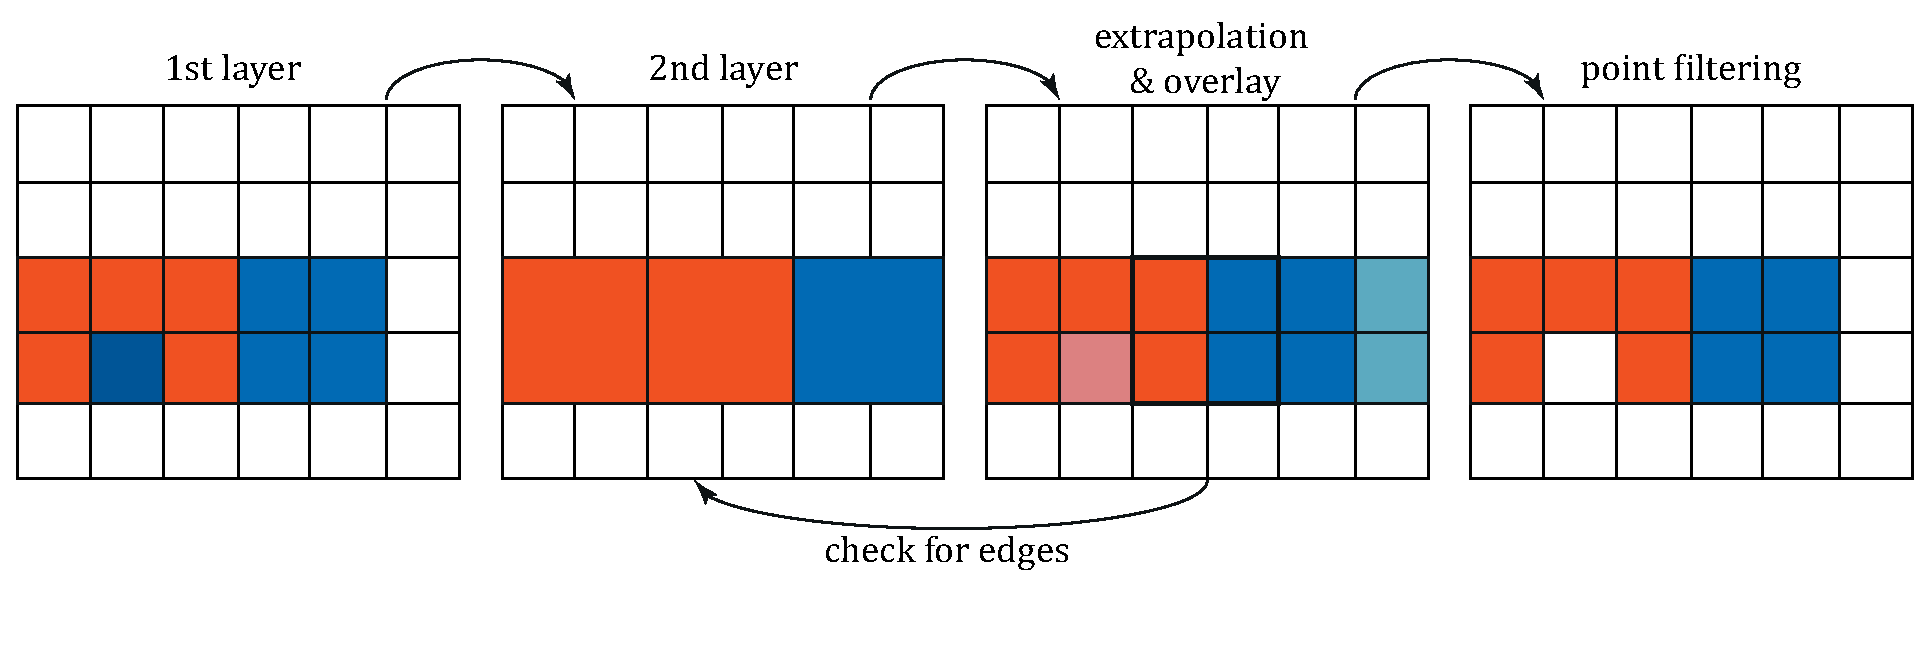
\includegraphics[width=12cm]{graphics/4_3_point_filtering}
\caption{Visualisation of hierarchical depth filtering to handle point occlusions.}
\label{fig:4_3_point_filtering}
\end{figure}
\begin{figure}[h]
\centering
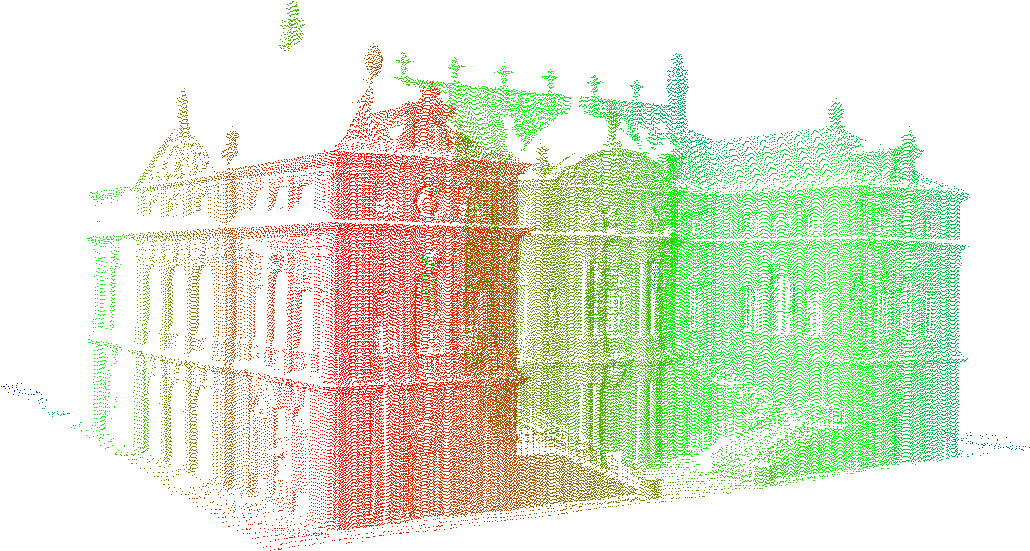
\includegraphics[width=5cm]{graphics/4_3_dist_image_orig}%
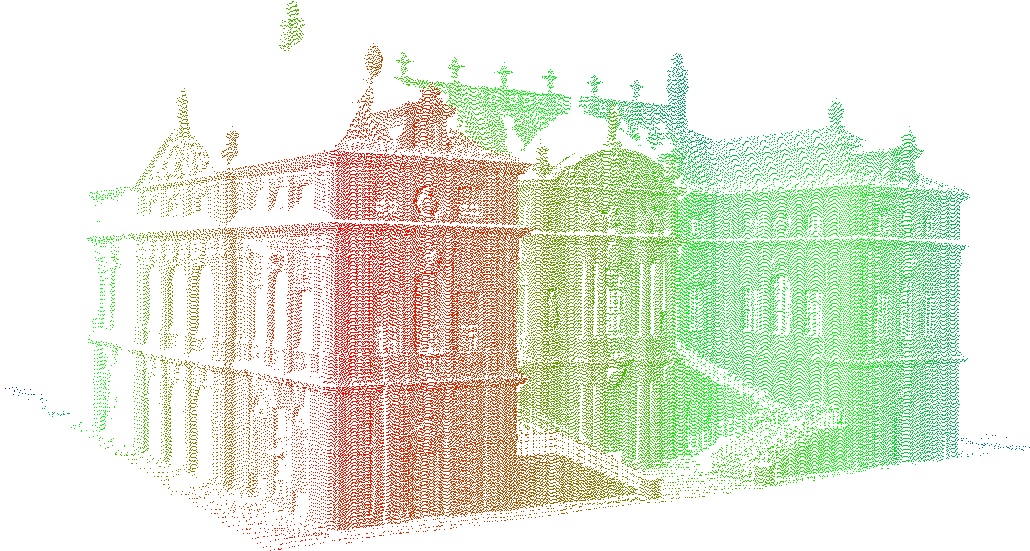
\includegraphics[width=5cm]{graphics/4_3_dist_image_filt}%
\caption{Left, actually obscured visible 3D points close to archs and windows. Right, edge preserving result after filtering.}
\label{fig:4_3_dist_images}
\end{figure}


\subsubsection{Filling gaps due to missing points}
Because of pixel size and image plane definition with a specific resolution (that depending on smartphone full-scale camera's resolution for image registration purposes) there will still be gaps between projected points (see figure \ref{fig:4_3_dist_images}, right). To fill these gaps, we recommend to use a simple nearest neighbour approach using binary search \cite{Bentley1975} in 3D domain to fill these gaps applying weights to average 3D points color attributes depending on their euclidean distances. For this, thresholds for maximum distances between 3D points must be applied to avoid unreasonable gap-filling. Exemplary for use case in section \ref{sec:water_level_gauging_intro}, a before--after comparison of the gap filling is visualised in figure \ref{fig:4_3_fill_images_before_after}.

\begin{figure}[h]
\centering
\includegraphics[width=12cm]{graphics/4_3_fill_images_before_after}
\caption{Fill image gaps using nearest neighbour binary search in 3D domain.}
\label{fig:4_3_fill_images_before_after}
\end{figure}


\subsection{Interpretation and annotation}
\label{sec:algorithms:interpretation}
%\begin{itemize}
%\item \sout{short description what it does}
%\item \sout{how is it generally employed}
%\item \sout{relation to mobile devices}
%\item \sout{approaches and implementation known on mobile devices}
%\item \sout{integration to the above-mentioned use cases}
%\end{itemize}

Interpretation and annotation techniques aim to map geometries (e.g. lines, polygons) of domain-specific information to the 3D base surface. The mapped geometries are used to delineate interest boundaries or to segment the surface into semantically meaningful units.

%\begin{itemize}
%\item Interpretation and annotation techniques (in this context used synonymously) aim to map geometries (e.g. lines, polygons) of domain-specific information to the 3D base surface
%\item the mapped geometries are used to delineate interest boundaries or segment the surface into semantically meaningful units
%\end{itemize}

%this should be moved somewhere else POSSIBLY
In hydrological cases, line interpretations are commonly used to mark current water levels as well as high-tide or high-surge water levels. Health monitoring of dykes and levees can use line interpretations to mark cracks within surge defense structures. In geological cases, a mixture of line- and polygon geometries are used. Line interpretations are more commonly related to structural rock features (e.g. cracks, fractures, fault zone boundaries, stratigraphic boundaries), while polygonal area segmentation are more common in sedimentology (e.g. depositional elements, sedimentary objects, sediment facies). That being said, application of the geometries within geology is flexible, as observed in the case of fault facies which use area marks for for structural features.

%\begin{itemize}
%\item in hydrological cases, line interpretations are commonly used to mark current water levels as well as high-tide or high-surge water levels
%\item for health monitoring of dykes and levees, line interpretations can also be used to mark cracks
%\item in geological cases, a mixture of line- and polygon geometries is used
%\item line interpretations are more commonly related to structural rock features (e.g. cracks, fractures, fault zone boundaries, stratigraphic boundaries), while polygonal area segmentation are more common in sedimentology (e.g. depositional elements, sedimentary objects, sediment facies); application of the geometries is flexible, as in the case of fault facies for structural features
%\end{itemize}
%end of to-be-moved

The delineation and mapping can be performed in various ways, depending on the geometric representation of the 3D base surface geometry. Point clouds and 3D \glspl{TIN} can be annotated directly in 3D. In such application, area markings can be directly embedded as vertex attributes while closest-vertex searches (for point clouds) or view-surface intersections (for \glspl{TIN}) provide the corners for line interpretations. The largest problems with such direct-3D approach on mobile devices are the data size of the underlying surface and the computational complexity of neighbourhood searches. Nearest neighbour search has a computational complexity of $O(nd)$, where $d=3$ for 3D surfaces and $n$ being the number of vertices in the dataset. This results in non-interactive execution times for 3D vertex marking on mobile devices with real-world datasets (with $n \geq 10^7$). Performing interpretations in 3D on mobile devices also require supportive interaction schemes, including intuitive and easy-access switches between 3D space orientation and actual point selection for the user. Other issues for general direct-3D surface interpretation include the a sparse vertex distribution and open, non-convex geometry (being a particular problem for \glspl{TIN}), surface occlusion and intricate problems related to curved surfaces, where the euclidean vertex distance and geodesic distance along the surface can differ significantly. 

%\begin{itemize}
%\item delineation and mapping can be performed in various ways, depending on the geometric representation of the 3D surface geometry
%\item point clouds and 3D \glspl{TIN} can be annotated in 3D directly; area markings can be directly embedded as vertex attributes, whereas closest-vertex searches (for point clouds) or view-surface intersections (for \glspl{TIN}) provide the corners for line interpretations
%\item largest problem with such approach on mobile devices: data size and neighbourhood searches; nearest neighbour search has computational complexity $O(nd)$ for $d=3$ (in case of 3D surfaces) and $n$ being the number of vertices in the dataset; non-interactive on mobile devices with real-world datasets ($n \geq 10^7$)
%\item other issues: sparse and non-closed, non-convex geometry (particular problem for \glspl{TIN}), occlusions and curved objects; challenge specific to mobile devices: interaction, and the intuitive switch between 3D space motion and point selection
%\end{itemize}

Utilising the aforementioned image-to-geometry registration (section \ref{sec:algorithms:I2G}), the given issues of direct-3D interpretation and 3D interaction can be circumvented. The raster image interpretation is computationally more efficient due to the gridded data arrangement and easier to use for novice practitioners on mobile devices. The interpretation geometries are generated as 2D vector graphics elements, which are projected on the 3D surface after the image registration using the estimated external camera orientation or pose. 

%\begin{itemize}
%\item using image-to-geometry registration, problems of 3D geometry and 3D space interaction can be circumvented
%\item image interpretation more computationally efficient due to raster arrangement (i.e. raster image) and easier to use for novice practitioners on mobile devices
%\item interpretation geometries rendered as 2D vector graphics elements and subsequently reprojected on 3D surface using the pre-determined external camera orientation (or pose)
%\item distinction between one-time interpretation and editing
%\begin{itemize}
%\item fixed interpretation markings can be trivially generated
%\item often approach is to delete the last marking (or manage an interaction history for further removals) and redraw incorrect interpretations
%\item for \gls{GRIT}, more than 1,000 interpretation vertices need to be managed and edit requests are made by geologists; to facilitate a rapid edit and responsive interaction, a kD-Tree is maintained in the background to speed up interpretation vertex selection; kD-Tree is recalculated on significant point movements
%\end{itemize}
%\end{itemize}

\section{Technology}
\label{sec:technology}

\subsection{Sensors}
\label{sec:technology:sensors}

\subsubsection{Localization}
\label{sec:technology:sensors:localization}

\begin{itemize}
\item references: ...
\end{itemize}

\subsubsection{Orientation}
\label{sec:technology:sensors:orientation}

\begin{itemize}
\item stability IMU (see 3D-NO)
\item precision IMU
\end{itemize}

\subsubsection{Parameter sensitivity}
\label{sec:technology:sensors:sensitivity}
When we talk about the registration of 3D objects and 2D image data, it becomes obvious that similarities between virtual representations and corresponding true captured photographies are a must have. Key drivers for this are matching extrinsics due to the projection provisions. As shown above, positioning and orientation using smart phones may be a serious problem caused by incorrect exterior orientation leading to different image contents. 

We observe the behaviour of image-to-geometry intersection by the example of camera-based water gauging using the application Open Water Levels on Samsung Galaxy S8. Thus, we compare the results of a manually selected image point of the water line that is transferred into object space using a \gls{DSM} of the scene captured at lower water (see figure \ref{fig:sensor_sensi}). For this, we changed the true angles of heading, pitch and roll (marked with red line) independently from each other in increments of five degrees turning clock- and counter-clockwise.
As shown in figure \ref{fig:sensor_sensi:heading} and \ref{fig:sensor_sensi:pitch}, changing the heading and pitch angle is correlated with the number of matching feature points essential for camera estimation. Surprisingly, the result for the determined water level seems to be almost unaffected if only $10\%$ of inliers, compared to the total amount of features being found inside the measurements series, remain due to changing view direction. Thus, the most critic angle (refer to \ref{•}) can vary in range of $[-40,40]$ degrees. A similar picture emerges when assessing the angles for pitch which can change in range of $[-25;25]$. If these limits are exceeded, the camera only sees the sky or the ground (for pitch) or looks in a completely wrong (compass) direction (regarding heading). Compared to these two angles, the roll angle show a different behaviour. For image matching we chose the rotation-invariant \gls{SIFT} descriptor \cite{Lowe2004} and thus, changing the roll angle does not have major influence on the outcome as shown in \ref{fig:sensor_sensi:roll}.
Compared to sensor accuracy measurements in \ref{sec:technology:sensors:orientation}, the results give a comfortable feeling using smartphone sensor fusion for the determination of approximate orientation where pitch and roll shows errors up to xx degree. Even for heading, there could still be massive problems ahead showing errors in section  \ref{sec:technology:sensors:orientation} up to xx degrees.


\begin{figure}[htbp!]
\begin{center}
	 	\begin{minipage}{\columnwidth}
	 		\centering
			\subfigure[Heading observation]
			{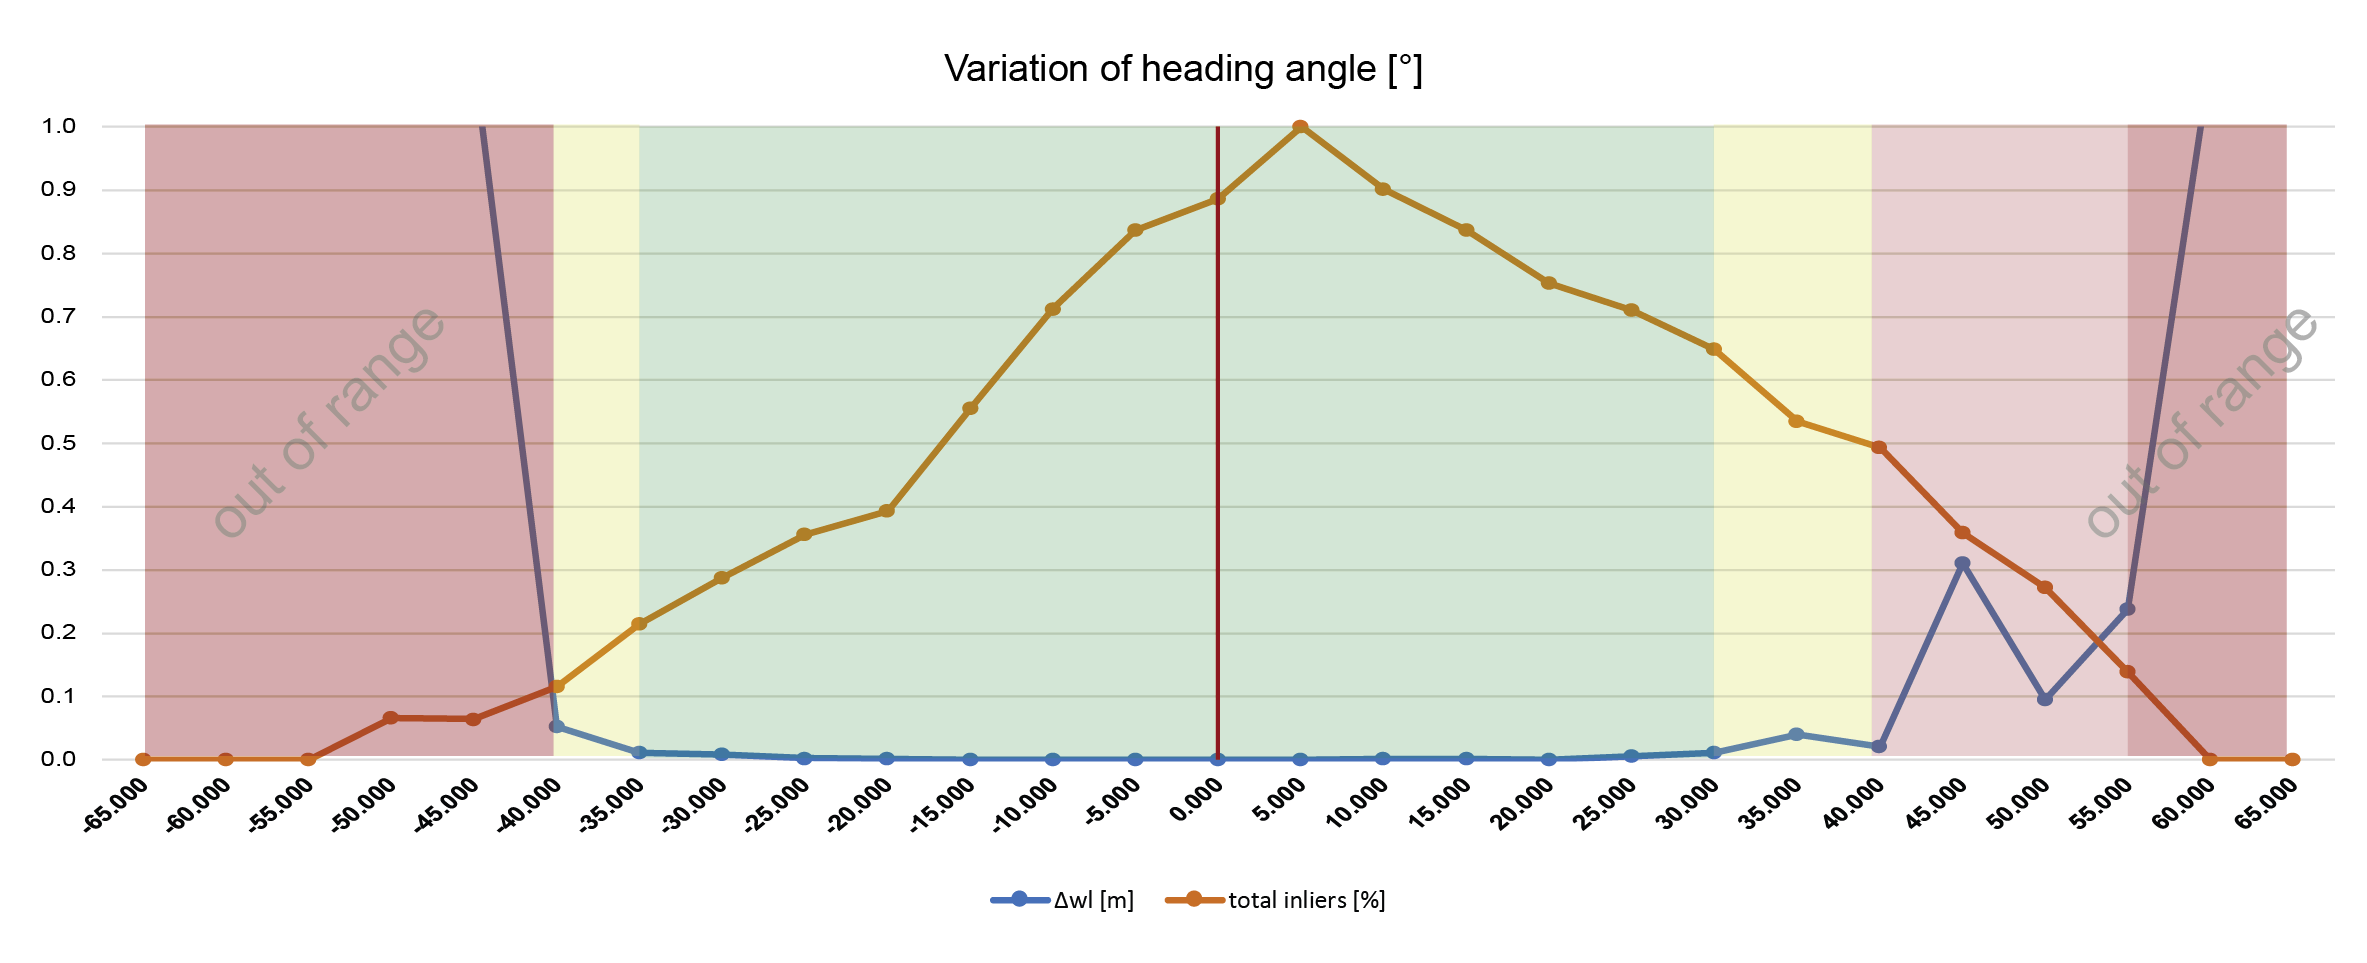
\includegraphics[keepaspectratio, width=1\columnwidth]{graphics/Sensor_Sensitivity/heading}\label{fig:sensor_sensi:heading}}
	 	\end{minipage}
	 	\begin{minipage}{\columnwidth}
	 		\centering
			\subfigure[Pitch observation]
			{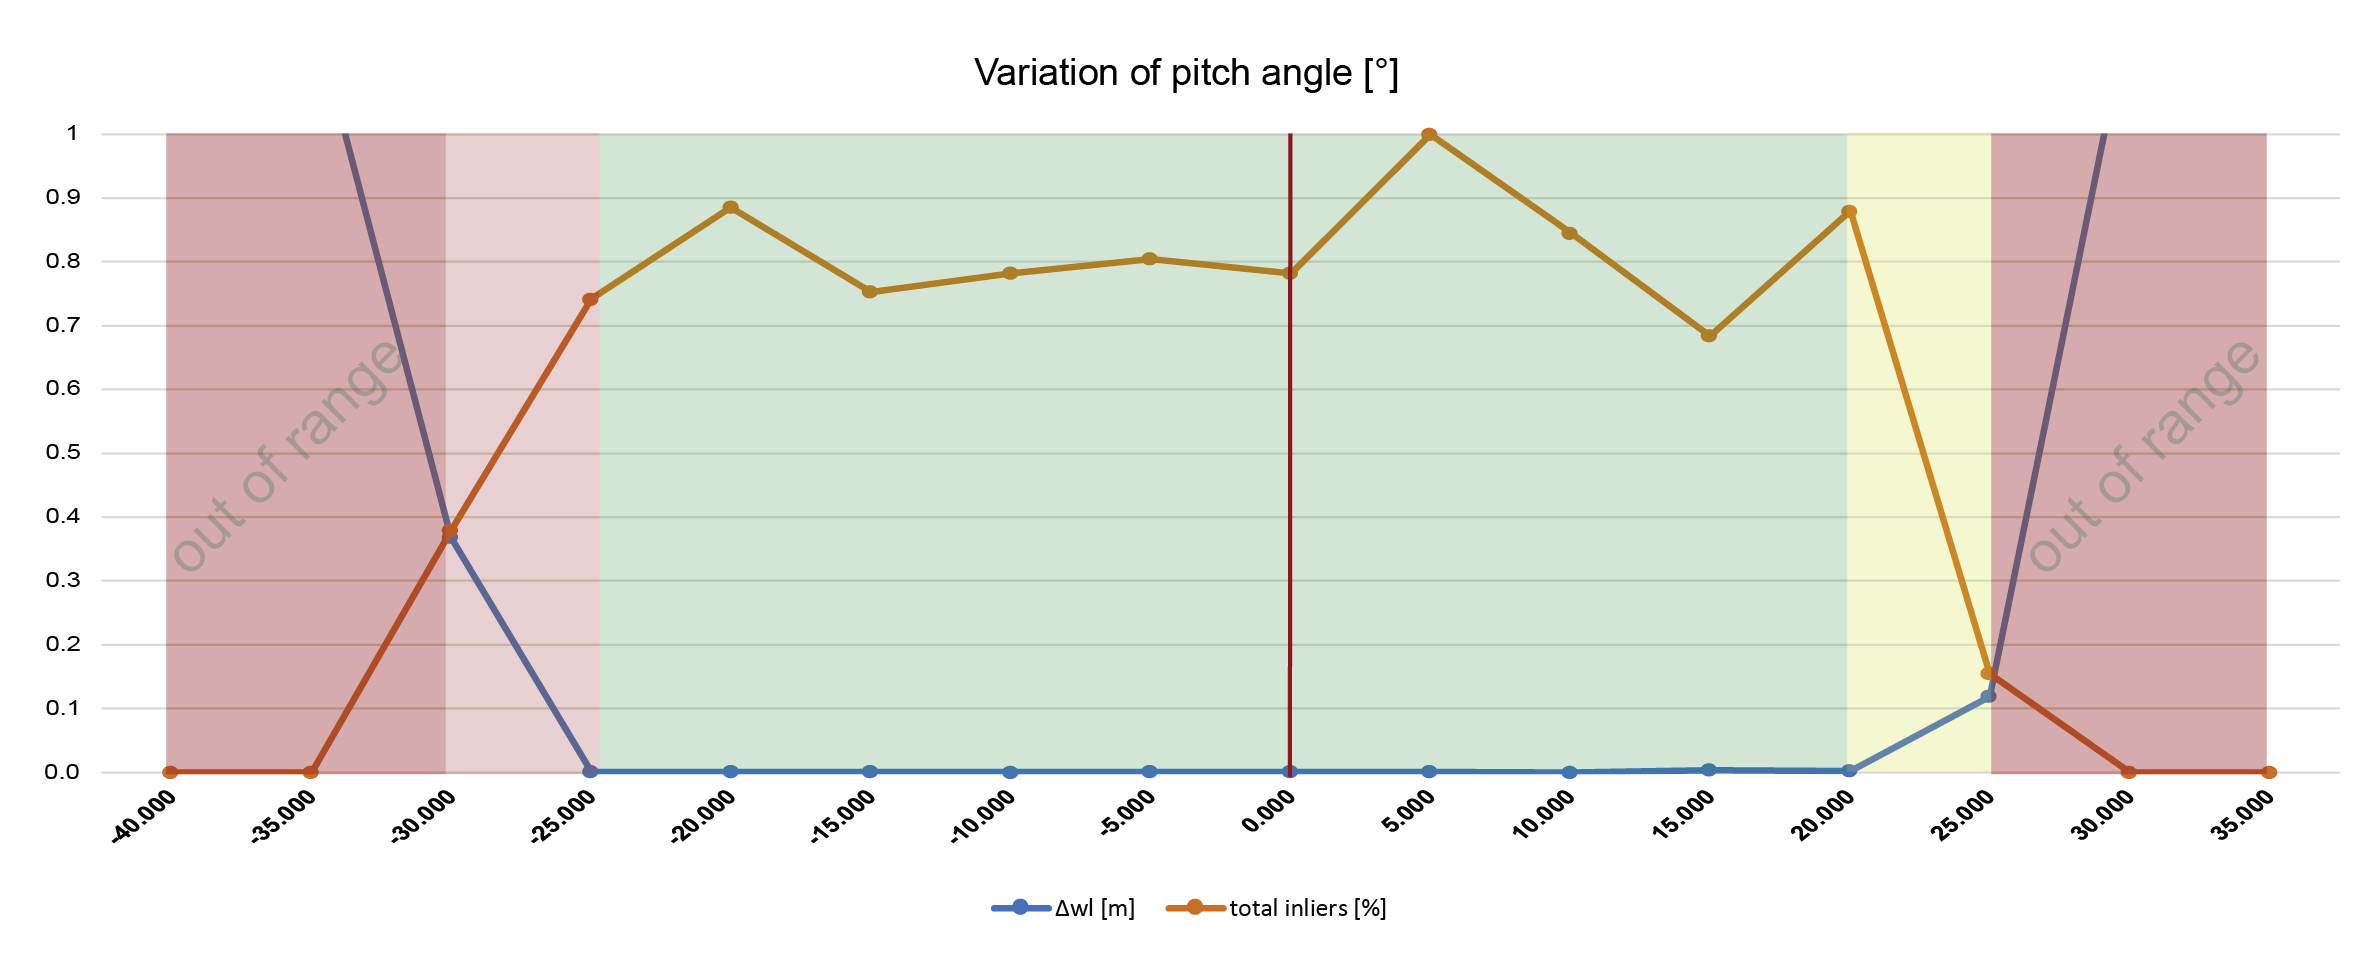
\includegraphics[keepaspectratio, width=1\columnwidth]{graphics/Sensor_Sensitivity/pitch}\label{fig:sensor_sensi:pitch}}
	 	\end{minipage}
		\begin{minipage}{\columnwidth} 
	 		\centering
			\subfigure[Roll observation]
			{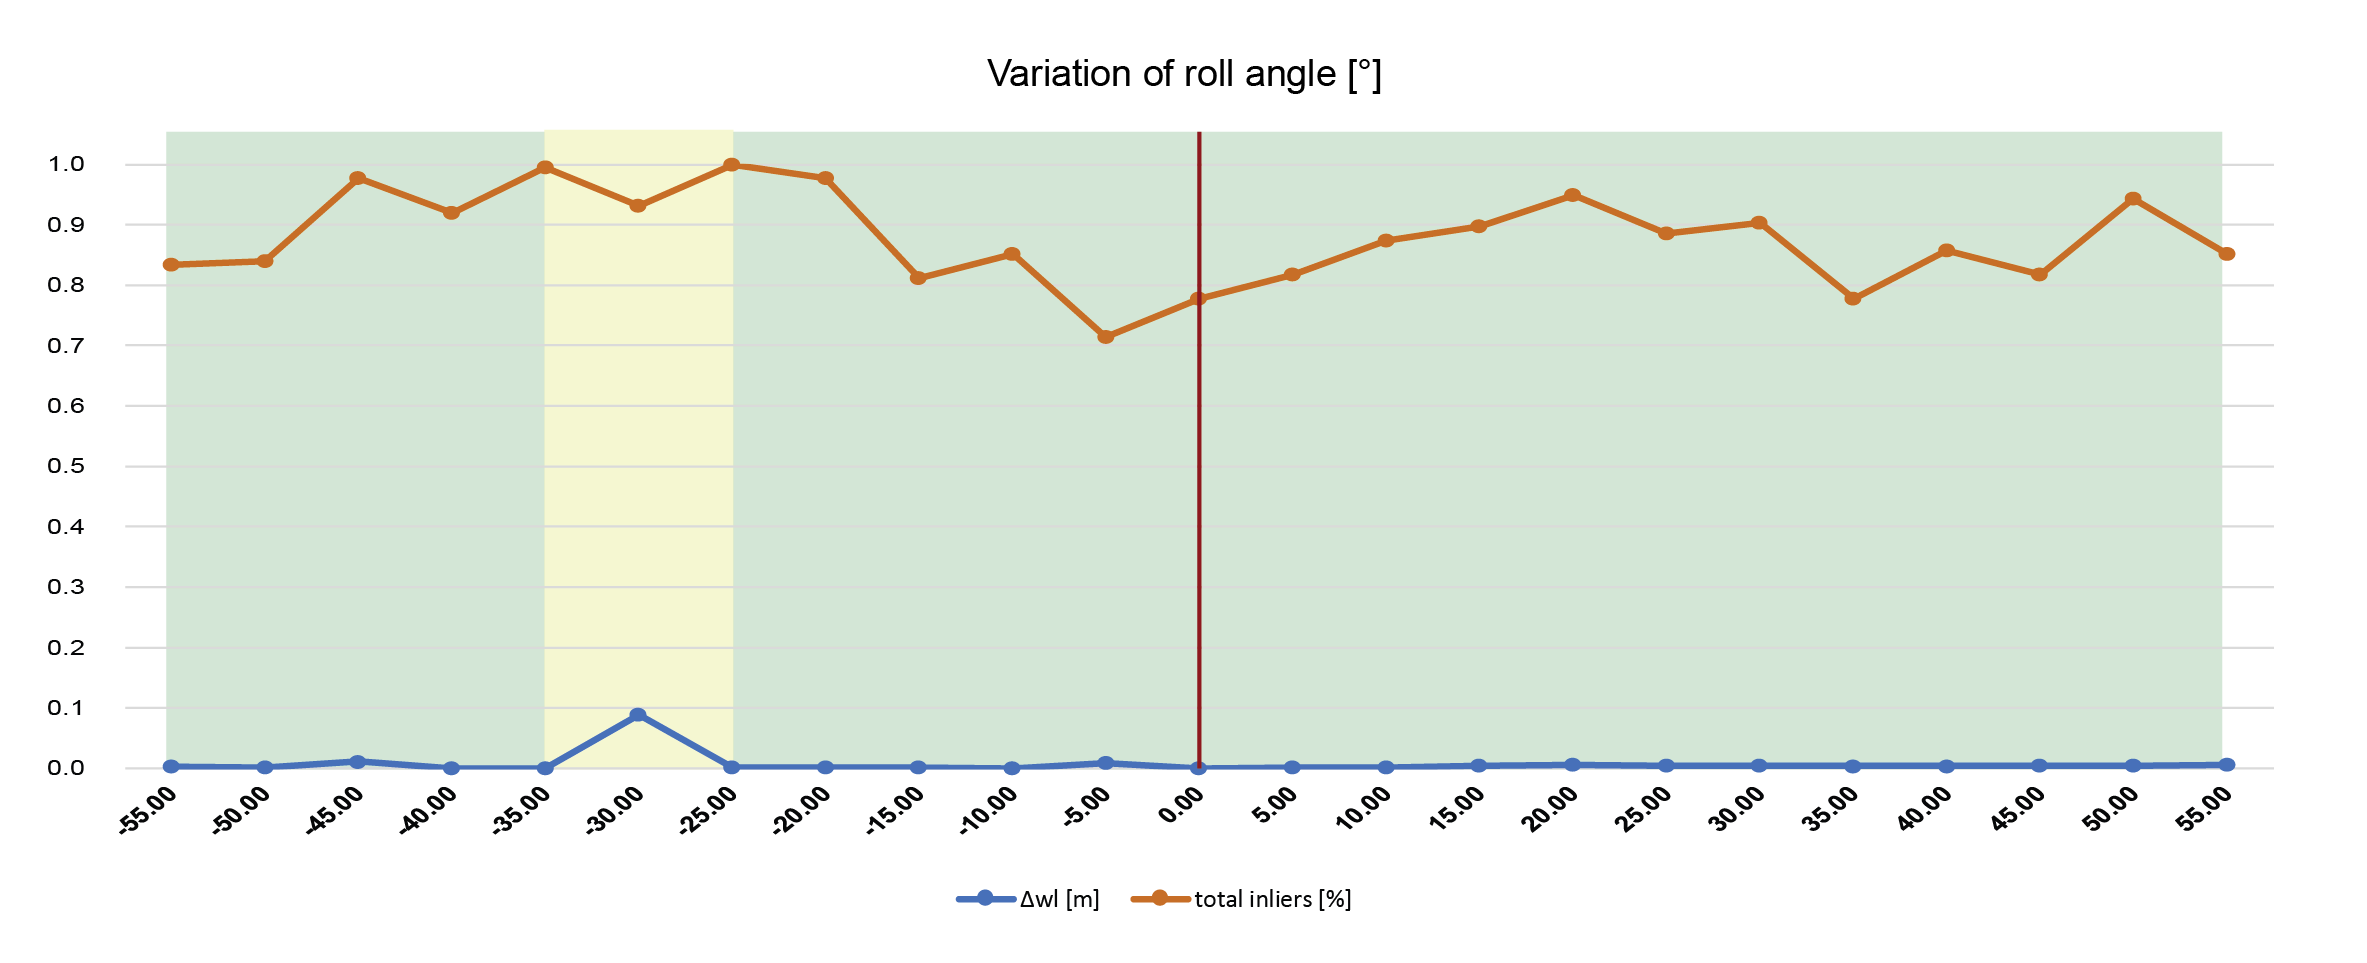
\includegraphics[keepaspectratio, width=1\columnwidth]	{graphics/Sensor_Sensitivity/roll}\label{fig:sensor_sensi:roll}}
	 	\end{minipage}
	
	\caption{Behaviour of image-2-geometry intersection depending on orientation changes. Tuning the angles heading, pitch and roll independently from each other where the others remained unchanged. ${\Delta}$wl.. absolute error for water level in meters, total inliers.. number of image features in feature-based matching displayed in percent depending on most occurrence, red/yellow/green area.. range of accuracy.}
	\label{fig:sensor_sensi}
\end{center}
\end{figure}
%[IMAGES sensor sensitivity]





\subsection{Graphics}
\label{sec:technology:graphics}

As shown in section \ref{sec:algorithms}, 3D rendering constitutes key algorithms for surface-based interpretation and annotation. Mobile devices can implement the rendering in two distinct ways: directly on the device using the integrated \gls{GPU}, or via remote rendering over the network and the transmission of images.

In cases where the app's target environment are urban settings and locations of well-developed infrastructure, the mobile device can utilise the wireless network connectivity and apply \textit{remote rendering} for the image generation. This allows externalising the rendering tasks for 3D models and supplementary data (as in Ponchio et al. \cite{Ponchio2016}), where the mobile device only submits render requests (supplemented with current view parameters) and receives the generated image. This makes the usage of larger and higher-resolution models more tangible as they are not affected by mobile device limitations. In contrast, the limitations on remote rendering are set by the requested target image size- and resolution, the target refresh rate, and the limited bandwidth of the mobile network \cite{Ponchio2016,Evans2014}. Moreover, the process is agnostic to the specific mobile device specification sending the request, making the rendering process work across all major mobile device system manufacturers (e.g. Google, Apple, Microsoft/Nokia). A positive side affect as a result of remote rendering is the reduced energy consumptions (see section \ref{sec:technology:power} for details), which allows for applying advanced algorithms for sensor tracking in localisation and orientation.

%\begin{itemize}
%% Web-Rendering - REWRITE %
%\item external circumstances and project constraints may govern implementation details for graphical systems
%\item major constraint imposed in this context is internet availability
%\item applications that are expected to operate in an urban setting or in well-developed infrastructure environments can make use of internet access
%\item this allows the externalisation of rendering tasks for 3D models and data to a network-oriented client-server architecture as in Ponchio et al. \cite{Ponchio2016}
%\item field experts that use apps and require 3D-rendered information can submit rendering requests to a remote server that takes over the image generation of the 3D data
%\item technically, the app then only transmits metadata about storage location of the 3D data and receives the final, rasterised image, which allow energy-efficient operability 
%\item furthermore, the process is agnostic to the specific mobile device generating the request, so this way of implementation works in the exact same manner for all mobile device regardless of the system manufacturer (e.g. Google, Apple, Microsoft)
%\item the reduced process load by externalising the rendering tasks allows using advanced algorithms for sensor tracking \cite{} for improved localisation and orientation or augmented reality \cite{} for information overlays and multimedia content
%% === === === ===
%\end{itemize}

The internet access may be restricted or expensive to establish (e.g. up to 70 euro per month\footnote{see \url{www.skydsl.eu}, skyDSL2+ flatrate with 30 MBit/s download}) for other outdoor applications in remote areas). Thus, outdoor applications operating in remote areas are prohibited from web-based rendering and need to perform rendering on the device. In this case, the 3D data reside in the device memory and the rendering process is affected by the performance-restricted mobile device hardware.

%see \url{www.skydsl.eu}, skyDSL2+ flatrate with 30 MBit/s download; data rate needed as high-resolution images with real-time rendering rates (uncompressed 1920x1080 pixels resolution at 30 frames/s amounts to 1.39 GBit/s) requires highest data rates

%\begin{itemize}
%\item in other geoscientific settings, such as field geology \cite{} and environmental monitoring \cite{} of remote areas, internet access is either restricted or expensive to establish
%\item subscription to satellite network with the required data rate costs around 70 euro per month \$ (see \url{www.skydsl.eu}, skyDSL2+ flatrate with 30 MBit/s download); data rate needed as high-resolution images with real-time rendering rates (uncompressed 1920x1080 pixels resolution at 30 frames/s amounts to 1.39 GBit/s) requires highest data rates even when employing advanced compression techniques
%\item thus, for geoscience applications that operate in remote areas, web-based rendering is not an option
%\item in these cases, rendering needs to be done on the device
%\item for on-device rendering, the 3D data need to reside in the device memory and image generation needs to be done with performance-restricted hardware
%\end{itemize}

% === === Leave out as really not too relevant the way it is written === === %
%% software- vs hardware renderer
%\begin{itemize}
%\item as explained above, rendering 3D data is a key part for conducting annotations on 3D data, either based on 3D geometry itself or correlated images in camera space
%\item for mobile devices, this can technologically be realized two-fold, depending on the usage constraints
%\item generally, rendering stages (image-place projection, rasterization, tesselation \& lighting, see \cite{Kessenich2016}) can be realised by means of software or by hardware support
%\item here, compute operations (gaussian smoothing, derivative computations, vertex projection) are implemented on the mobile device CPU by available operations and libraries using the Android SDK (Java) and Android NDK (C++) on Google's Android system and Swift and Objective-C on Apple's iOS platform
%\item software-based rendering is more flexible in how operations are carried out as they do not need to account for hardware-specific processing pipelines; in the realm of mobile devices, non-standard software-based rendering operations are supported by a wider range of devices
%\item drawback of software-based rendering is performance as it makes suboptimal use newer computing capabilities and graphics-specific chipset operations
%\item example is the novel rendering approach for point-based rendering introduced in section \ref{}, which requires implementation flexibility
%\item most 3D rendering is done, even on mobile devices, with hardware-based rendering to varying degrees
%\item even when implementing specific rasterization algorithms (see section \ref{}), operations such as vertex projections and tesselation \& lighting are performed on the GPU
%\item hardware-based rendering on mobile devices is facilitated by Khronos' \gls{GLES} \cite{Mehta2013} on specialised mobile device graphics chips (e.g. Qualcomm Adreno, ARM Mali, NVIDIA Tegra)
%\item in comparison to software-based rendering, hardware acceleration provides improved performance
%\item drawbacks of hardware implementations are considerably longer development cycles, because the programming principles of GPUs differ considerably from common ''App programming´´, and reduced flexibility on what can be realised
%\item for geoscientists and domain experts in the field, the distinction is good to be aware of as accelerated graphical apps for solving domain-specific tasks are usually offered as paid services to offset the increased development costs
%\end{itemize}

The emergence of mobile graphics libraries such as Khronos \gls{GLES}, Vulcan and Open Scene Graph on Android\footnote{osgAndroid - original at \url{https://github.com/miragetech/osgAndroid}, extended by the second author at \url{https://github.com/CKehl/osgAndroid}}, as well as the continuously improving mobile graphics chipsets (e.g. Qualcomm Adreno, ARM Mali, NVIDIA Tegra), makes on-device rendering a feasible option for apps targeting field-based geosciences. Pinhead example software for field-based studies using mobile device graphics on some way are OpenWaterLevel \cite{Kroehnert2017a}, \gls{GRIT} \cite{Kehl2016_VGCabstract} and Outcrop \cite{Viseur2014_VGCabstract}. Mobile graphics itself is still a hot topic with is the principle science discipline of computer graphics, visualisation and virtual reality \cite{Rodriguez2012,Rodriguez2014,Garcia2015,Agus2017}. Scaling up the principle graphics lab results (in terms of data size, image resolution and texture utilisation), often demonstrated on small-extent individual objects in cultural heritage, to actual requirements within the geosciences is a prime challenge. Although mobile manufacturers provide more powerful devices to allow for more data and higher resolutions, mobile devices need to sacrifice capabilities such as sensor availability as well as physical size and weight in order to provide larger memory space and higher-performance processors. Examples for this trade-off manufacturing can be seen in special-purpose and high-performance tablets such as NVIDIA Shield\footnote{NVIDIA Shield - \url{https://developer.nvidia.com/develop4shield}}, Project Tango resp. ARCore\footnote{Google Augmented Reality - \url{https://developers.google.com/ar/}} and Google Pixel C\footnote{Google Pixel C- \url{https://www.android.com/tablets/pixel-c/}}. Another problem rarely considered in scientific literature on mobile graphics is power consumption, which is of pivot importance for field practitioners (see section \ref{sec:technology:power}). A specific problem that impacts geoscientists and domain experts with respect to on-device rendering settings is the trade-off between app responsiveness, image quality, hardware utilization and cross-device operability illustrated in fig. \ref{fig:technology:graphics:imagingTrinity}.

\begin{figure}[h]
\centering
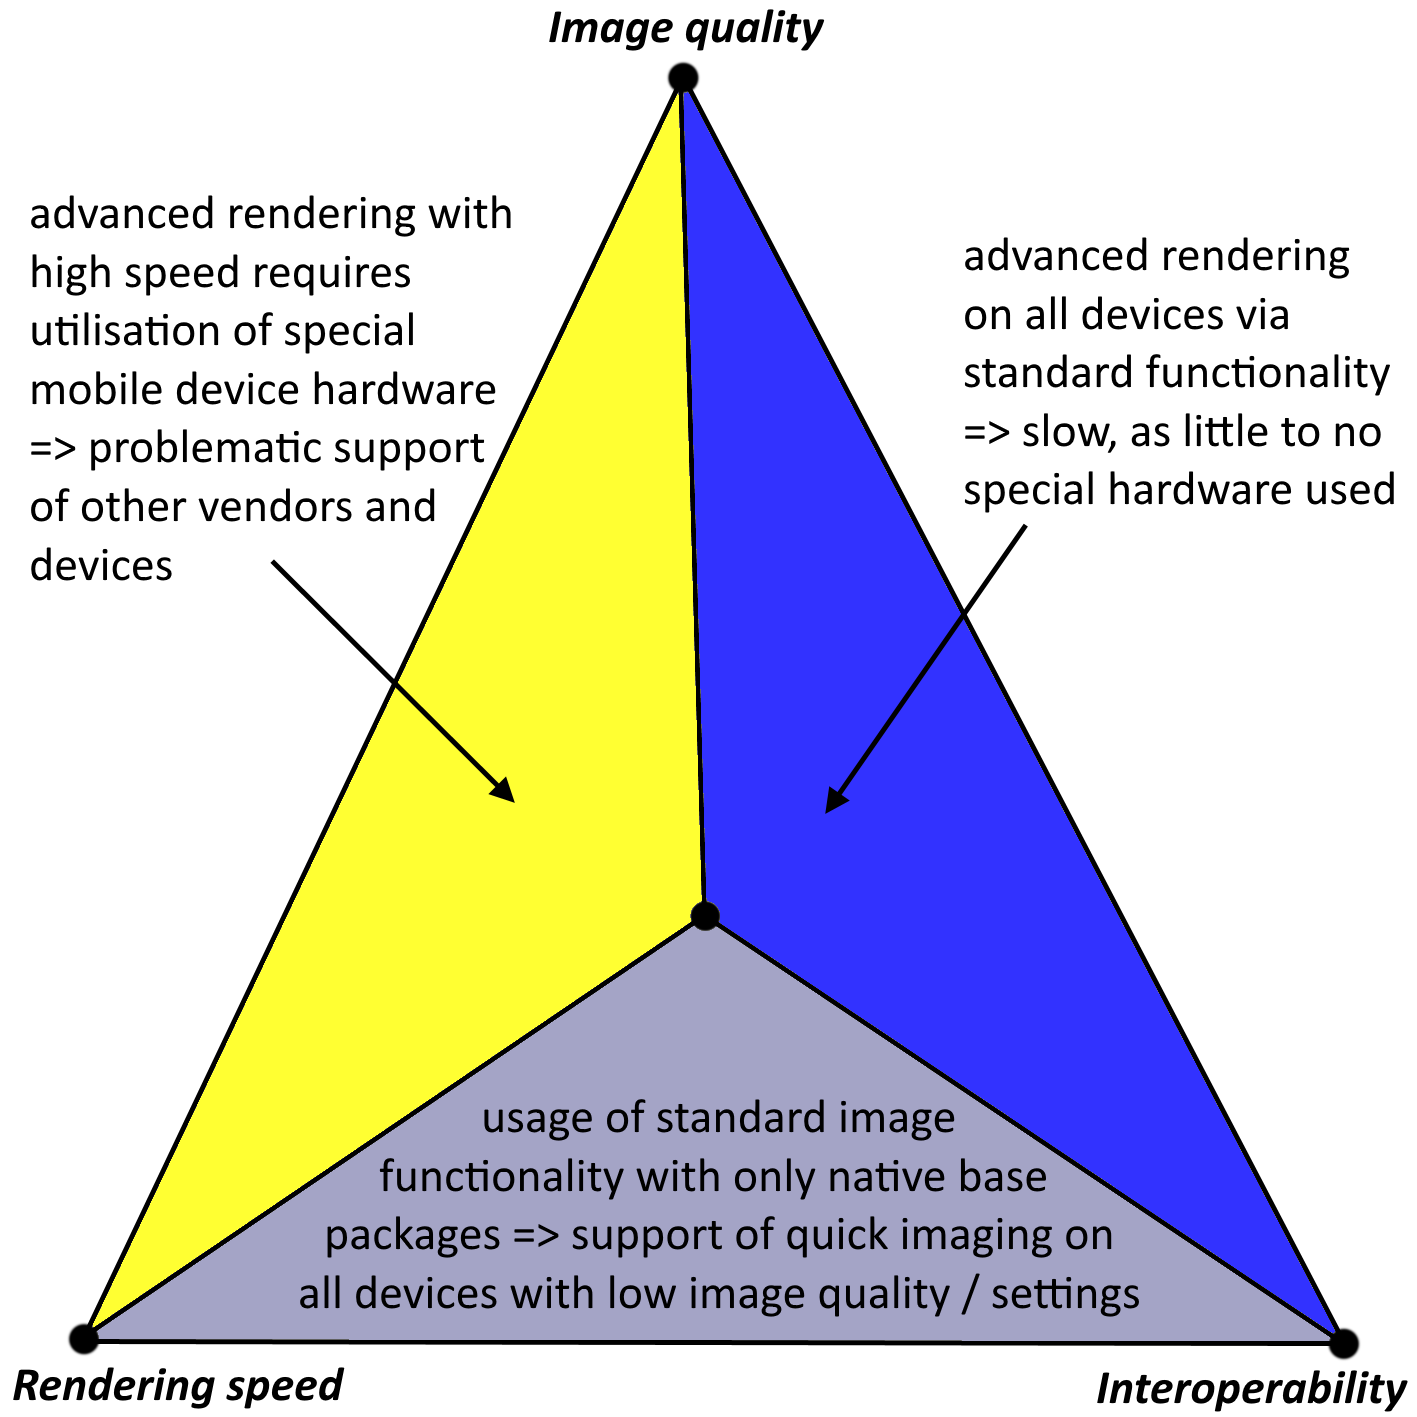
\includegraphics[width=0.75\columnwidth]{graphics/ImagingTrinity}
\caption{Conflicting trinity of image (i.e. rendering) quality, rendering speed (a collective term is this context for special hardware utilisation and responsiveness) and interoperability (between devices of the same vendor as well as between vendors).}
\label{fig:technology:graphics:imagingTrinity}
\end{figure}
%[triangle of the Trinity of Image Quality, Rendering Speed (=hardware utilization+responsiveness) and Interoperability]

%\begin{itemize}
% === === Rendering-on-Device === === %
%\item as is shown in section \ref{}, on-device rendering has considerable impact on the energy consumption
%\item on-device rendering that processes realistic field data requires considerable implementation efforts, as demonstrated by apps such as OpenWaterLevel \cite{}, GRIT \cite{Kehl2016_VGCabstract} and Outcrop \cite{Viseur2014_VGCabstract}
%\item principle scientific advances in mobile device rendering have demonstrated considerable progress over the years \cite{Garcia2015,Kehl2015c,Agus2017}
%\item scaling up smaller laboratory results with mobile graphics to realistic geoscience data, in terms of image quality and resolution as well as 3D base data, is a persisting challenge
%\item although technical development continuously provides more powerful devices, mobile devices need to sacrifice capabilities such as sensor availability as well as physical size and weight in order to provide larger memory space and higher-performance processors; examples for this trade-off manufacturing can be seen in special-purpose and high-performance tablets such as NVIDIA Shield\footnote{NVIDIA Shield - \url{https://developer.nvidia.com/develop4shield}}, Project Tango resp. ARCore\footnote{Google Augmented Reality - \url{https://developers.google.com/ar/}} and Google Pixel C\footnote{Google Pixel C- \url{https://www.android.com/tablets/pixel-c/}}
%\end{itemize}

In interviews conducted amongst field geologists at the dept. of earth science at the university of Bergen, a major demand by the target user base (i.e. domain experts and practitioners) of such mobile app is the interoperability between Android, Microsoft and Apple devices. This demand possibly originates from the platform-agnostic functioning of common geoscience software (e.g. \glspl{GIS}, geomodelling software) on desktop computers for Apple and Windows. On the other hand, app responsiveness and high image quality are amongst the next common priorities behind interoperability. Moreover, the interviewed geoscientists expect to receive visibly improved image quality- or functionality when advanced equipment (e.g. special-purpose tablets, novel- and high-performance tablets) is available. Both demands are conflicting because making use of specialised hardware (e.g. \gls{GPU} Computing such as CUDA\footnote{CUDA - \url{https://developer.nvidia.com/cuda-zone}} for image processing \cite{Heymann2007,Hudelist2014}, texture compression \cite{Chait2015}) in turn means reducing the range of devices being able to operate the software. Still, these specialised technologies are key to achieve the required responsiveness and image quality.

%\begin{itemize}
% === === hardware differences: speed, capability, CUDA === === %
%\item an specific problem for geoscientists and domain experts in on-device rendering settings: trade-off between app response time, image quality, hardware utilization and cross-device operability
%\item in interviews amongst field geologists at the department of earth science at university of Bergen, a major demand from the target user base of such mobile app is interoperability between Android, Microsoft and Apple devices; demand originates from platform-agnostic working of common geoscience software on desktop computers for Apple and Windows
%\item on the other hand, app responsiveness and high image quality are amongst the next common priorities behind interoperability; user base asks for improved quality when operating advanced equipment (e.g. special-pirpose tablets, novel- and high-performance tablets)
%\item both demands are conflicting, as making use of specialised hardware (e.g. 64-bit, \gls{SSE} and vectorisation, parallel processing and \gls{GPU} Computing such as CUDA\footnote{CUDA - \url{https://developer.nvidia.com/cuda-zone}} for image processing \cite{Heymann2007,Hudelist2014}, texture compression \cite{Chait2015}) in turn means reducing the range of devices being able to operate the software
%\item these technologies are key as they provide technical solutions available right now to achieve the required responsiveness and image quality
%\end{itemize}

%\subsection{Component differences between devices}
%
%\begin{itemize}
%\item camera
%\end{itemize}

\subsection{Power consumption}
\label{sec:technology:power}

Power consumption is an important metric for mobile field applications, which is at the same time also distinct to the mobile device platform. This metric governs the operation time of an app in an outdoor field setting for specific studies. In application domains such as field geology, the target operation time is in the range of four hours to eight hours without device recharging. The original operation time can be extended with external battery packs, although there is a limit of how many battery packs can be taken into the field before their total weight renders the mobile device impractical as a field tool.

We measured the energy consumption of \textit{Open Water Level} and \textit{\gls{GRIT}} in realistic settings for case studies in waterline detection and field interpretation. Measuring the power consumption on an app-specific level is not supported by default on mobile devices. Formerly, the power consumption has only been assessed on a hardware component level \cite{Carroll2010}. This study utilised the Trepn Profiler \footnote{Trepn Profiler - \url{https://developer.qualcomm.com/software/trepn-power-profiler}}, which is currently the only known app on Android devices that facilitate app-specific measurements. Trepn Profiler also allows for the simultaneous logging of technical indicators (e.g. \gls{GPU}- and \gls{CPU} load, memory consumption, \gls{CPU} temperature), which is used in this study to draw higher-level conclusions on the utilisation of the apps. The presented measurements were obtained on a Google Nexus 5 smartphone (4-core ARM \gls{CPU}, Qualcomm Adreno \gls{GPU}). Additional measurements have been obtained with a Samsung S8 (8-core ARM \gls{CPU}, ARM Mali \gls{GPU}), which can be located in the supplementary data of this article.

%\begin{itemize}
%\item power consumption is a metric of major importance for mobile field applications
%\item metric governs the operation time of an app outdoors for specific studies; in application domains such as field geology, the target operation time is in the range of four to eight hours without recharging at an electricity plug
%\item for the use cases of waterline detection and field interpretation, we measured the energy consumption of the apps ''OpenWaterLevel'' and ''GRIT'' and its relation to technical indicators, such as \gls{CPU}- and \gls{GPU} utilisation, memory consumption and environment measures that influence chip operations, namely the processor temperature
%\item the following measures for both apps were obtained on a Google Nexus 5 smartphone with 4-core ARM Cortex \gls{CPU} and Qualcomm Adreno \gls{GPU}; furthermore, OpenWaterLevels and its \gls{CPU}-related measures were validated on a Samsung S8 smartphone with an 8-core ARM Cortex \gls{CPU} of newer generation
%\item currently, the only app available on Android that allows measuring metrics on an app-specific level (i.e. logging the power consumption related to just one specific external app) is the Trepn Profiler \footnote{Trepn Profiler - \url{}}
%\item while this profiling app runs on all Android devices, the metrics that can be recorded (e.g. \gls{GPU} load, processor temperature) vary between devices, so that \gls{GPU} load measurements are not available for the Samsung S8 smartphone
%\item also the reason why measurements have been carried out on Google smartphones instead of other tablets; general insight on processor-power consumption behaviour are possible to be extrapolated to other devices
%\end{itemize}

In an initial test, we compare the power consumption relative to the \gls{CPU}- and \gls{GPU} load. Our initial hypothesis was that a higher \gls{GPU} load results in an increased power consumption compared to \gls{CPU}-dominated operations, because mobile \glspl{GPU} draw more power than \glspl{CPU} to realise the increased graphics performance. The results are shown for \gls{GRIT} and for OpenWaterLevel, split in \gls{CPU} (fig. \ref{fig:power:CPU_2D_contrast}) and \gls{GPU} (fig. \ref{fig:power:GPU_2D_contrast}) contributions.

\begin{figure}[htbp!]
\begin{center}
	 	\begin{minipage}{\columnwidth}
	 		\centering
			\subfigure[Open Water Levels]
			{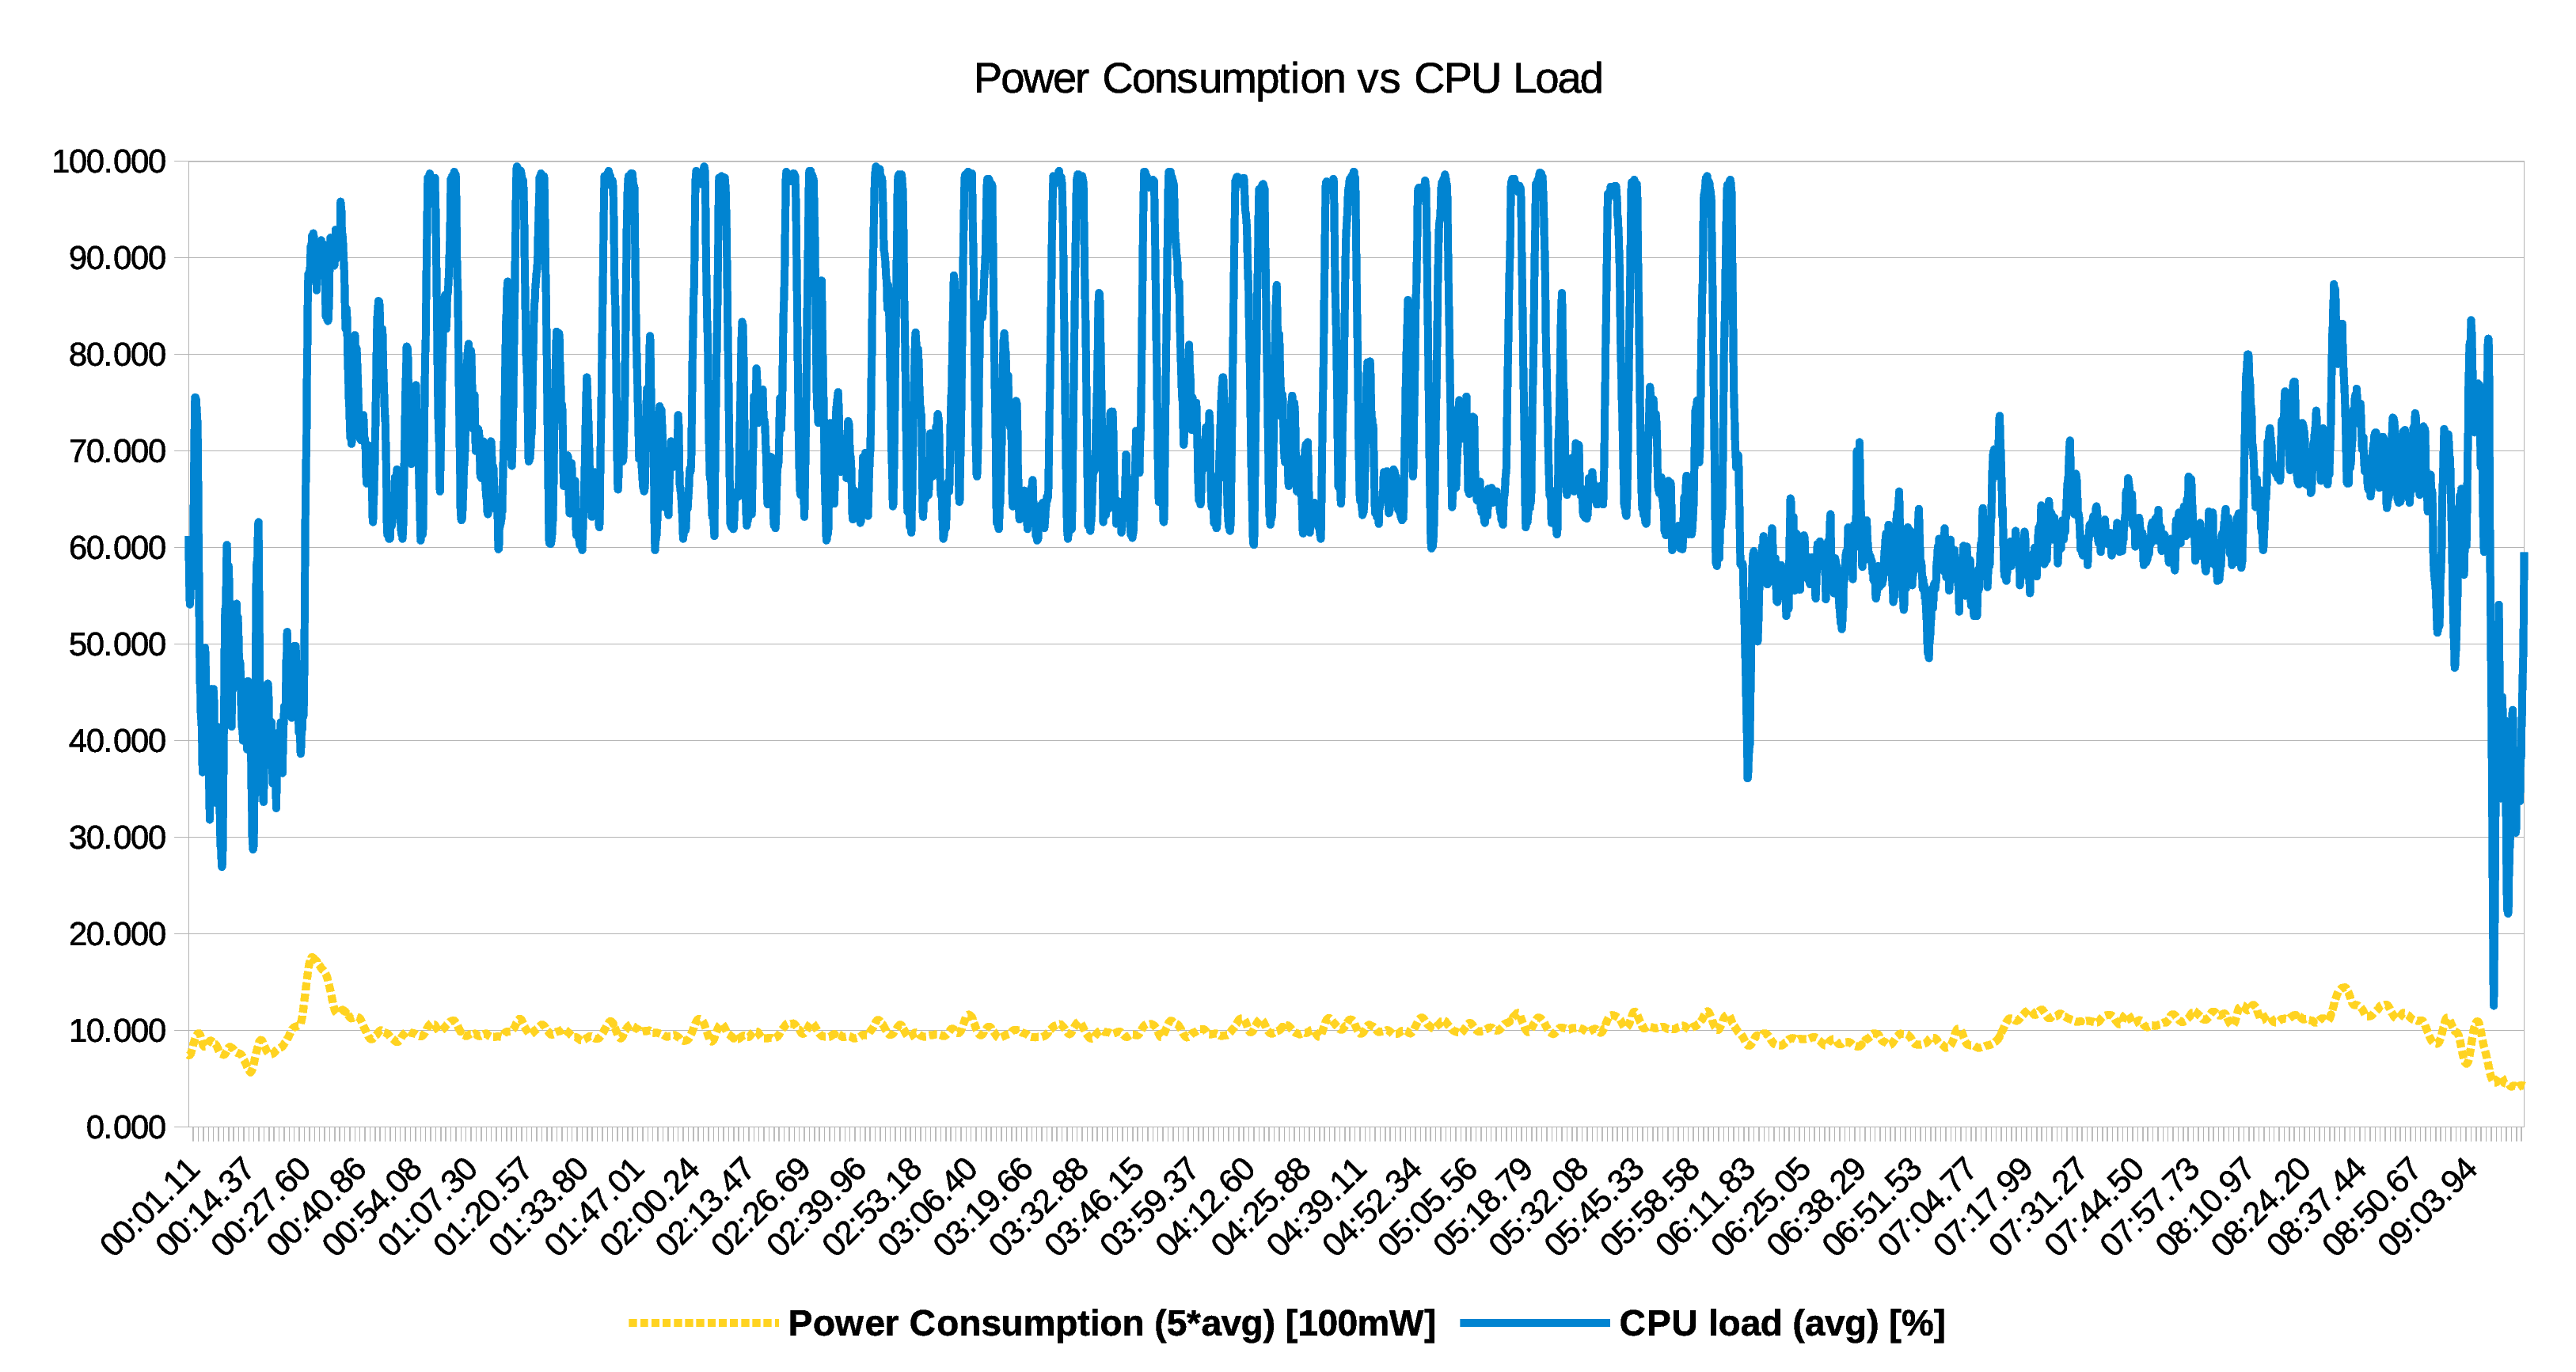
\includegraphics[keepaspectratio, width=0.95\columnwidth]{graphics/OWL_Nexus5/Power_CPU_run2}\label{fig:power:CPU_2D_contrast:OWL}}
	 	\end{minipage}
	 	\begin{minipage}{\columnwidth}
	 		\centering
			\subfigure[GRIT]
			{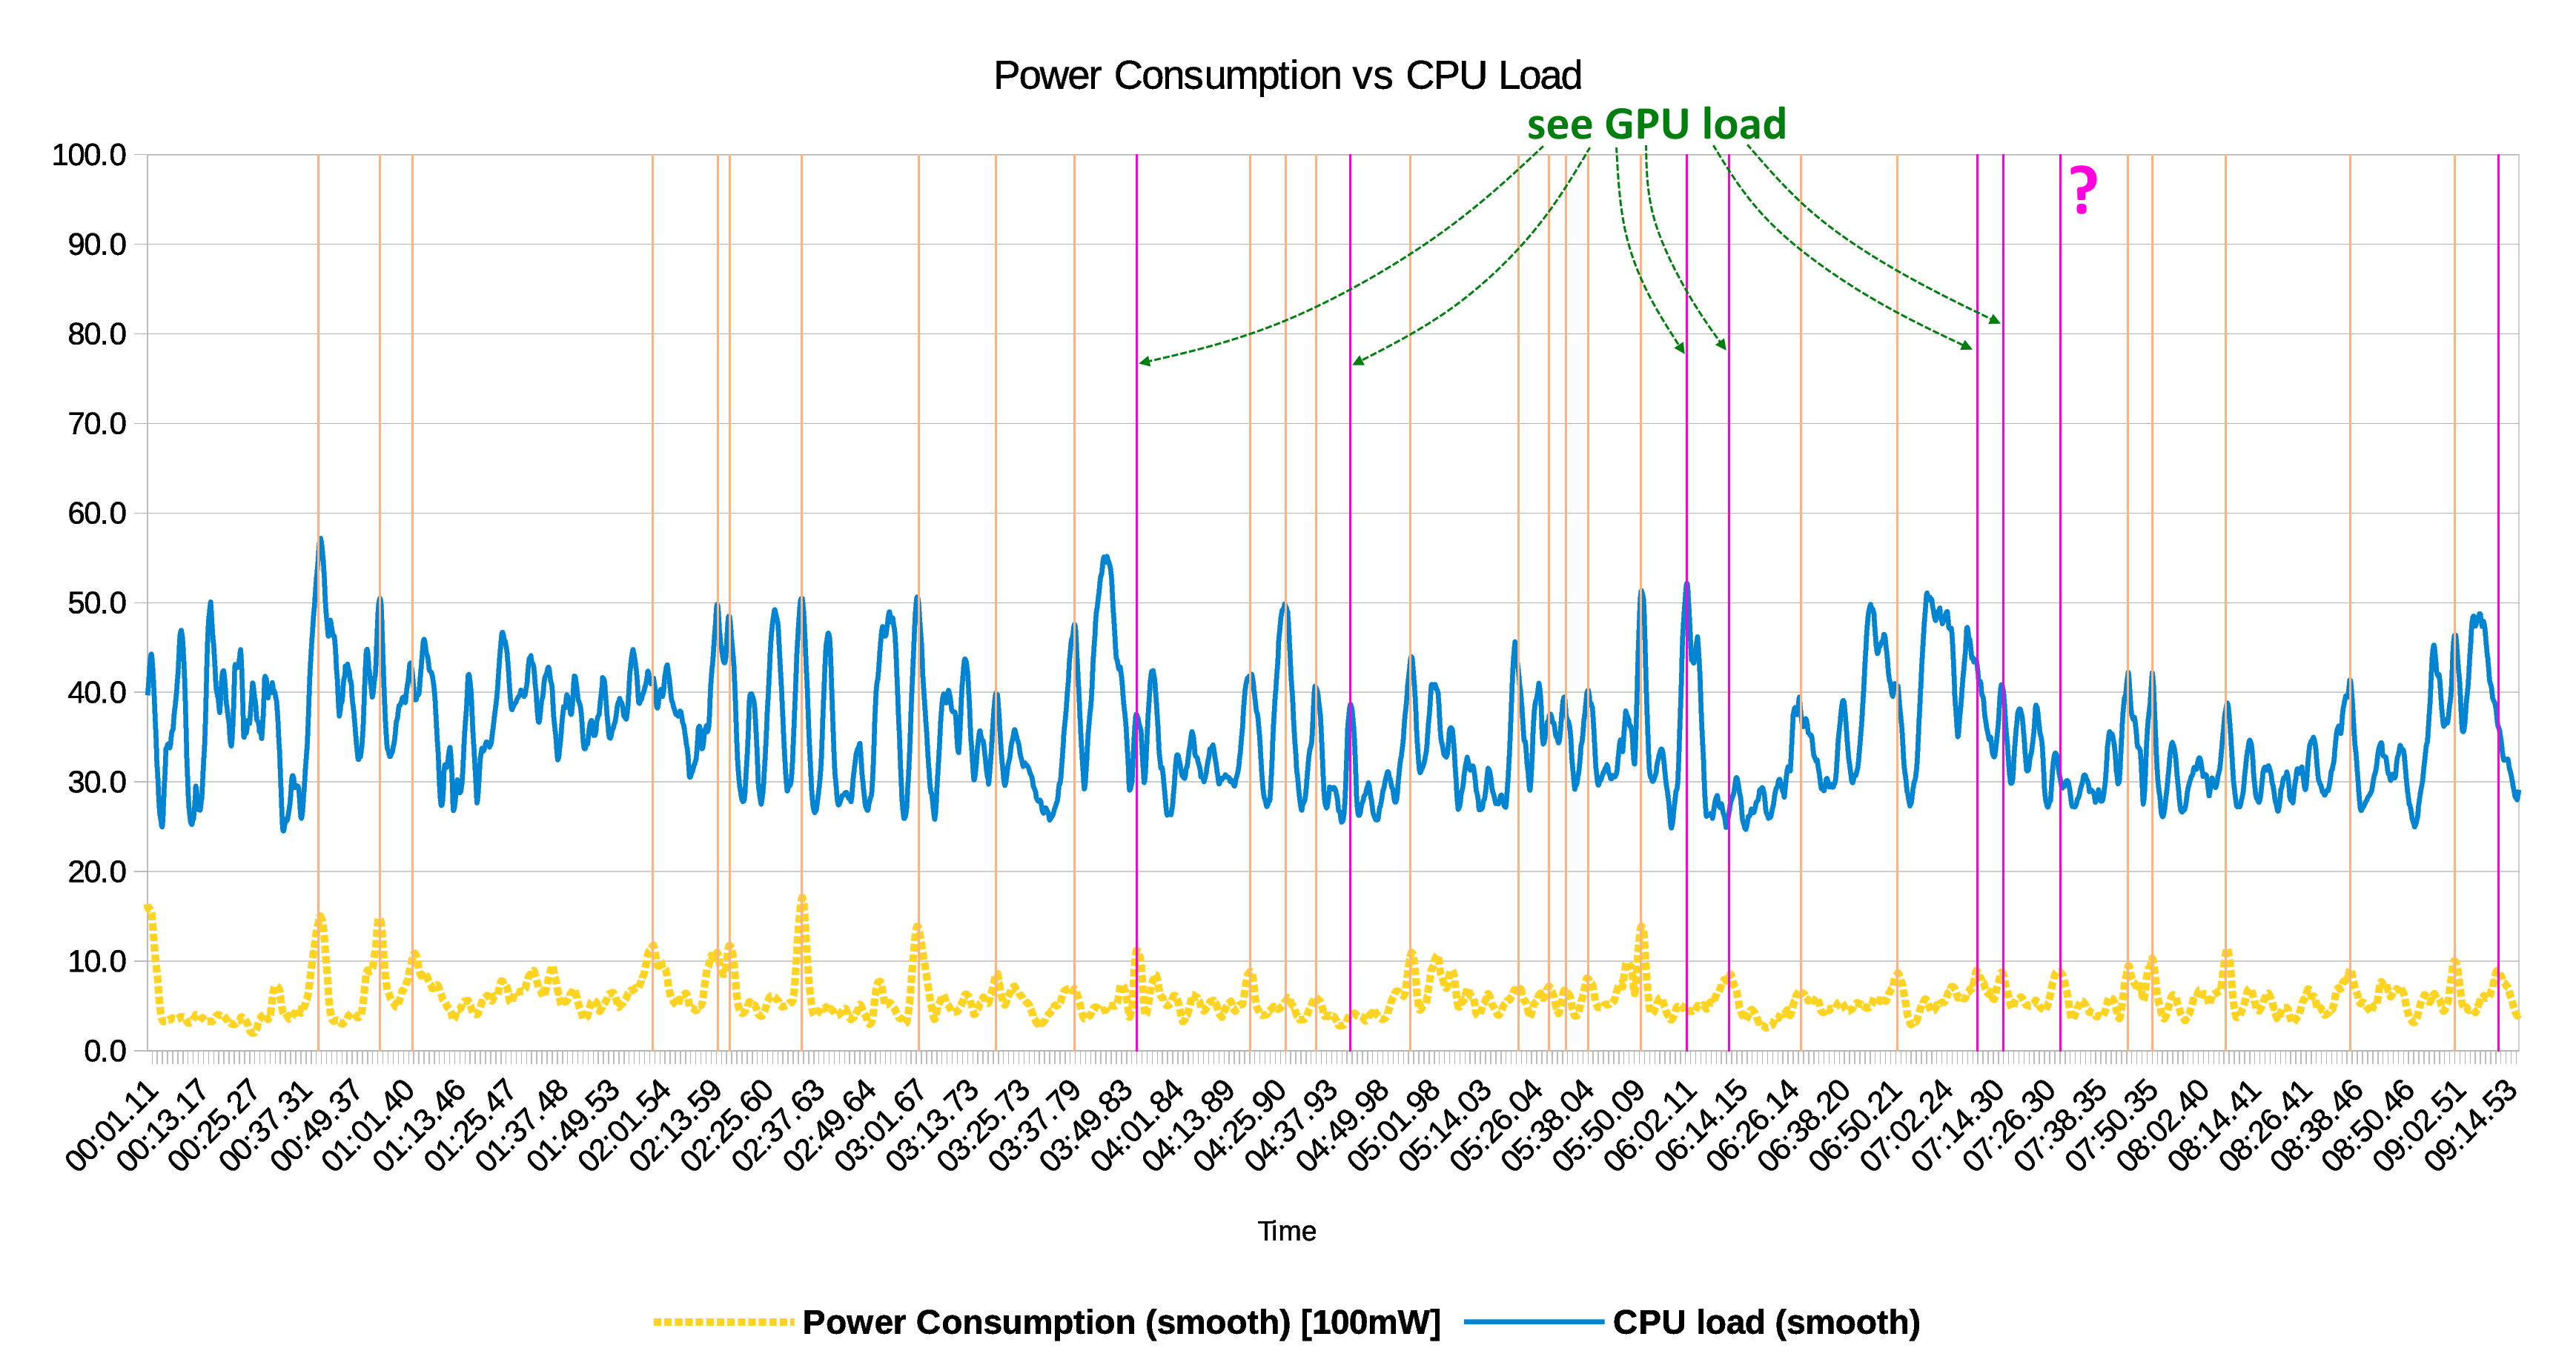
\includegraphics[keepaspectratio, width=0.95\columnwidth]{graphics/GRIT/Measure2D_Power_CPU}\label{fig:power:CPU_2D_contrast:GRIT}}
	 	\end{minipage}
	\caption{Diagram of power measurements with respect to the CPU load, comparing Open Water Levels and GRIT in 2D mode. The less saturated lines show direct correlations between peak CPU load and peak power consumption, while fully saturated lines show missing peak correlations where they are expected.}
	\label{fig:power:CPU_2D_contrast}
\end{center}
\end{figure}
%[IMAGES power vs CPU]

\begin{figure}[htbp!]
\begin{center}
	 	\begin{minipage}{\columnwidth}
	 		\centering
			\subfigure[Open Water Levels]
			{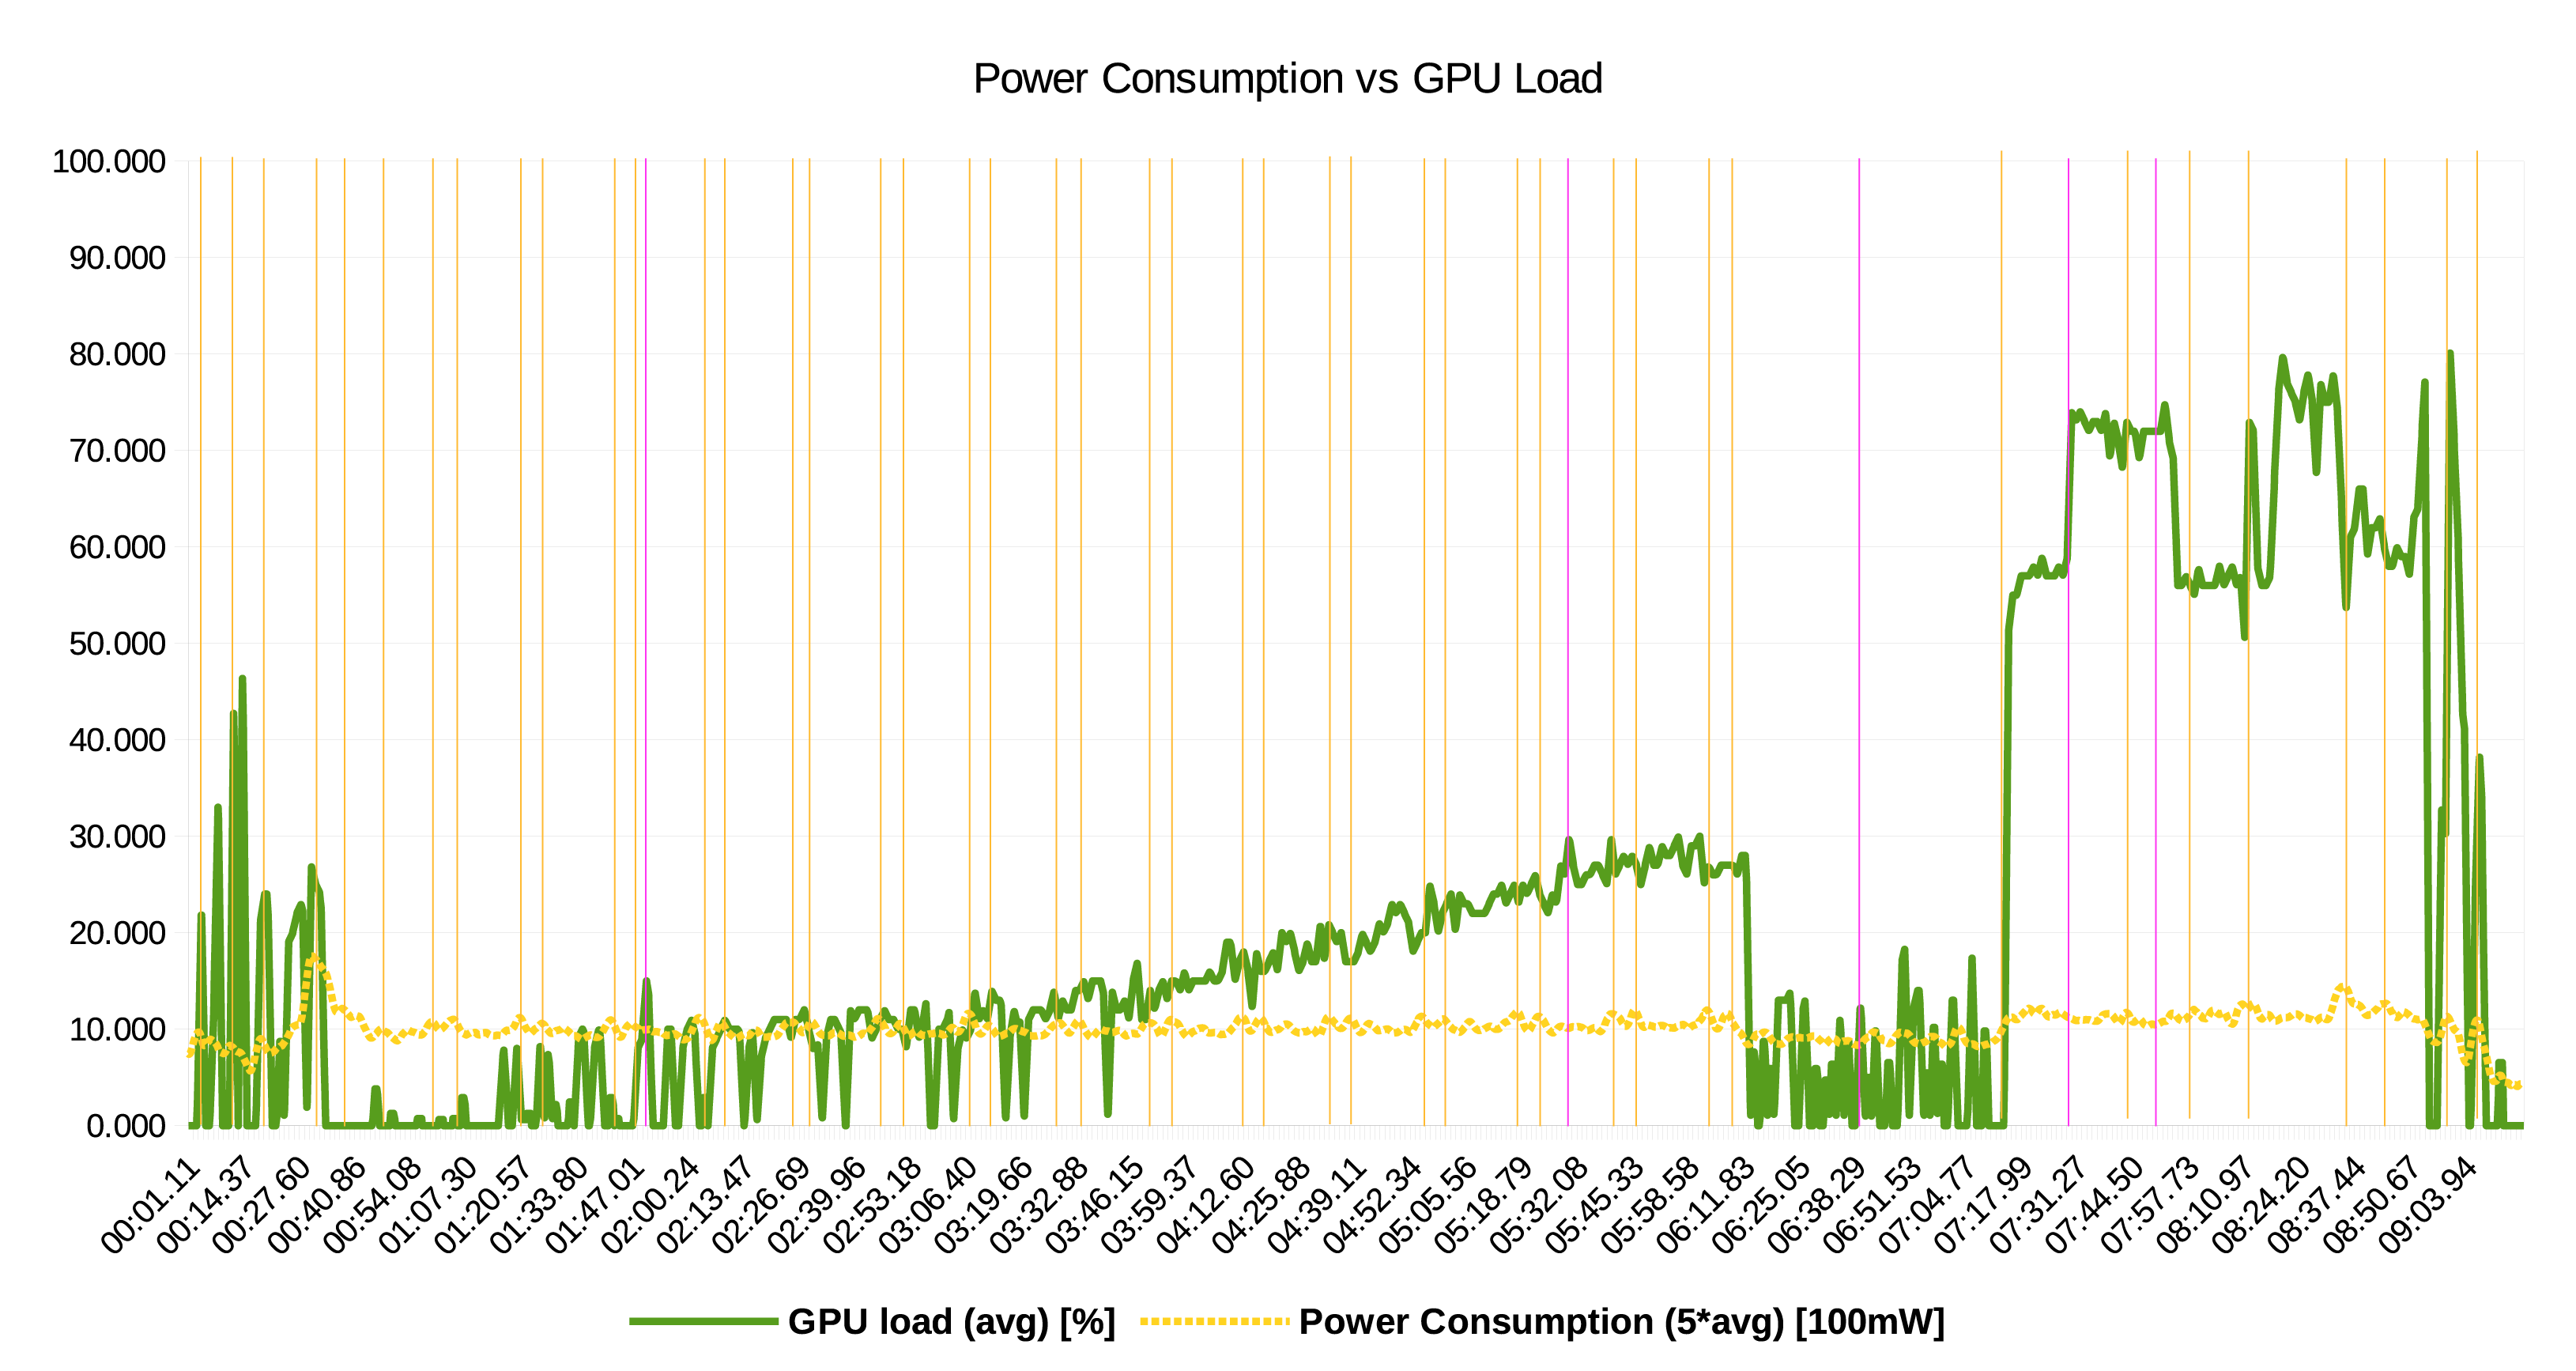
\includegraphics[keepaspectratio, width=0.95\columnwidth]{graphics/OWL_Nexus5/Power_GPU_run2}\label{fig:power:GPU_2D_contrast:OWL}}
	 	\end{minipage}
	 	\begin{minipage}{\columnwidth}
	 		\centering
			\subfigure[GRIT]
			{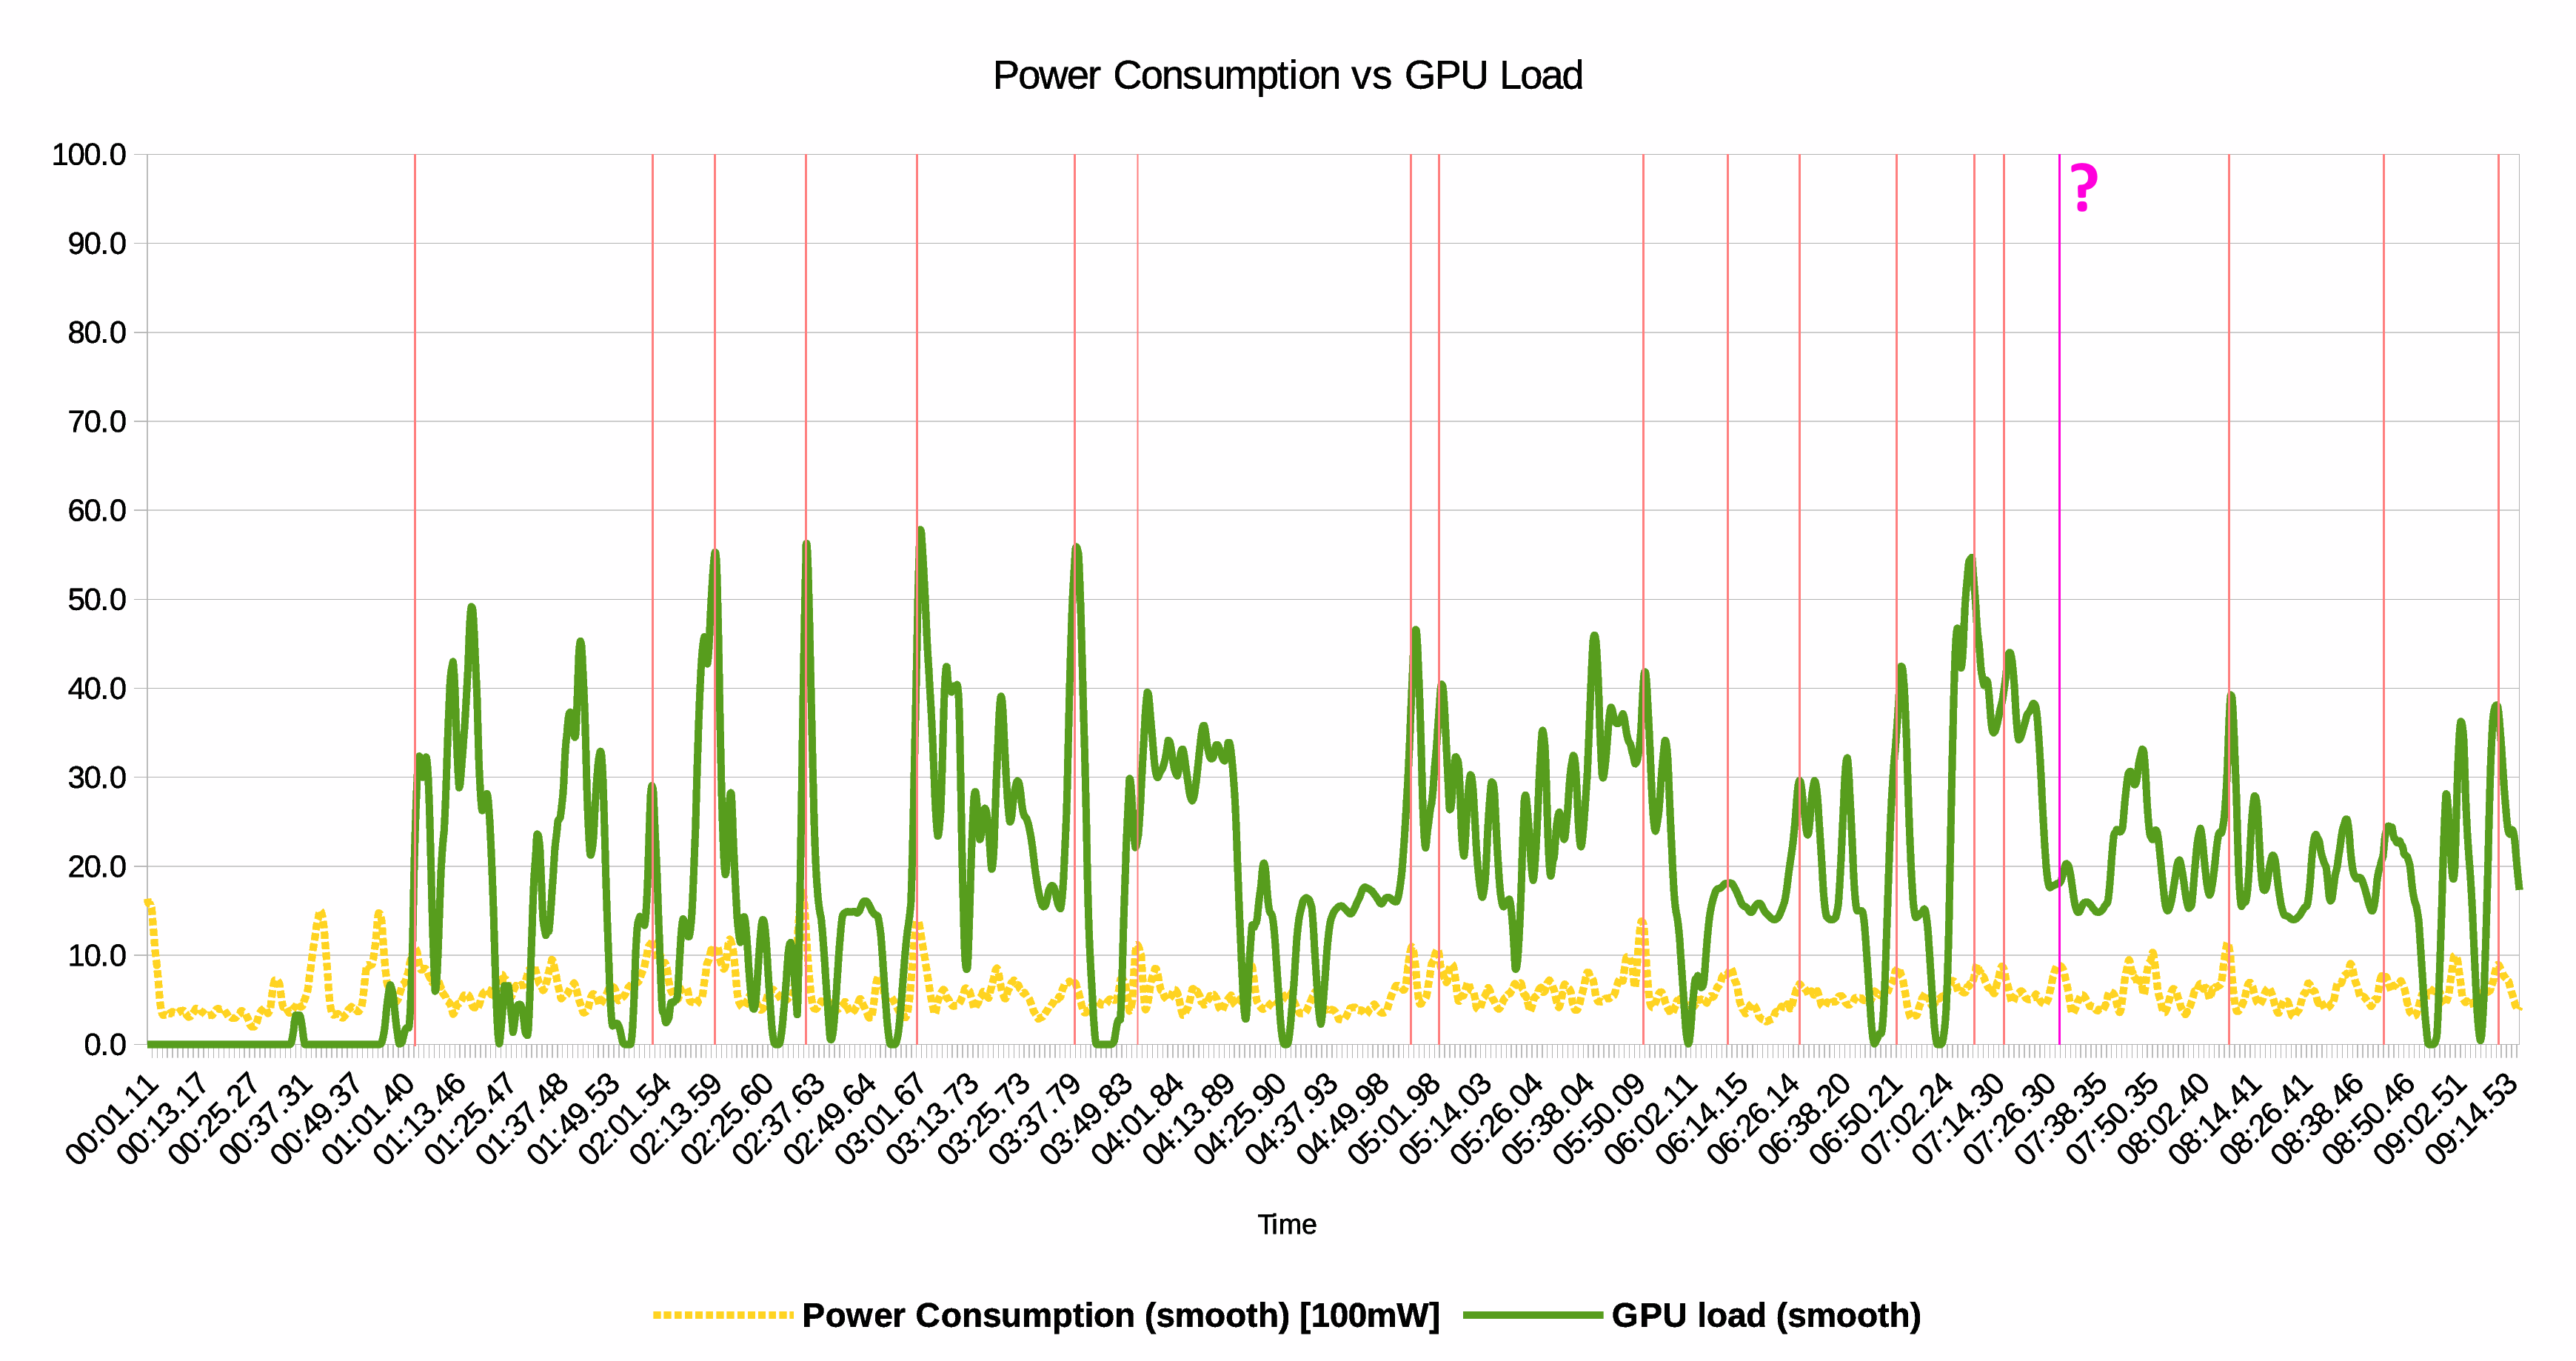
\includegraphics[keepaspectratio, width=0.95\columnwidth]{graphics/GRIT/Measure2D_Power_GPU}\label{fig:power:GPU_2D_contrast:GRIT}}
	 	\end{minipage}
	\caption{Diagram of power measurements with respect to the GPU load, comparing Open Water Levels and GRIT in 2D mode. The less saturated lines show good peak correlations between GPU load and power consumption; the tagged, fully saturated line shows a missing peak correlation. Compared to fig. \ref{fig:power:CPU_2D_contrast}, the majority of missing peak correlations from the CPU band are explained by increased GPU utilisation.}
	\label{fig:power:GPU_2D_contrast}
\end{center}
\end{figure}
%[IMAGES power vs GPU]

%\begin{itemize}
%\item in the first test, we compare the power consumption in relation to \gls{CPU}- and \gls{GPU} utilisation
%\item our initial expectation is the a higher \gls{GPU} load results in an increased power consumption compared to \gls{CPU}-dominated operations, because mobile \glspl{GPU} draw more power than \glspl{CPU} to realise the increased graphics performance
%\item the results are shown for GRIT during 6.5 minutes of operations in fig. \ref{} (split in \gls{GPU} and \gls{CPU} contribution) and for OpenWaterLevel during 3.5 minutes of operations in fig. \ref{}
%\end{itemize}

In both apps, a clear dependency with \gls{CPU} load and power consumption is observable. We can therefore conclude that the mobile processors adapt their clock frequency when less operations are performed, which leads to a reduced power consumption. When comparing \gls{CPU}-related and \gls{GPU} related states, we conclude that while the \gls{CPU} drives the average power consumption, the GPU (being used for rendering images and annotations within them) drives the peak power consumption.

\Gls{GRIT} has two distinct sets of operations, each dominated by either 2D- or 3D tasks, which makes a difference in the ratio of \gls{CPU} load to \gls{GPU} load. The 2D operation mode includes tasks such as photo acquisition and the image-based photo interpretation, whereas the 3D operations include the image-to-geometry registration \cite{Kehl2017_VGC} and the 3D outcrop viewing. Previous figures \ref{fig:power:CPU_2D_contrast:GRIT} and \ref{fig:power:GPU_2D_contrast:GRIT} depict the 2D-dominated cases, whereas fig. \ref{fig:power:CPU_GPU_3D} shows the power consumption relationships in 3D-dominated cases.

\begin{figure}[htbp!]
\begin{center}
	 	\begin{minipage}{\columnwidth}
	 		\centering
			\subfigure[Power to CPU]
			{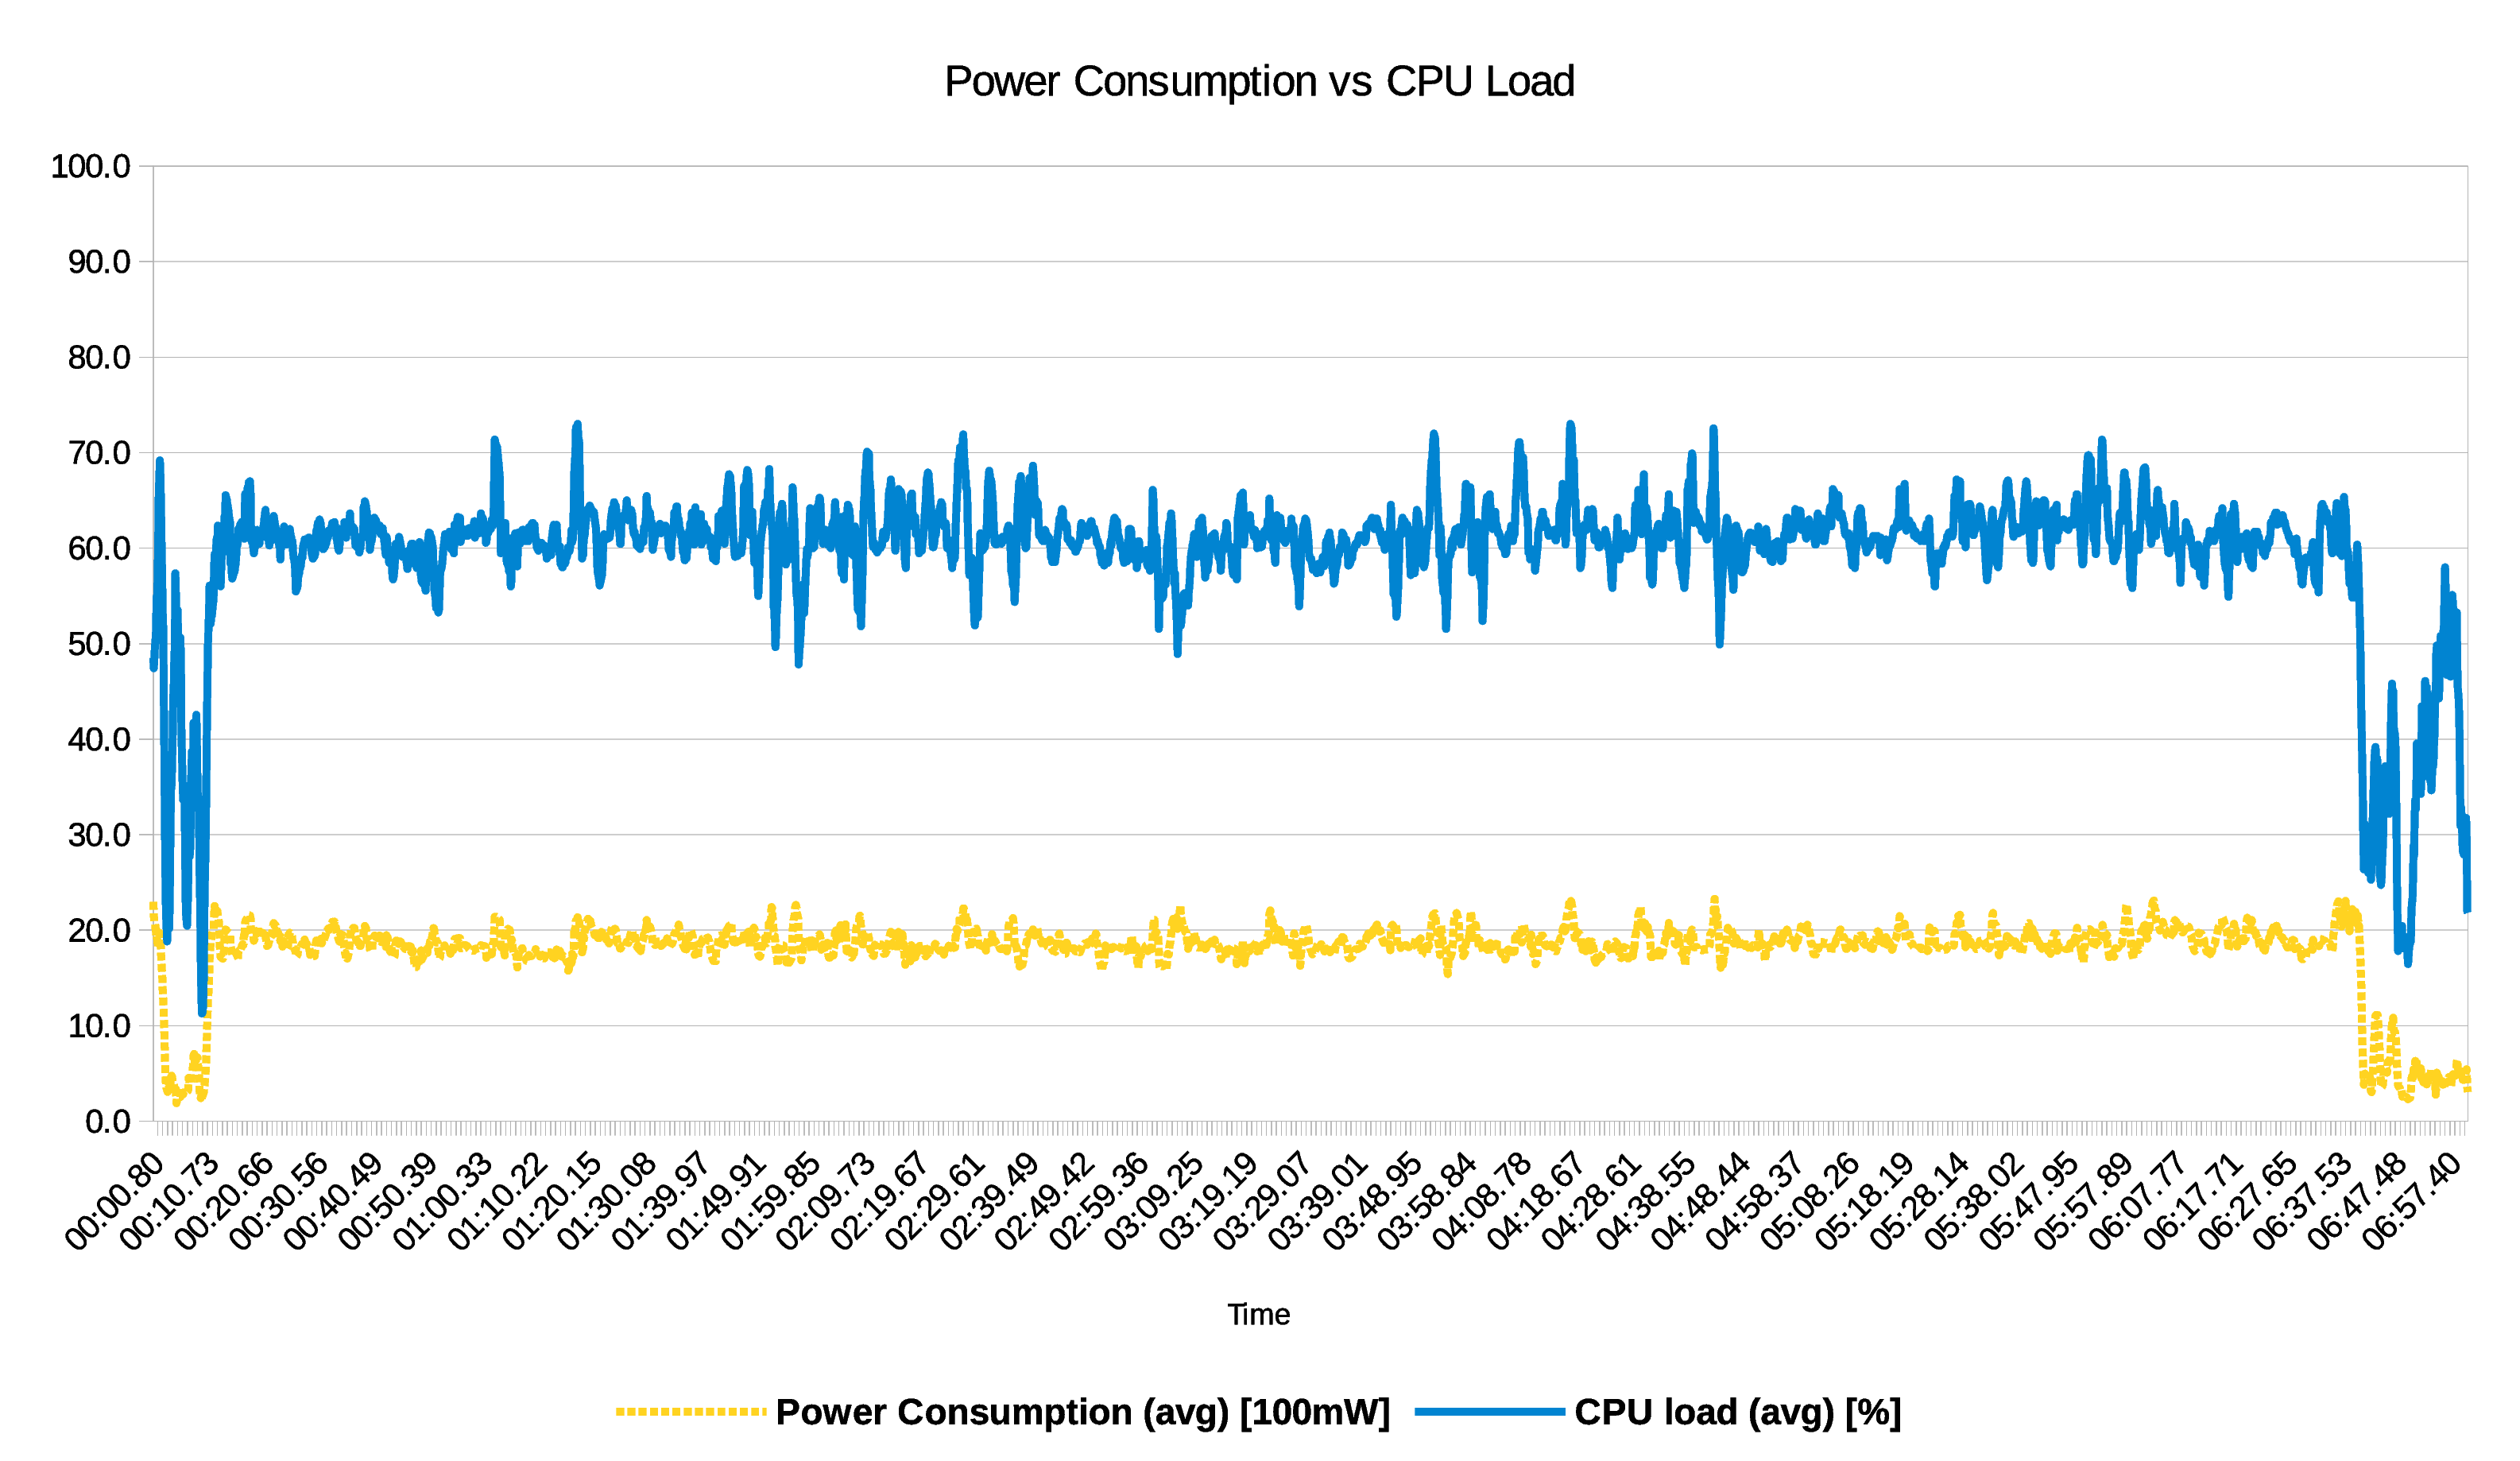
\includegraphics[keepaspectratio, width=0.95\columnwidth]{graphics/GRIT/Measure3D_Power_CPU}\label{fig:power:CPU_GPU_3D:OWL}}
	 	\end{minipage}
	 	\begin{minipage}{\columnwidth}
	 		\centering
			\subfigure[Power to GPU]
			{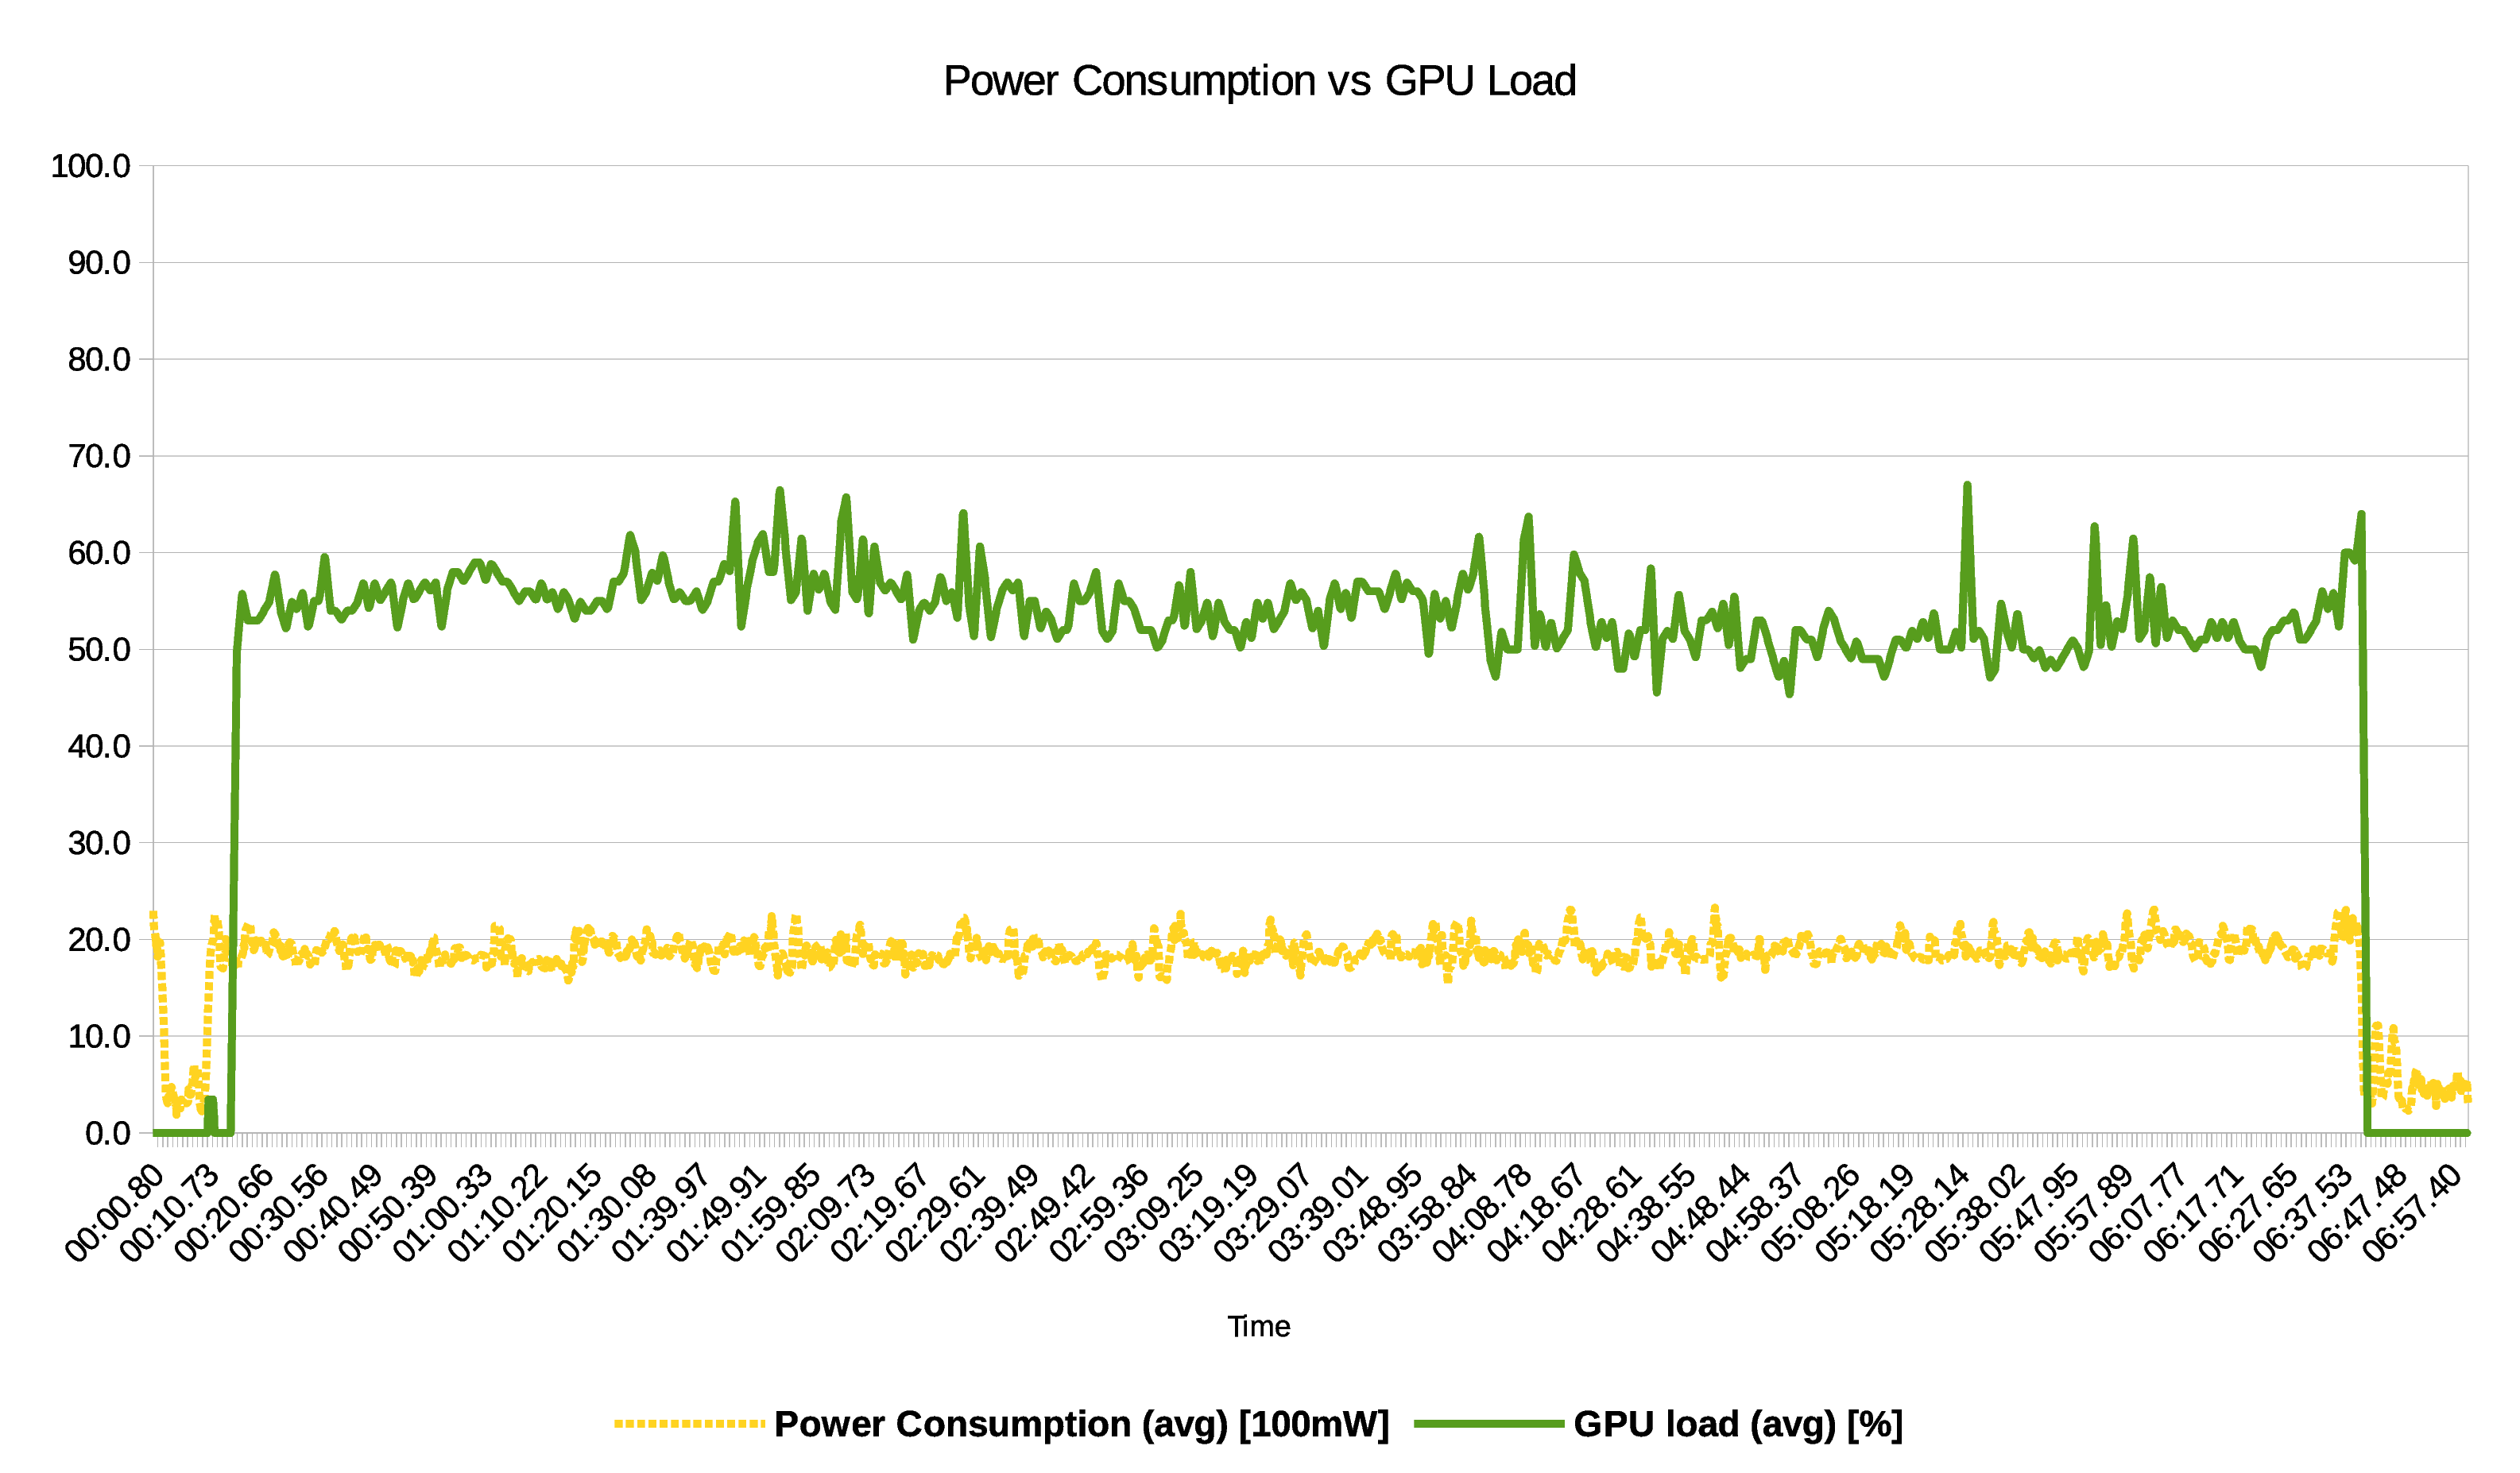
\includegraphics[keepaspectratio, width=0.95\columnwidth]{graphics/GRIT/Measure3D_Power_GPU}\label{fig:power:CPU_GPU_3D:GRIT}}
	 	\end{minipage}
	\caption{Diagram of power measurements with respect to the CPU- \& GPU load of GRIT in 3D mode.}
	\label{fig:power:CPU_GPU_3D}
\end{center}
\end{figure}
%[IMAGES power vs CPU \& power vs GPU in 3D]


\begin{figure}[htbp!]
\begin{center}
	 	{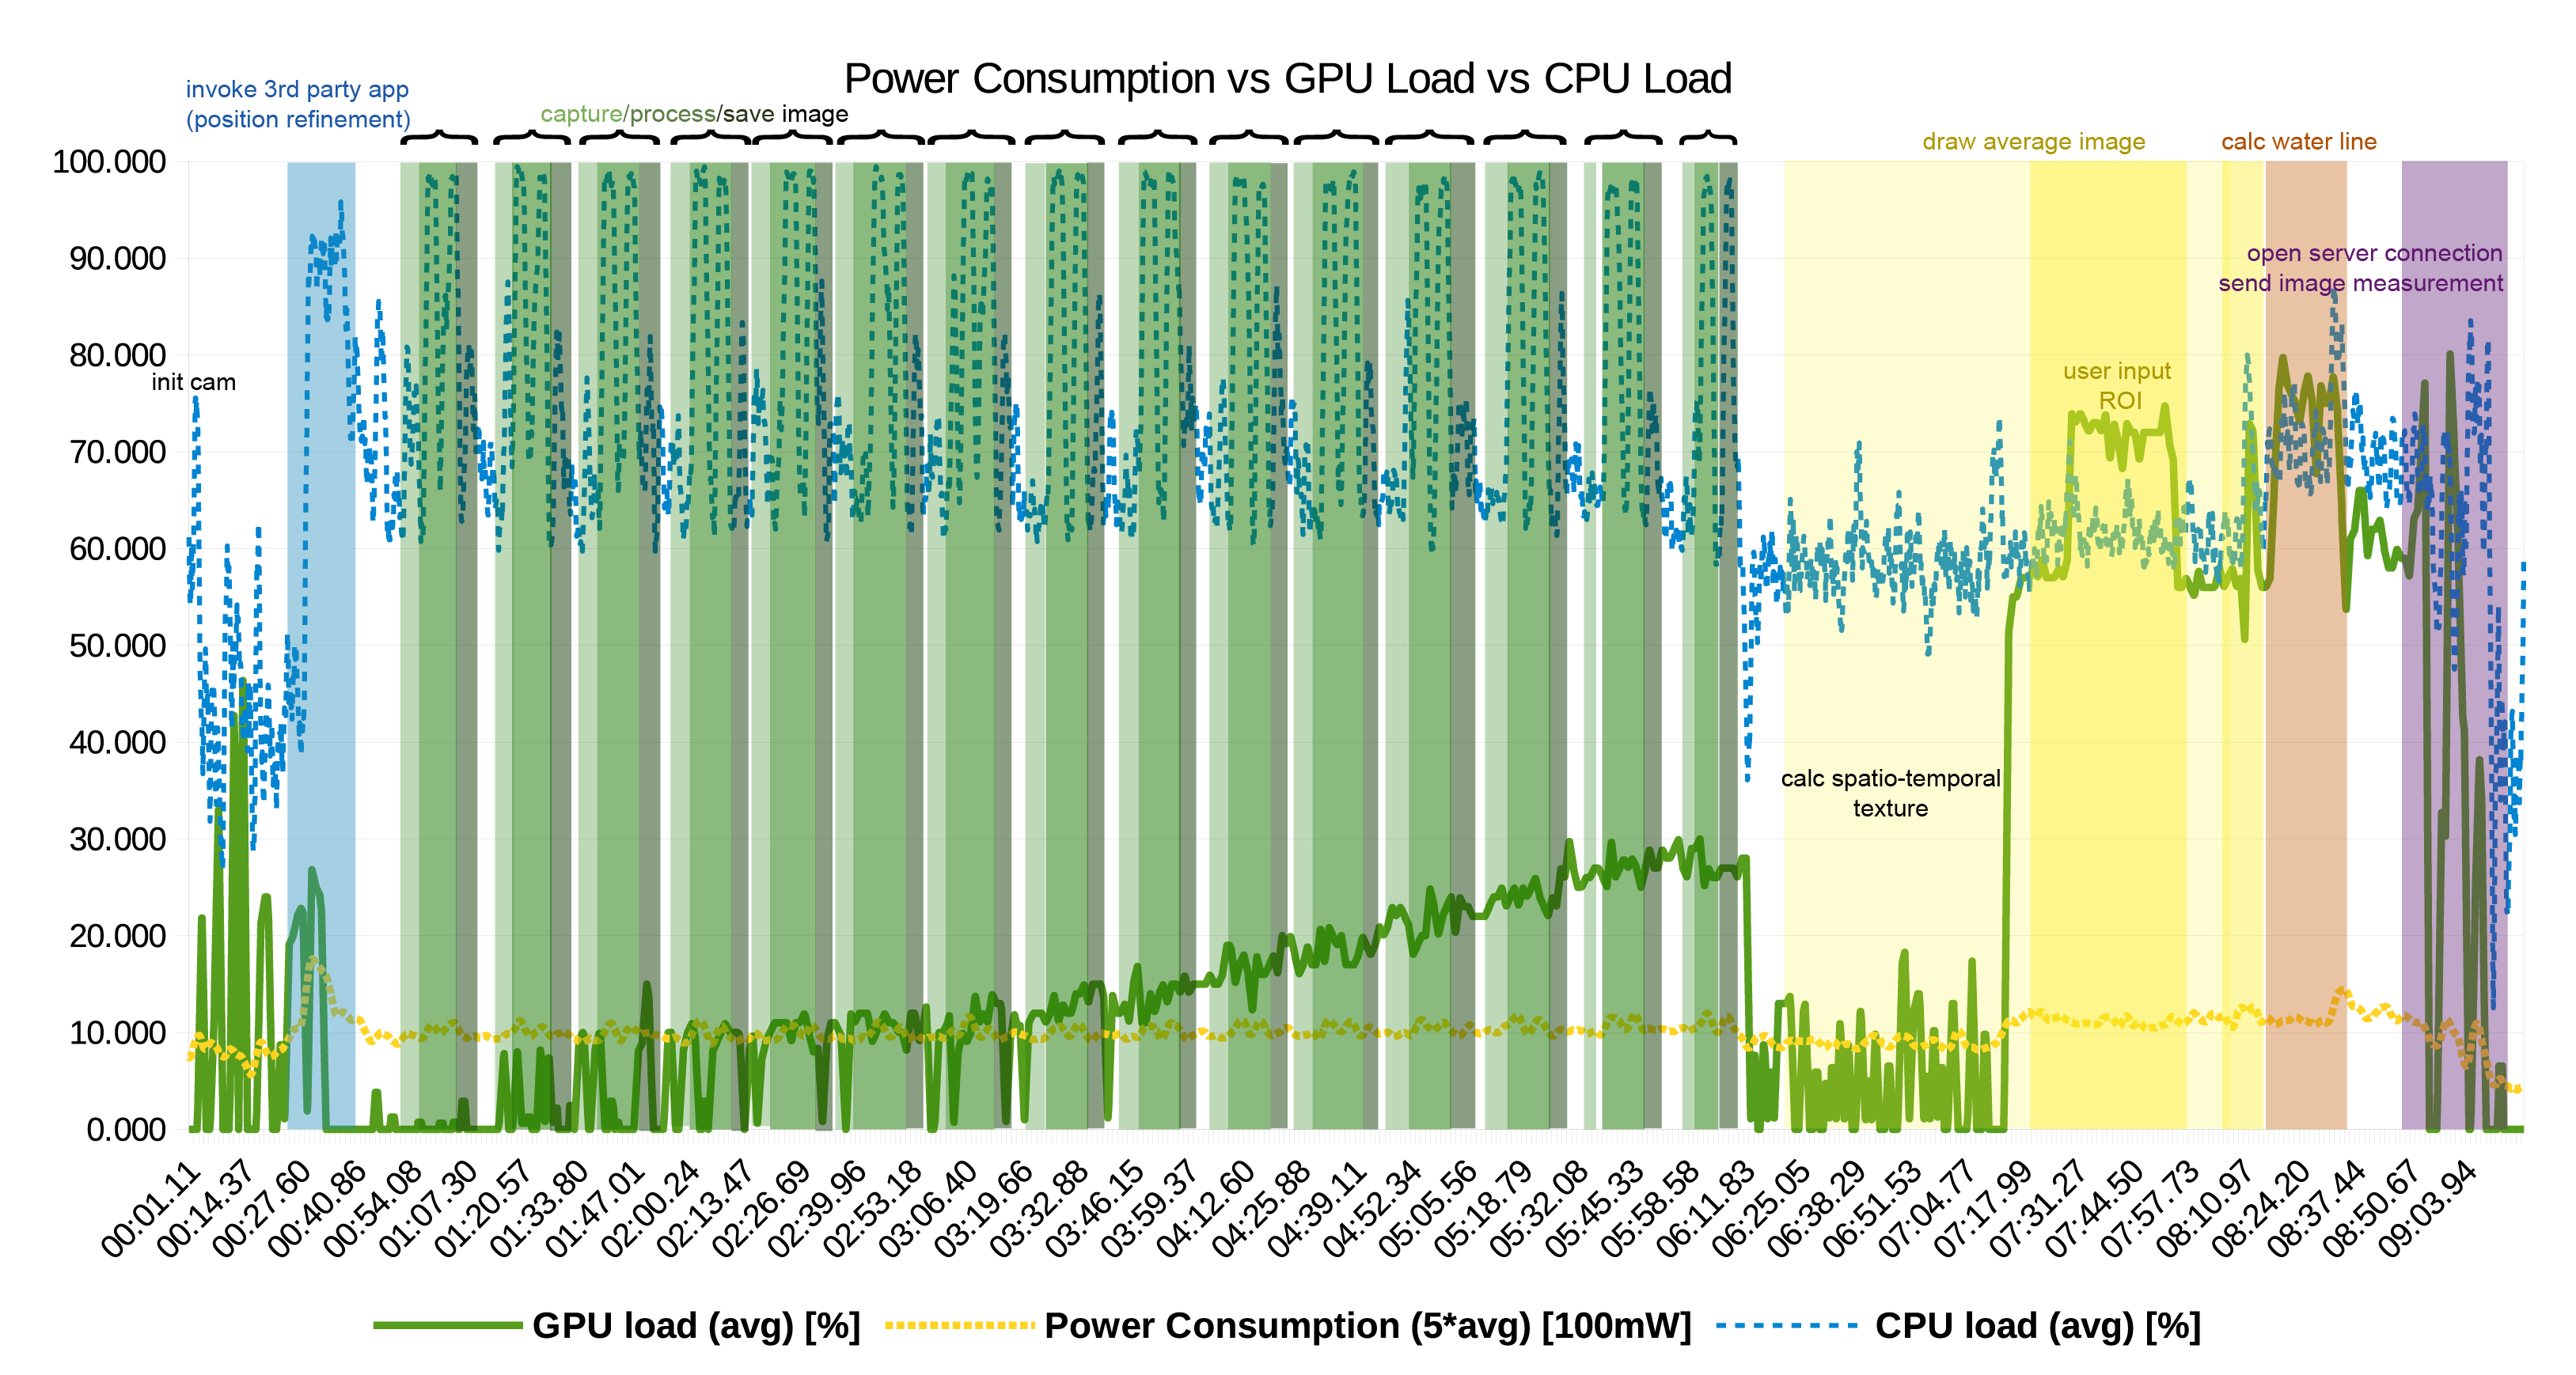
\includegraphics[keepaspectratio, width=0.95\columnwidth]{graphics/OWL_Nexus5/Power_GPU_CPU_run2}}
	\caption{Integrated diagram of power consumption, CPU- \& GPU load of Open Water Levels in 2D mode.}
\end{center}
\label{fig:power:Power_CPU_GPU_OWL:2D}
\end{figure}
%[IMAGES power vs CPU vs GPU in 2D for OWL]


\begin{figure}[htbp!]
\begin{center}
	 	\begin{minipage}{\columnwidth}
	 		\centering
			\subfigure[2D mode]
			{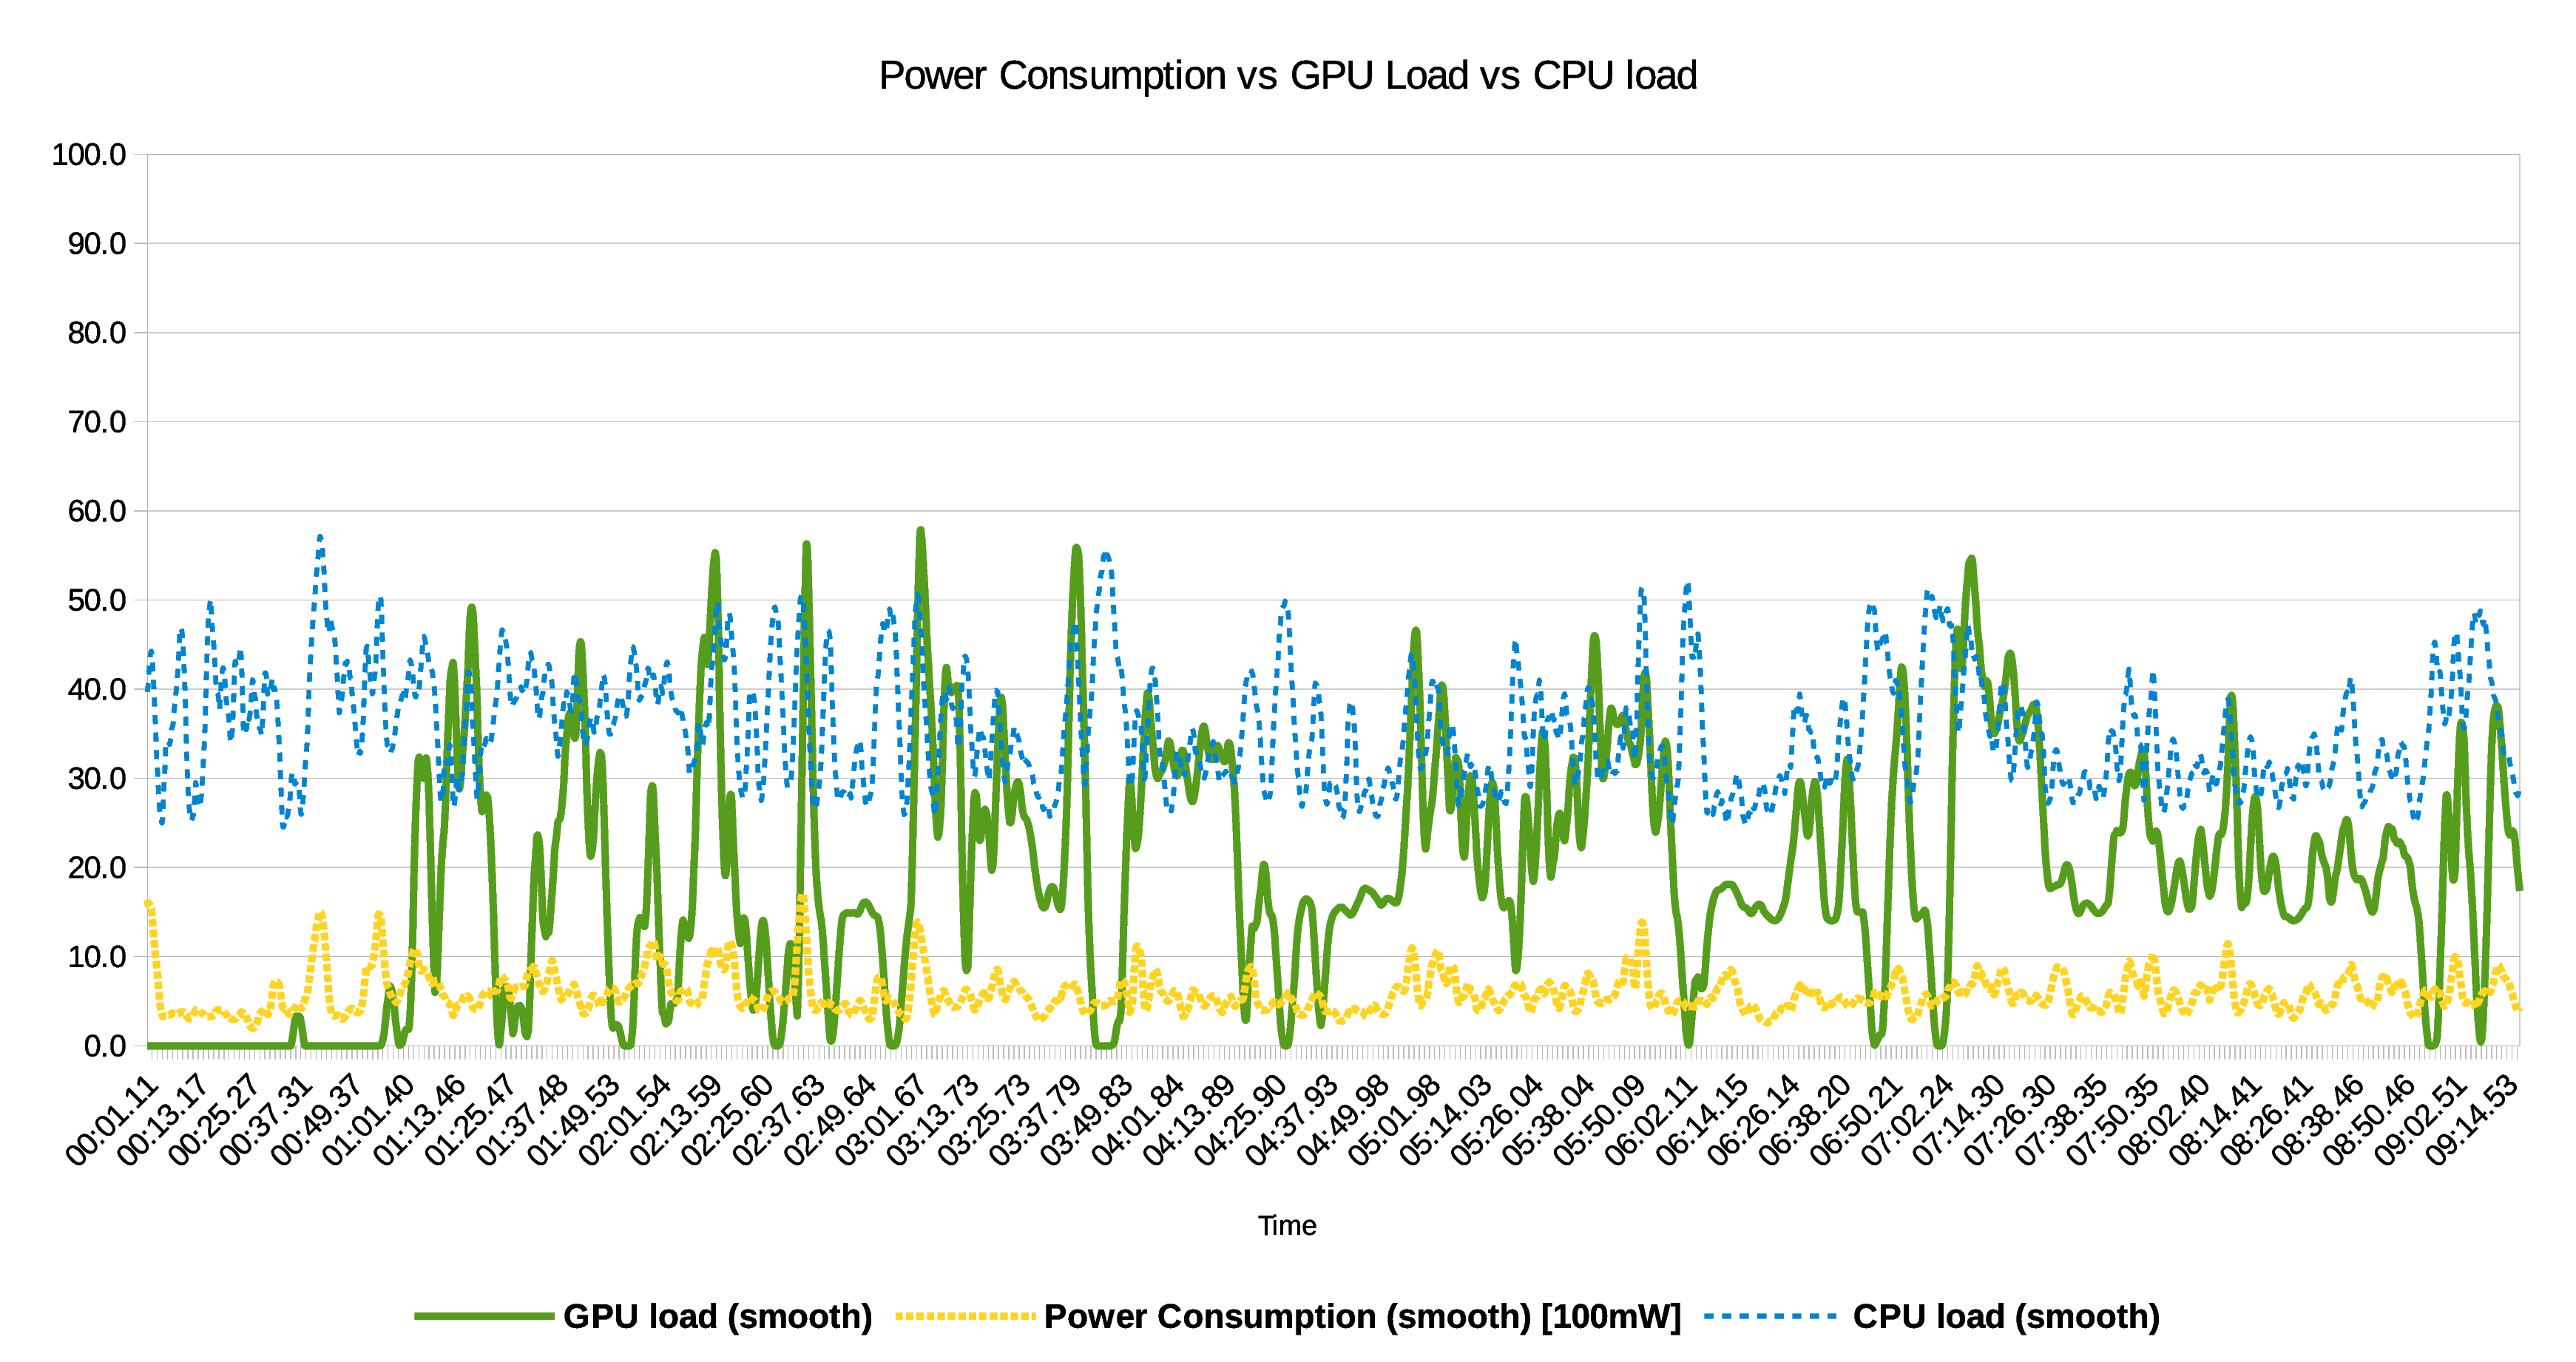
\includegraphics[keepaspectratio, width=0.95\columnwidth]{graphics/GRIT/Measure2D_Power_CPU_GPU}\label{fig:power:Power_CPU_GPU:2D}}
	 	\end{minipage}
	 	\begin{minipage}{\columnwidth}
	 		\centering
			\subfigure[3D mode]
			{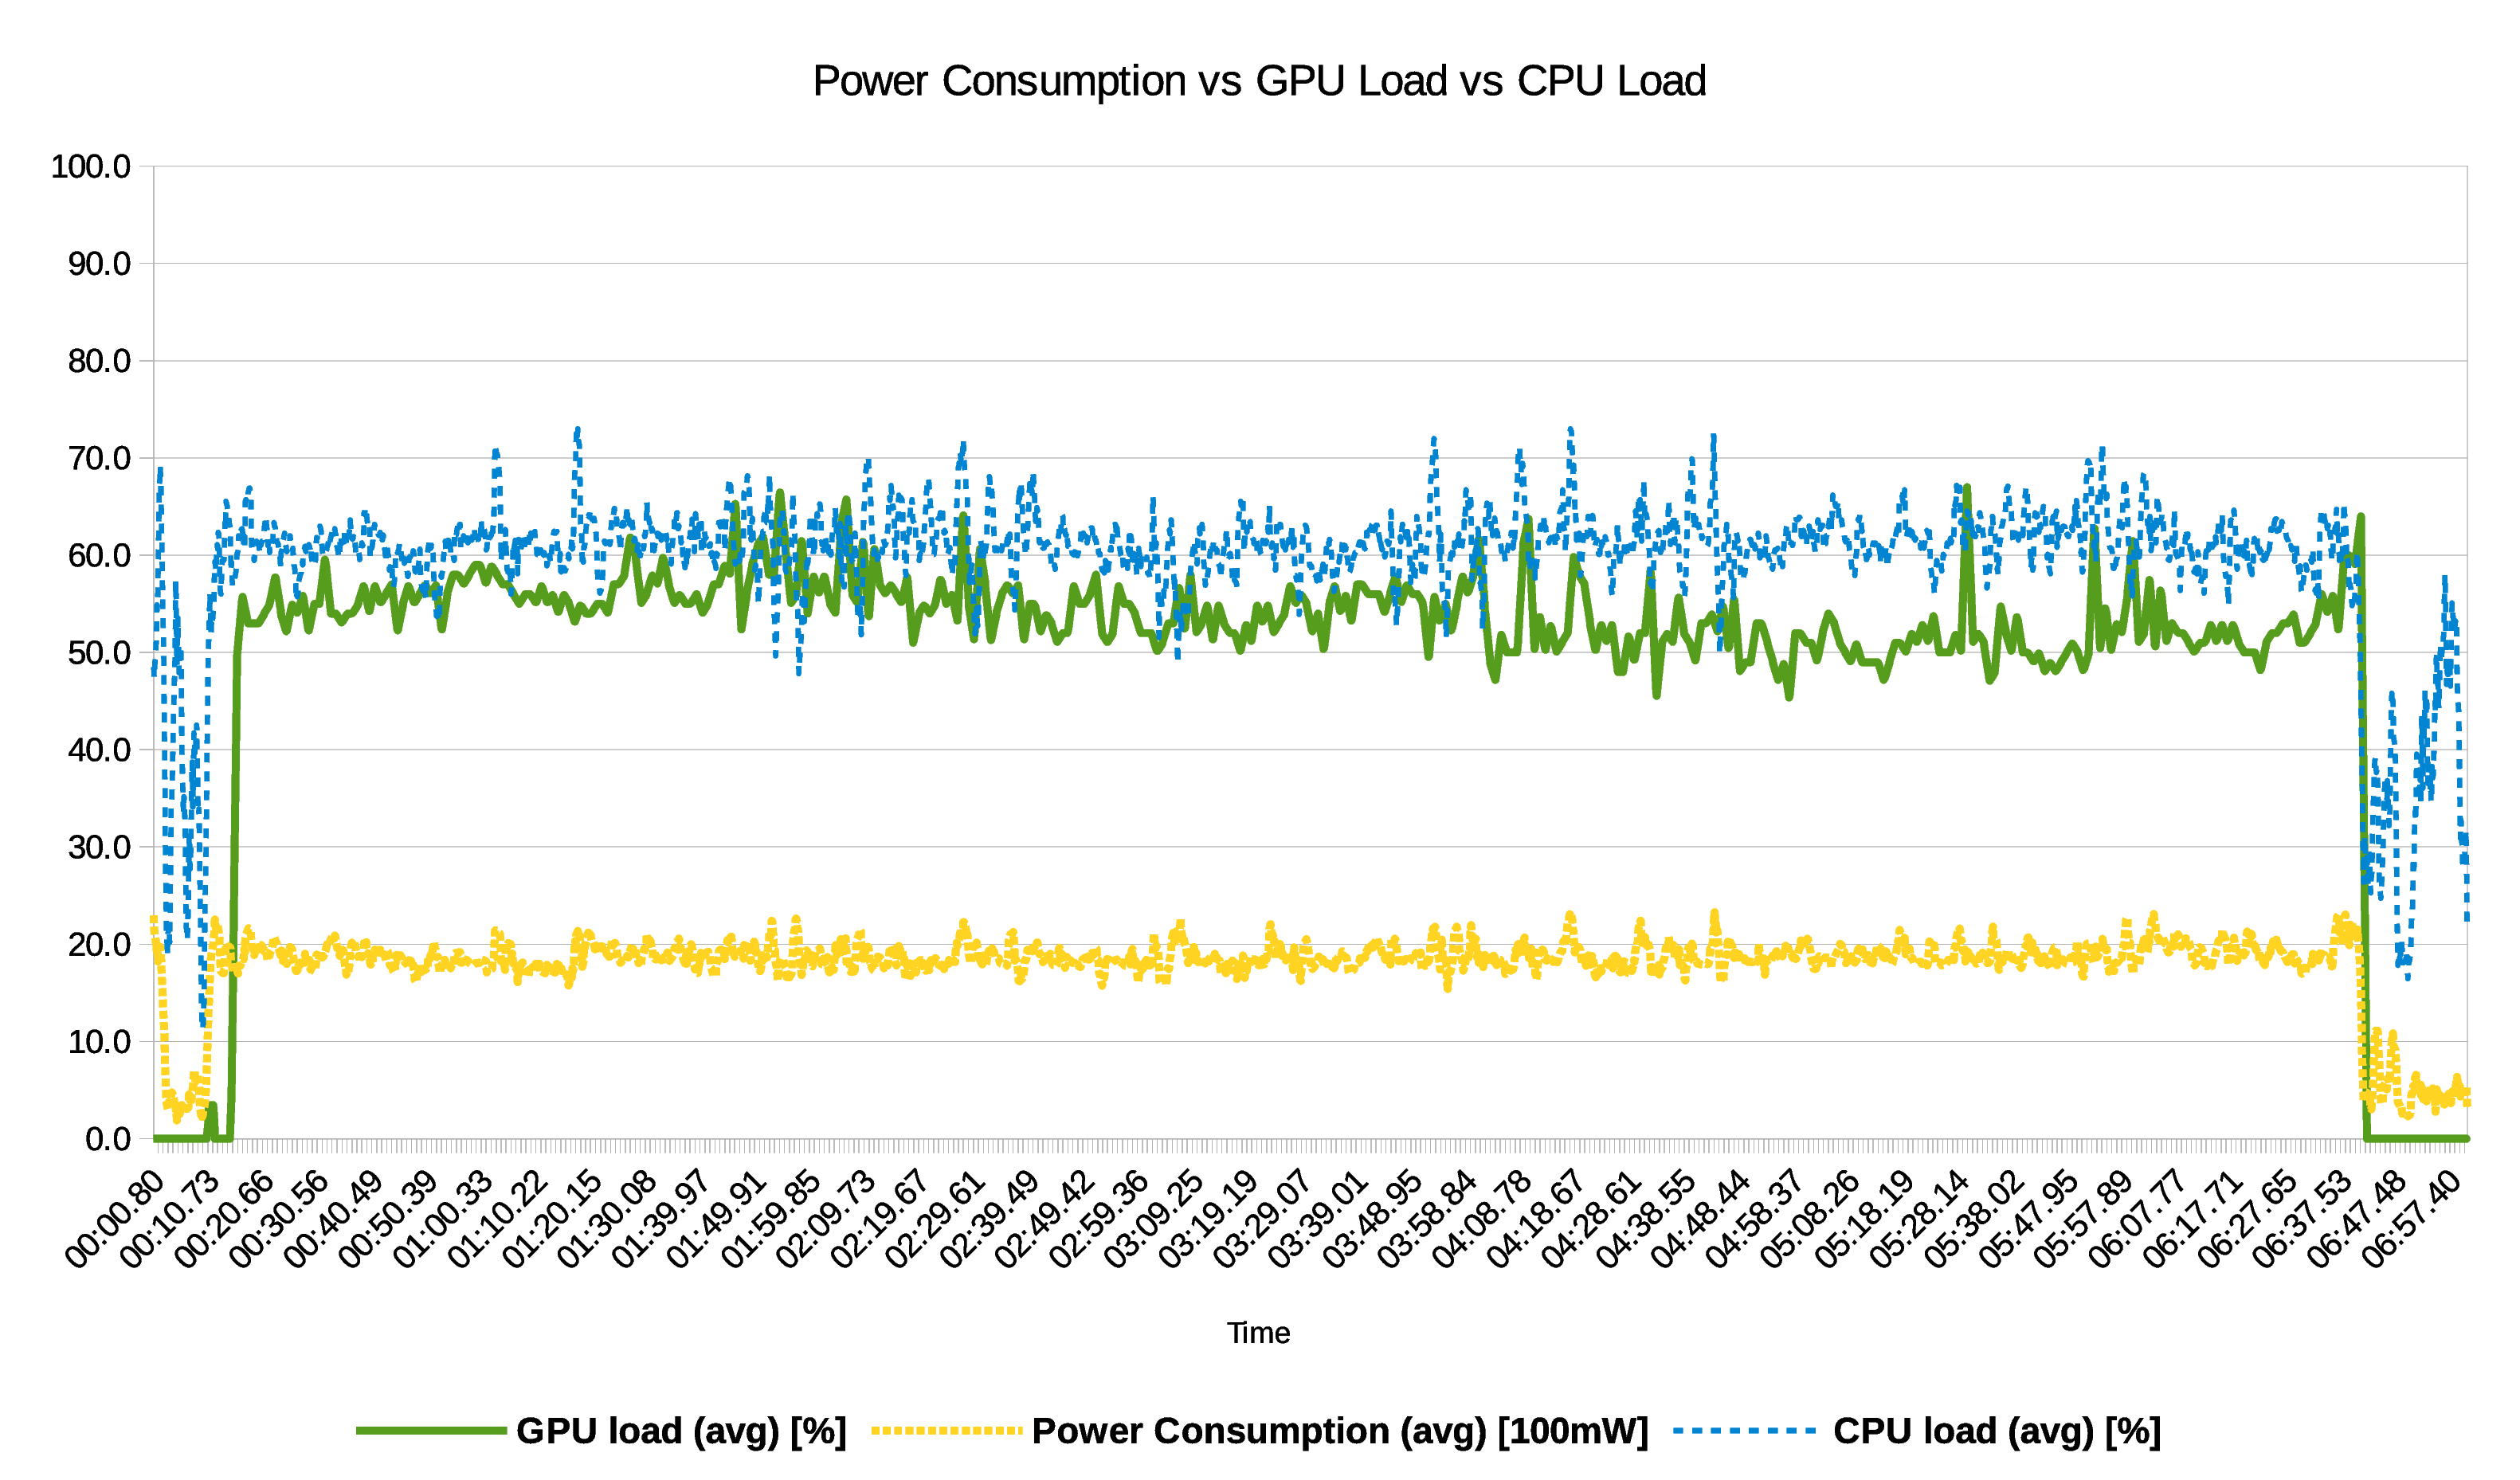
\includegraphics[keepaspectratio, width=0.95\columnwidth]{graphics/GRIT/Measure3D_Power_CPU_GPU}\label{fig:power:Power_CPU_GPU:3D}}
	 	\end{minipage}
	\caption{Integrated diagram of power consumption, CPU- \& GPU load of GRIT in 2D- \& 3D mode. Particular operations, such as image rendering and interpretation editing, are interpreted within the bands as they reult in a distinct \gls{CPU}--\gls{GPU} behaviour.}
	\label{fig:power:Power_CPU_GPU}
\end{center}
\end{figure}
%[COMPARISON IMAGES power vs CPU vs GPU in 2D and 3D]

%\begin{itemize}
%\item observable in both apps: a clear dependency with \gls{CPU} load and power consumption; shows that apps enter a state of conservative energy consumption if being inactive
%\item furthermore, when comparing \gls{CPU}-dependent and \gls{GPU}-dependent energy graphs, we observe that peak energy consumption strongly relates to \gls{GPU} activity
%\item for measurements in ''\gls{GRIT}'', we also have to distinguish between two operation modes
%\item actions such as image-to-geometry registration \cite{} and 3D outcrop viewing employ 3D data processing and \gls{GPU} computations in a major scale, while the image-based interpretation of an outcrop uses 2D image operations within Android-optimized data structures
%\item fig. \ref{} and \ref{} depict the 2D use case, whereas fig. \ref{} and \ref{} show the energy consumption in 3D operations
%\end{itemize}

As clearly observable in fig. \ref{fig:power:Power_CPU_GPU:2D} in comparison to fig. \ref{fig:power:Power_CPU_GPU:3D}, the 3D operations result in a drastic energy cost, raising the average power consumption by around 1220.21 mW. In contrast to novice expectation, the \gls{CPU} load also increases in a 3D data processing setting because the main processors deliver the geometric- and texture data to the \gls{GPU}. Additionally, for the Google Nexus 5 smartphone, the \gls{CPU} needs to decompress the texture image files, resulting in a higher processing load.

Figure \ref{fig:power:Power_CPU_GPU_OWL:2D} visualises the relationship of power consumption, \gls{CPU}, as well as \gls{GPU} for 2D data processing in Open Water Levels. For water line detection, a spatio-temporal texture must be calculated using time lapse images. Thus, the CPU load locally exceeds and falls significantly for each single frame processing (here 15 peaks for 15 images). Unlike \gls{CPU} behaviour, \gls{GPU} load is steadily increasing while storing each co-registered image. After image processing, both \gls{CPU} as well as \gls{GPU} load are released whereas app modifications via user interface leads, as expected, once more to higher loads.

%\begin{itemize}
%\item as clearly observable in fig. \ref{} in comparison to fig. \ref{}, the 3D operations result in a drastic energy cost, raising the average power consumption by XYZ mW
%\item in contrast to novice expectation, the \gls{CPU} load also increases in a 3D data processing setting
%\item that is because the \gls{CPU} of the mobile processor needs to deliver the geometric- and texture data to the \gls{GPU}; also, the \gls{CPU} needs to decompress the texture image files, resulting in a higher processing load
%\end{itemize}

The conclusions of this power consumption study for field apps is manifold. We obtained benchmark measurements for specific target apps in hydrology (Open Water Levels) and geology (\gls{GRIT}), and explained how to replicate the study on Android devices with other field apps in the future. For Open Water Levels, the app can be operated on an average of of 1090.41 milliampere per hour (natively measured in milliampere), allowing a theoretical operability of 2.11 hours on the Google Nexus 5. For \gls{GRIT}, we have to distinguish between the mode in which it is operated: when conducting 2D operations, the app consumes 568.50 milliwatt per hour, which results in an operation time of 14.56 hours at an average current of 3.6V. When making full use of the 3D capabilities of \gls{GRIT} all the time, the average power consumption rises to 1788.80 milliwatt per hour, which results in an operation time of only 4.63 hours at an average current of 3.6V. The applied current for the GRIT measurements is of theoretical nature, applied because the measurements were taken in watt exclusively while the battery capacity of mobile devices is commonly given in milliampere hours (mAh). Furthermore, we highlight these measurements as being the \textit{theoretical} operation time because most users have other apps and background services open on their mobile device that simultaneously consume power, further reducing the operation time. Lastly, as stated by Carroll et al. \cite{Carroll2010}, the app-specific consumption (in particular with ''visual apps`` and the sensor applications) also depends on the screen brightness and the sensor usage. Key measures on power consumption, and related metrics of processor temperature and memory usage, are given in table \ref{table:power:GRIT} for \gls{GRIT} and table \ref{table:power:OWL} for Open Water Levels.

\begin{center}
\begin{longtable}[HT]{| l | p{2.5cm} | p{2.5cm} |}
	\caption{Average measurements of GRIT}
	\label{table:power:GRIT}
	\endhead
%\begin{center}
	%\centering
	%\begin{tabular}{| l | p{1.8cm} | p{1.8cm} | p{1.8cm} | p{1.8cm} | p{1.8cm} | p{1.8cm} | p{1.8cm} | p{1.8cm} | p{1.8cm} | p{1.8cm} | p{1.8cm} | p{1.8cm} |}
		\hline
		metric & 2D ops. & 3D ops. \\ \hline
		power consumption [mW/h] & 568.59 & 1788.80 \\ \hline
		power consumption [mA/h \@ 3.6V] & 157.94 & 496.89 \\ \hline
		memory usage (avg.) [GB] & 1.746 & 1.721 \\ \hline
		temperature [$^{\circ}$C] & 49.91 & 52.05 \\ \hline
\end{longtable}
\end{center}

\begin{center}
\begin{longtable}[HT]{| l | p{2.5cm} | p{2.5cm} |}
	\caption{Average measurements of Open Water Levels}
	\label{table:power:OWL}
	\endhead
%\begin{center}
	%\centering
	%\begin{tabular}{| l | p{1.8cm} | p{1.8cm} | p{1.8cm} | p{1.8cm} | p{1.8cm} | p{1.8cm} | p{1.8cm} | p{1.8cm} | p{1.8cm} | p{1.8cm} | p{1.8cm} | p{1.8cm} |}
		\hline
		metric & Google Nexus 5 & Samsung S8 \\ \hline
		power consumption [mA/h] & 1090.41 & ? \\ \hline
		memory usage (avg.) [GB] & 1.543 & ? \\ \hline
		temperature [$^{\circ}$C] & 58.55 & ? \\ \hline
\end{longtable}
\end{center}

In more general terms applicable to the geoscience domain, the study shows that users need to be aware of what data they are dealing with in order to get the maximum operation time and most efficient workload done during the field study. This will have implications for fieldwork planning for expert users and practitioners, as they can modify their study plan to first collect photos, observations and interpretations from several viewpoints of their study objective and then use 3D operation features ''in burst`` for visual checks and data interrogation before moving on to subsequent study locations. Insufficient planning and an overuse of 3D field app features can reduce the effective ''digital fieldwork`` time using \gls{GRIT} to 9.26 hours at best when carrying one external battery pack. Also, with this measure we want to highlight that the operation time error in the measurements is significant because we need to assume an average current of 3.6V, which may be far off when comparing the measurements to \textit{Open Water Level}. Considering the \gls{CPU} load behaviour in 3D-mode of \gls{GRIT}, we can also hypothesize about the positive impact of utilising hardware-specific operations, such as \gls{GPU} texture decompression, on the energy consumption: while using the \gls{GPU} requires generally more power, it is also more efficient in operations such as texture decompression, therefore potentially having a positive affect on the overall power consumption of 3D mobile field apps.

%\begin{itemize}
%\item conclusions from the measurements are manifold
%\item on the level of assessing the profiled apps ''OpenWaterLevel'' for hydrological studies and ''\gls{GRIT}'' for field geology studies, we obtained benchmark measures for their power consumption
%\item for OpenWaterLevels, the app can be operated with an average of 1090.41 mA per hour (measured as mA/h), allowing a theoretical operability on a Google Nexus 5 smartphone of 2.11 hours
%\item for \gls{GRIT}, we distinguish between 2D- and 3D operability
%\item in 2D operation mode, only conducting image-based interpretations, \gls{GRIT} consumes 568.59 mW per hour, allows around 14.56 hours of operation at 3.6V (if this app would be the only app running)
%\item on the other hand, if being operated consistently in 3D-mode, the same app consumes 1788.80 mW per hours, allows only 4.63 hours of (exclusive) operation at 3.6V
%\item more generally speaking, the study shows that it is important for geoscience users to be aware of the which data they are working with on the mobile device
%\item even though 3D may be readily available for a given study, it is not advisable to access them on the mobile device over stretched periods, as the drastically increased power consumption results in an operation time of XYZ hours with two external power packs in the field bag
%\item considering the \gls{CPU} load behaviour in 3D-mode, we can also hypothesize about the positive impact of utilising hardware-specific operations such as \gls{GPU} texture decompression on energy consumption: while using the \gls{GPU} requires generally more power, it is also more efficient in operations such as texture decompression, therefore potentially having a positive affect on the overall power consumption of mobile field apps
%\end{itemize}

\section{Applications and Requirements}
\label{sec:applications}
Due to the increasing usability of mobile devices for in the field annotations, several use cases concerning geosciences has become apparent. In the following, two \textcolor{blue}{Chris: or three} key applications are subsequently presented: water level gauging through field observations for small and medium-sized catchments, geological interpretation of sedimentary features in field geology, and the use of mobile devices in virtual field trips.

\subsection{Derivation of hydrological parameters: Water level gauging}
\label{sec:water_level_gauging_intro}
The past decade is characterized by a continued increase of globally devastating flash floods after heavy rainfalls. Even smallest creeks turned into hazardous streams causing flooding and landslides. Conventional gauging stations provide precise information about water levels measured over a short time period. State of the art techniques for administrative observation comprise of water pressure sensors, floating gauges and conventional tide gauges. They are characterised by long-term stability and outdoor robustness providing accuracies of several millimetres up to one centimetre \cite{Siedschlag2015}. Averaged over defined time intervals, it is advisable to remain cautious regarding these accuracies possibly being too optimistic \cite{Horner2018} . 
 
Because of high costs in purchase and maintenance, gauging stations with complex sensing devices are sparsely installed. A prime example here is the hydrological network in Saxony, Germany. There, 184 gauging stations are installed for permanent observation on 154 of 259 rivers rising from small, medium and large catchments \cite{Saxon2018, Buettner2015}. Thus, around a third is not monitored neither during flood events when the most protection is required. Recently, commercial smartphone applications arose to enable crowd-sourcing based water level estimation (see \cite{CrowdWaterApp2017a,Kisters2014} for details). All of them have one thing in common: the water level is entered manually by engaged citizen scientists finding and photographing tide gauges close to rivers that presents, on the one hand, a potential danger to themselves (f.e. by sudden landslides), and still limits on the other the approaches to open and visible gauges.

Improvements in this sense can be achieved through image-to-geometry intersection and 3D annotation for automatic water level determination without reference gauges for almost every situation regarding running waters. 
For this, the smartphone application \textit{Open Water Level} is developed, which is based on the freely available open source camera framework \textit{Open Camera} \cite{Harman2017}. Open Water Level allows for free stationing water line detection using short, handheld time-lapse image sequences \cite{Kroehnert2017a}. To interpret these, image measurements must be transformed into object space. Thus, exterior information needs to be provided by smartphone sensors for orientation and positioning.

\subsubsection{Requirements applying to the sensors}
\label{sec:water_level_gauging_requirements_sensors}
To solve the task of autonomous water level determination on running rivers via image-to-geometry intersection, the citizen scientist's position and orientation must be know. As figured out in \ref{sec:technology}, smartphone sensors accuracies for orientation and location are highly dependent on user's environment. Especially the strong correlation of heading and disturbing magnetic sources may be a issue must be solved specifically related to running rivers where metal railings usually exists. Similar effects can also be noted using high-end IMU systems, for instance autonomous car navigation. In contrast to outdoor measurements, the magnetic influences inside cars are almost stable and can be pre-calibrated (advanced navigation manual). For smartphone orientation, the magnetic strengths attaching the phone may change substantially in short time. A typical scenario would be: a citizen scientist walks along street, taking his phone inside the baggage close to metallic keys. While walking he passes several street lamps, signs, etc. Finally, he arrives at a bridge over a urban river, takes out the phone, looks down to the river and records the time lapse image sequence a few centimetres above a metallic railing. Meanwhile, several cars passing the same bridge. In this simple use case, the magnetic field around the smartphone changes countless times due to several unpredictable disturbances \textcolor{red}{(table_mag_disturb)} \cite{Blum2013}.

The heading angle has the highest influence compared to pitch and roll regarding 2D image and 3D object data registration. For this, a so-called synthetic image is rendered from coloured 3D reference point clouds using the scientist's location and orientation to define a situation-dependent bounding box of points to be projected onto image plane with respect to depth and indentations (see \cite{Boerner2016}). Thereby the heading defines the rotation of the depth direction, as a false angle gives a false viewing direction resulting in a synthetic image that has little--to--no similarity with the time lapse sequence. However, in case of no similarity and thus no possible solution for image-to-geometry intersection, the water level calculation simply fails. In case of slight overlapping, there might be image matches but with insufficient point distribution that impedes a correct positioning \textcolor{red}{(fig_heading_test)} and may lead to even worse results of false water levels.

The absolute geo-positioning of installed \gls{GNSS} receivers on current smartphones is another obvious error source. In urban scenes with several shadow effects due to high-rise buildings, as well as in situations of heavy cloud coverage, errors of several metres in latitude and up to more than 30 metres in altitude are highly possible \cite{Bauer2013, Blum2013, Zandbergen2011}. It is likely that, in the near future, smartphone's \gls{GNSS} modules will be improved, solving lateral accuracies of 50 centimetres \cite{Moore2017}.

For now, possible relief can be provided by other sources for positioning, like digital elevation models for simple height correction or invoke map services that allows the user for position refinement. For this, some APIs are already provided by Google\footnote{Google Maps Geolocation API - \url{https://developers.google.com/maps/documentation/geolocation/intro}}, but they are rather power consuming when accessed continuously. Another upcoming option is including barometers in sensor fusion, where altitude can be measured within three meters \cite{Liu2014}.


\begin{itemize}
\item(table, observation heading during water line detection outside $\rightarrow$ check magnetic strengthens and there changes over short times)
\item (figure/table, sensitivity analysis  $\rightarrow$ heading changed in terms of 10 degrees, what does it make for)
\end{itemize}


\subsubsection{Requirements applying to the scenario}
\label{sec:water_level_gauging_requirements_situation}



\begin{itemize}
\item \textit{online processing and position refinement: need online connection}
\item \textit{image quality for water line detection: influence of image resolution, lightning, ...)}
\end{itemize}





\begin{itemize}
%\item recap: task to be solved
%\item main requirements for (location- and orientation) sensor accuracy and geometric accuracy
%\item specific requirements to this use case: data availability; illumination; device range to cover
\item available approach to address the task
\end{itemize}

\subsection{Field Geology}
\label{sec:applications:field_geology}

The goal of geological fieldtrips is to gather insight in the rock record and the structural- and sedimentary rock architecture of a given location. Rock architecture can be studied within subsurface seismic records, but this approach suffers from inferior imaging resolutions and physical limitations of the surveying technique. Therefore, surface outcrops are used for the study. Outcrops can be scanned with modern equipment (e.g. \gls{LiDAR} \cite{Buckley2008a,Buckley2010}, drones \cite{Dewez2015} and \gls{SfM} \cite{Chandler2016}) to generate digital surface representations. The most common representations of digital outcrops are coloured point clouds and textured \glspl{TIN}.

The geological aspect is introduced by interpreting the outcrop models. In this case, interpretations refer to (i) line marks for separating stratigraphic layers, (ii) surface-projected polygons to highlight structural- and sedimentary facies or specific architectural elements and (iii) minor ticks (e.g. lines, points, patterns) to indicate supplementary attributes such as deposition orientation or grain geometry. The interpretations was, until recently, performed in a two-step process: sketches are drawn by hand in a dedicated fieldbook to document the geologist's observation of the architecture. After the fieldtrip, the observations are digitised in the office by transferring the sketched architecture on the available digital outcrop. From there on, further study goals (e.g. geomodelling) are pursued. As recently published, this workflow is currently being transformed into an integrated digital workflow in the field using mobile devices (see \cite{Kehl2018_AGU} for further details).

Geological interpretations can be documented on various scales, but from observations of the author most interpretations are conducted on medium-range. This results in an average observation distance for architectural interpretations of between $100m$ to $500m$ to document individual depositional elements, and further distances of around $400m$ to $1400m$ to document the overall stratigraphic framework of an outcrop. These distances can vary to some degree depending on the physical accessibility of an outcrop. Therefore, as a result of perspective observations, the required lateral localisation accuracy is in the range of $\leq 2.5m$ for the individual element setting and $\leq 8m$ for the wide-angle stratigraphic setting. While achieving the former resolution can still be challenging with mobile sensors (see section \ref{sec:technology:sensors:localization}), the latter resolution is almost guaranteed for \gls{GPS} localisation. The more important problem is in the vertical resolution: the vertical position has, especially in close-distance observations, a drastic impact on the view perspective. Even more important, a vertical localisation error of  $\geq 1.5m$ may result in positioning the mobile device ''under ground'', making any image-based registration impossible. It is this vertical accuracy that is crucial for mobile device interpretation systems to work. Several improvements, such as \glspl{DEM} and barometric altitude \cite{Kehl2017_VGC}, have been proposed to reduce the vertical positioning error while there is still room for novel research proposals to provide more accurate vertical positioning or ground-based constraints on the altitude estimation.

One of the dominant challenges for digital field geology is the free availability of 3D surface models. Currently, research groups in the domain (e.g. from the University of Manchester \cite{Hodgetts2013}, Durham University \cite{McCaffrey2005}, University of Aberdeen \cite{Howell2014}, University of Bergen and UniResearch CIPR \cite{Dreyer1993}) are building their own digital outcrop databases. Due to the strong industry involvement, these and other databases (see SAFARI \cite{Dreyer1993} and FAKTS \cite{Colombera2012a}) are excluded from public access. Recent developments aim at providing digital outcrops in an open-access manner \cite{Cawood2018} to resolve the issue. Furthermore, due to the vertical positioning problem above, easy access to high- and medium resolution \glspl{DEM} is important. As demonstrated by recent measurement, the usage of \glspl{DEM} has a significant influence on the projection accuracy of image-based interpretation on mobile device towards 3D surface models \cite{Kehl2017_VGC}.

One particular challenge in digital field geology is the treatment of environmental changes. Digital outcrops are infrequently collected and the textured models are used for field study all across the year. Therefore, in image registration terms, there is a drastic difference in local illumination, moisture content as well as fog and snow between acquired 3D surface models and the outcrop images collected during field trips. The issue has been previously discussed in terms of illumination differences \cite{Kehl2017_PHOR}, but drastic changes in terms of fog and moisture are still problematic to treat. Therefore, it is advisable to collect digital outcrop models for prominent locations in different seasonal conditions to allow for variety in model selection when planning field trips.

Currently available systems that provide digital outcrop interpretation capabilities on mobile devices in 3D include \gls{GRIT} \cite{Kehl2016_VGCabstract} and Outcrop \cite{Viseur2014_VGCabstract}, though earlier prototypes have been demonstrated \cite{Hama2013}. Outcrop, developed by \gls{CEREGE} at Aix-Marseille Universit\'{e}, is a mobile device app for Android devices that is able to load and process various forms of numerical outcrops. Its major focus is the documentation of structural features (e.g. fault areas, fractures and rock deformations) on outcrops using line interpretations. Furthmore, it is possible to pin extended note annotations to the model. \gls{GRIT}, developed as a collaboration between UniResearch AS CIPR, University of Bergen, University of Aberdeen and \gls{CEREGE}, is a mobile app for Android devices that can handle large-area digital outcrops of tens of kilometres is surface length in 3D. Its major focus is the documentation of the sedimentary- and stratigraphic architecture (e.g. strata boundaries, depositional object envelopes, facies areas) on outcrops via lines, polygons and brushes. The interpretations are mapped in a 2D--3D interplay between outcrop surface and field photograph.

[comparison photo: GRIT and Outcrop]

\subsection{Virtual Field Trips}
\label{sec:applications:virtual_field_trip}

\begin{itemize}
\item recap: task to be solved
\item main requirements for (location- and orientation) sensor accuracy and geometric accuracy
\item specific requirements to this use case: data availability; illumination; network inavailability
\item available approach to address the task
\end{itemize}

%\subsection{The digital fieldbook}
%
%\begin{itemize}
%\item recap: task to be solved
%\item main requirements for (location- and orientation) sensor accuracy and geometric accuracy
%\item specific requirements to this use case: device range to cover; data integration; no network
%\item available approach to address the task
%\end{itemize}


\section{Conclusions}
\label{sec:conclusions}

This article assessed the possibility of interactive interpretation and annotation of 3D surfaces (pre-acquired by \gls{TLS}, drones or \gls{SfM}) on mobile devices in multiple geoscientific domains. Due to the research effort in recent years, novel mobile applications such as Open Water Level for surface hydrology and \gls{GRIT} for field geology were introduced to the community to bridge the gap between lab assessment and outdoor field work for data interpretation. This article also showed further application areas that build upon mobile device technology and the interactive annotation of 3D surface data for geoscientific problem solving.

McCaffery et al. proposed the use of mobile devices for field interpretation in geology in 2005 \cite{McCaffrey2005}. The technological specifics of mobile device app development hampered the progress on this goal for years -- for geology as well as other branches of the geosciences. Only recent advancements in efficient treatment of 3D data \cite{Kroehnert2017b}, algorithmic proposals for image-to-geometry registration (see \citep{Gauglitz2014,Kehl2017_VGC}) and on-device 3D rendering (as presented in \cite{Agus2017} and in this article for point-based surfaces) specifically designed for mobile devices, make the actual use for mobile apps in the field possible. The utilisation of crowdsourced \gls{VGI} and introduction of mobile devices as low-cost measuring devices for real-world problems \cite{Eltner2017} contribute to the acceptance of this mobile device technological development within the geoscientific community. Computer Vision challenges such as image registration under changing illumination conditions and with reduced image resolution can be viewed as ''sufficiently solved`` to make photogrammetric- and vision-based algorithms applicable to real-world outdoor settings, while still leaving space for improvement and quality and performance.

The measurements found in this article as well as its related studies suggest that localisation and orientation of mobile device sensors with respect to the application-specific accuracy requirements is a persisting challenge. The sensors employed by low-cost devices have accuracy limitations. Sensor filtering- and fusion techniques are required to even moderately consider the use of such sensor data. Environmental effects such as device-internal heating processes and the system-internal handling of sensor initialisation further complicate the calibration of such sensors without user involvement.

Furthermore, this study gives a representative overview about the energy consumption of mobile apps employing 3D surfaces, computer vision and computer graphics procedures. It was shown that the distinction between 2D- and 3D data used by mobile apps significantly drives the power consumption, and therefore the operation time of the mobile field apps during a study. Means of reducing the power consumption in the future have, next to extended periods of app use by domain experts, beneficial secondary effects: power-reduced main functions of the mobile app allow energy-expensive \gls{SLAM} techniques to be used for sensor data augmentation. %While bringing the visual data acquired by \gls{SfM}, drones, \gls{LiDAR} and satellites to the field allows direct data interpretation and eliminates the need for subsequent, tedious digitalisation, it requires a degree of planning from the expert user to avoid unnecessary power drainage. For crowdsourced hydrological waterlines, 

Lastly, the treatment of vegetation within scanned- and photographed data during mobile field studies remains a challenge in the context of interactive interpretation. 3D reference data are obtained less frequent than they are used in a given outdoor setting. Vegetation itself is visually dynamic content that complicates image registration to existing 3D data, which complicates interpretations in common outdoor settings. While current procedures of data processing try to segment- and remove vegetation data from scans, it leaves the mobile device app with less information to work with when registering photos. Therefore, proposing means of 3D topographic data processing that homogenizes vegetation in 3D scans and photos without removing the related data will have an impact on accurate outdoor photo registration on 3D base data.

%which problems are sufficiently solved ? 
%which challenges remain that have already been discussed

\section{Discussion}
\label{sec:discussion}

\begin{itemize}
\item porting existing desktop algorithms on mobile devices [quick and fast]
\item pre-processing of geodata for mobile use
\end{itemize}

\section*{Acknowledgements}
First, we would like to thank M.Sc. Richard Boerner from TU Munich, Germany for his assistance with the development of an alternative approach for synthetic image generation using perspective 3D--to--2D image projection with respect to object space definition and to solve for point occlusions (see section \ref{sec:algorithms:pbr}). Furthermore, we want graduate the European Social Fund and the Free State of Saxony for their financial support (funding no. 100235479).

\section*{References}

\bibliography{KroehnertKehl2018_MobileDigitalGeosciences}

\newpage
\textbf{Highlights} \\
\begin{itemize}
\item A conclusive overview of mobile device applications in surface hydrology and field geology using 3D data directly for interpretation and annotation
\item A detailed study of power consumption of 3D mobile geoscience apps and an assessment of functionality that impact power consumption and field operation time
\item A novel, application-specific point-based rendering scheme for topographic data for surface hydrology measurements using image-to-geometry intersection
\item A comprehensive overview of current and future applications of 3D mobile device technology in outdoor field settings, including water level gauging, field geology interpretation and virtual field trips
\item A clean explanation of how computational algorithms, hardware capability and the available mobile device technology impact outdoor field applications in the geosciences
\end{itemize}

\end{document}
